%
% Master LaTeX document.
%
% Repository path   : $HeadURL: https://hbergauer@forge.hephy.oeaw.ac.at/scm/svn/project-cmstrigger/GlobalTriggerUpgrade/doc/latex/gt-mp7-firmware-specification/gt-mp7-firmware-specification.tex $
% Last committed    : $Revision: 4427 $
% Last changed by   : $Author: hbergauer $
% Last changed date : $ $
% Description       : Master LaTeX document including all mandatory packages.
%

% Define document type.
% % \documentclass[11pt,a4paper,english,titlepage]{book}
\documentclass[11pt,a4paper,english,titlepage]{article}

% Include packages.
\usepackage{gtupgrade}

% Document information.
\def\doctitle{Global Trigger firmware Specification for MP7 platform for Upgrade Phase I}

\def\docauthor{Herbert Bergauer, Babak Rahbaran, Johannes Wittmann}
\def\docdate{\today}

% Custom commands.
\newcommand{\req}[2]{{\bf R\_#1\_#2}}
%\newcommand{\cwarn}[1]{{\bf \color{red}#1}}

% HB 2013-05-03: Inserted to get a CR after paragraph and subparagraph. Syntax from http://www.latex-community.org/viewtopic.php?f=5&t=1383
\makeatletter
\renewcommand\paragraph{%
   \@startsection{paragraph}{4}{0mm}%
      {-\baselineskip}%
      {.5\baselineskip}%
      {\normalfont\normalsize\bfseries}}
\makeatother

\makeatletter
\renewcommand\subparagraph{%
   \@startsection{subparagraph}{4}{0mm}%
      {-\baselineskip}%
      {.5\baselineskip}%
      {\normalfont\normalsize\bfseries}}
\makeatother

% Begin document structure.
\begin{document}

% Title page.
\doctitlepage{}

% Document revision history.                  
\section*{Revision History}
\label{sec:revision_history}

\begin{longtable}{|c|p{.65\columnwidth}|c|}
% \caption{Explanation of Listing~\ref{lst:muon_conditions_vhd}}\\
\hline 
Doc Rev & Description of Change & Revision Date\\
\hline
\hline
\endhead
4.5 & Updated text in section "Correlation conditions" \ref{sec:gtl:correlation_conditions}. & 2020/09/11\\ 
4.4 & Fixed typo (unconstrained pt). & 2020/09/09\\ 
4.3 & Inserted text for new muon structure in sections \ref{sec:gtl:gmt_optical_interfaces} and \ref{sec:gtl:muon_data}. & 2020/08/04\\ 
4.2 & Additional text in section \ref{sec:gtl:calo_calo_overlap_remover_condition_module}. & 2020/05/25\\ 
4.1 & Updated glossary. & 2020/04/21\\ 
4.0 & Removed listings (not usefull for emulator designers). & 2020/04/17\\ 
3.9 & Inserted text in section \ref{sec:gtl:calo_conditions_orm_module} for Calorimeter Overlap Remover conditions and \ref{sec:gtl:calo_calo_overlap_remover_condition_module} for Calo Calo Overlap Remover Correlation conditions. & 2020/04/16\\ 
3.8 & Updated text in sections \ref{sec:gtl:calorimeter_conditions}, \ref{sec:gtl:muon_conditions} and \ref{sec:gtl:correlation_conditions} for changes which have been done for GTL VHDL version 1.8.0 (module names without version number, "five eta cuts"). & 2019/08/13\\ 
3.7 & Inserted "Asymmetry" and "Centrality" of "Energy sums" (GTL VHDL version 1.6.0). Therefore updated sections \ref{sec:gtl:ugtl_interface}, \ref{sec:gtl:gct_optical_interfaces}, 
\ref{sec:gtl:esums_conditions} added section "Centrality condition" \ref{sec:gtl:centrality_cond} & 2018/08/13\\
3.6 & Updated text in section "Global Trigger Logic" (\ref{sec:gtl:global_trigger_logic}) according to firmware version v1.5.0 of gtl\_module.vhd & 2018/02/21\\
3.5 & Inserted text for "Minimum bias trigger conditions" (\ref{sec:gtl:min_bias_conditions}) and "Towercount condition" (\ref{sec:gtl:towercount_cond}).
Updated glossary. & 2016/11/28\\
3.4 & Updated text in section "Muon Muon Correlation condition module" (\ref{sec:gtl:muon_muon_correlation_condition_module}). & 2016/01/15\\
3.3 & Removed "Double objects requirements condition with spatial correlation", because not used anymore in the future, replaced by Correlation conditions
(see sections \ref{sec:gtl:calo_cond_def} and \ref{sec:gtl:muon_cond_def}. & 2016/01/08\\
3.2 & Minor changes in text and updated Figure \ref{fig:gtl:gtl_pipeline}. & 2016/01/08\\
3.1 & Changed colour in Figure \ref{fig:gtl:phi_windows_comparator} and updated text for correlation conditions (see section~\ref{sec:gtl:correlation_conditions}. & 2016/01/07\\
3.0 & Updated Figures \ref{fig:gtl:gtl_pipeline} and text \ref{sec:gtl:calo_calo_correlation_condition_module}. & 2015/12/21\\
2.9 & Inserted drawing of VHDL structure of cuts for correlation conditions (see Figure~\ref{fig:gtl:scheme_vhdl_cuts_correllation_condition}). & 2015/11/18\\
2.8 & Updated muon $\eta$ ranges (Table~\ref{tab:gtl:muon_eta_scale}) and inserted correlation conditions (see section~\ref{sec:gtl:correlation_conditions}).
Created scheme for conversion of calorimeter $\eta$ and $\varphi$ to muon scale for calo-muon-correlation conditions (see Figure~\ref{fig:gtl:convert_scheme_calo_2_muon_eta_phi}). & 2015/11/17\\
2.7 & Added text in sections (\ref{sec:gtl:calo_comp_module}) and (\ref{sec:gtl:muon_comp_module}). & 2015/10/08\\
2.6 & Updated Tables \ref{tab:gtl:calo_lut_iso} and \ref{tab:gtl:muon_lut_iso}. Remaned section "Calorimeter conditions module - version 2" to "Calorimeter conditions module - version 3"
(see \ref{sec:gtl:calo_cond_def}), section "Muon conditions module" to "Muon conditions module - version 2" and section "Muon comparators module" to "Muon comparators module - version 2" 
(see \ref{sec:gtl:muon_cond_def}) & 2015/10/02\\ 
2.5 & Updated text and tables of $\eta$ ranges for Calorimeter objects (see \ref{sec:gtl:calorimeter_data}). & 2015/09/22\\
2.4 & Corrected calculation of muon $\eta$ step width (see \ref{sec:gtl:muon_data}). & 2015/09/10\\
2.3 & Edited text in Tables \ref{tab:gtl:calo_lut_iso}, \ref{tab:gtl:muon_lut_qual} and \ref{tab:gtl:muon_lut_iso}. & 2015/08/28\\
2.2 & Updated definition of $\eta$ ranges for Calorimeter objects and Muon objects (\ref{sec:gtl:calorimeter_data} and \ref{sec:gtl:muon_data}). & 2015/08/20\\
2.1 & Added section Calo Muon Correlation condition (\ref{sec:gtl:calo_muon_correlation_condition_module}) & 2015/08/19\\
2.0 & Added section "Correlation conditions" (\ref{sec:gtl:correlation_conditions}). & 2015/06/19\\
1.9 & Added tables for calorimeter isolation-bits and for muon quality- and isolation-bits definition (\ref{tab:gtl:eg_tau_iso_bits}, \ref{tab:gtl:muon_quality_bits} and \ref{tab:gtl:muon_iso_bits}). 
Edited section glossary (\ref{sec:glossary}) and acronyms. & 2015/05/07\\
1.8 & Added text for "Energy sum conditions" (\ref{sec:gtl:esums_conditions}) and updated chapters for "Calorimeter conditions" for version 2. Inserted isolation bits for \egamma and tau objects 
(\ref{sec:gtl:calorimeter_data}). & 2015/05/06\\
1.7 & Minor changes in sections "Muon data" (\ref{sec:gtl:muon_data}) & 2014/11/06\\
1.6 & Minor changes in sections "Calorimeter conditions definition" (\ref{sec:gtl:calo_cond_def}) and "Muon conditions definition" (\ref{sec:gtl:muon_cond_def}) & 2014/07/01\\
1.5 & Minor changes & 2014/06/12\\
1.4 & Fixed bug in Figure \ref{fig:gtl:phi_windows_comparator} & 2014/04/30\\
1.3 & Added section "Muon conditions" (\ref{sec:gtl:muon_conditions}) & 2014/04/22\\
1.2 & Changed Figure \ref{fig:gtl:phi_windows_comparator} and minor changes in text for anti-clockwise behaviour in $\varphi$ & 2014/04/04\\
1.1 & Changed text in section \ref{sec:gtl:calo_cond_def}. & 2014/02/11\\
1.0 & Document created. Description of Calorimeter conditions. & 2013/10/15\\
\hline
%\label{tab:gtl:explanation_muon_conditions_vhd}
\end{longtable}

\clearpage{}


% Table of contents.
\doctoc{}

% List of figures.
\docfigures{}

% List of tables.
\doctables{}

% Document content, add chapter files here.
%%------------------------------------------------------------------------------
%
% Repository path   : $HeadURL: https://hbergauer@forge.hephy.oeaw.ac.at/scm/svn/project-cmstrigger/GlobalTriggerUpgrade/doc/latex/gt-mp7-firmware-specification/content/com-hardware.tex $
% Last committed    : $Revision: 2885 $
% Last changed by   : $Author: rahbaran $
% Last changed date : $Date: 2014-04-23 13:41:33 +0200 (Wed, 23 Apr 2014) $
% Description       : common Hardware Components
% ------------------------------------------------------------------------------


\clearpage



\subsubsection{Optical "splitting" of \ugt input data}\label{sec:gtl:optical_spliting_input_data}
The "splitting" of the \ugt input data (from \ugmt, Calo L2 and the external conditions) could be done in certain MP7 modules of \ugt. If there are more than 6 used \ugt modules,
Calo L2 and \ugmt are not able to provide the "splitted" data to \ugt. Therefore a set of used \ugt modules receives a certain number of fibers and split it over the TX.1 and TX.2 connections
via an optical patch-panel to the RX.1 connections of all used \ugt modules. Therefore we need an additional optical patch-panel to that, which is described in chapter \ref{sec:com-hard:fiber_optic_patch_gt_crate},
the design of the connections is not done yet.\\
For example: at the moment we have 8 fibers from Calo L2, 4 fibers from \ugmt and 2 fibers for external conditions (all with 10 Gb/s data rate), so in total 14 fibers.
Let's imagine, that we use 36 \ugt modules (!), we need 7 of the 36 modules to split the \ugt input data, every of the 7 modules can split 2 fibers (with input data) 36 times (!),
because of 72 transmitters (on TX.1 and TX.2). Therefore we need an additional optical patch-panel.

\subsection{Fiber Optic Patch Panels for \ugt-crate}\label{sec:com-hard:fiber_optic_patch_gt_crate}

\ugt patch panel is Rack mount 4U fiber optic patch panel, loaded with 36 MAC1410G (2x multimode (OM3, aqua color) duplex LC) panels.
It is loaded with (36) MAC1410G panels Total of 72 LC ports (144 fiber ports) 4U High (7").

The connector panel accepts modular adapter caps so the enclosure can be field configured with any
type standard fiber optic adapter. The connector panel is recessed 4.75” from front door to provide ample
room and bend radius management for patch cords and connectors. 


Figure \ref{fig:com-hard:mGT_mGMT_fiber_optical_patch} shows the overview of connection, which comes from Calo L2 (DeMux:mGT), Calo L2 (DeMux:mGMT) as well as from: barrel (TF), Overlap (TF) and Forward (TF). 
As output patch panel delivers objects for 6 \ugt cards, one \ugmt. 

\ugt patch panel is designed for getting the objects via fiber over LC connectors. 

This is the short overview the input/output of patch panel.

\begin{itemize}
\item Inputs: 144 LC connectors
\item Outputs: 8 * (MTP48 to LC 36 fiber OM3/4 Data Center Harness), which each LC on this cable can be configured. 
\item free LCs: it depends on which configuration, which we use. If we use 4 LC connectors for Legacy RPC, we have 16 LC free connectors as input. If we used
overlap TF instead of legacy RPCs, we have 8 LCs free as input. 
\end{itemize}


\begin{figure}[htb]
\centering
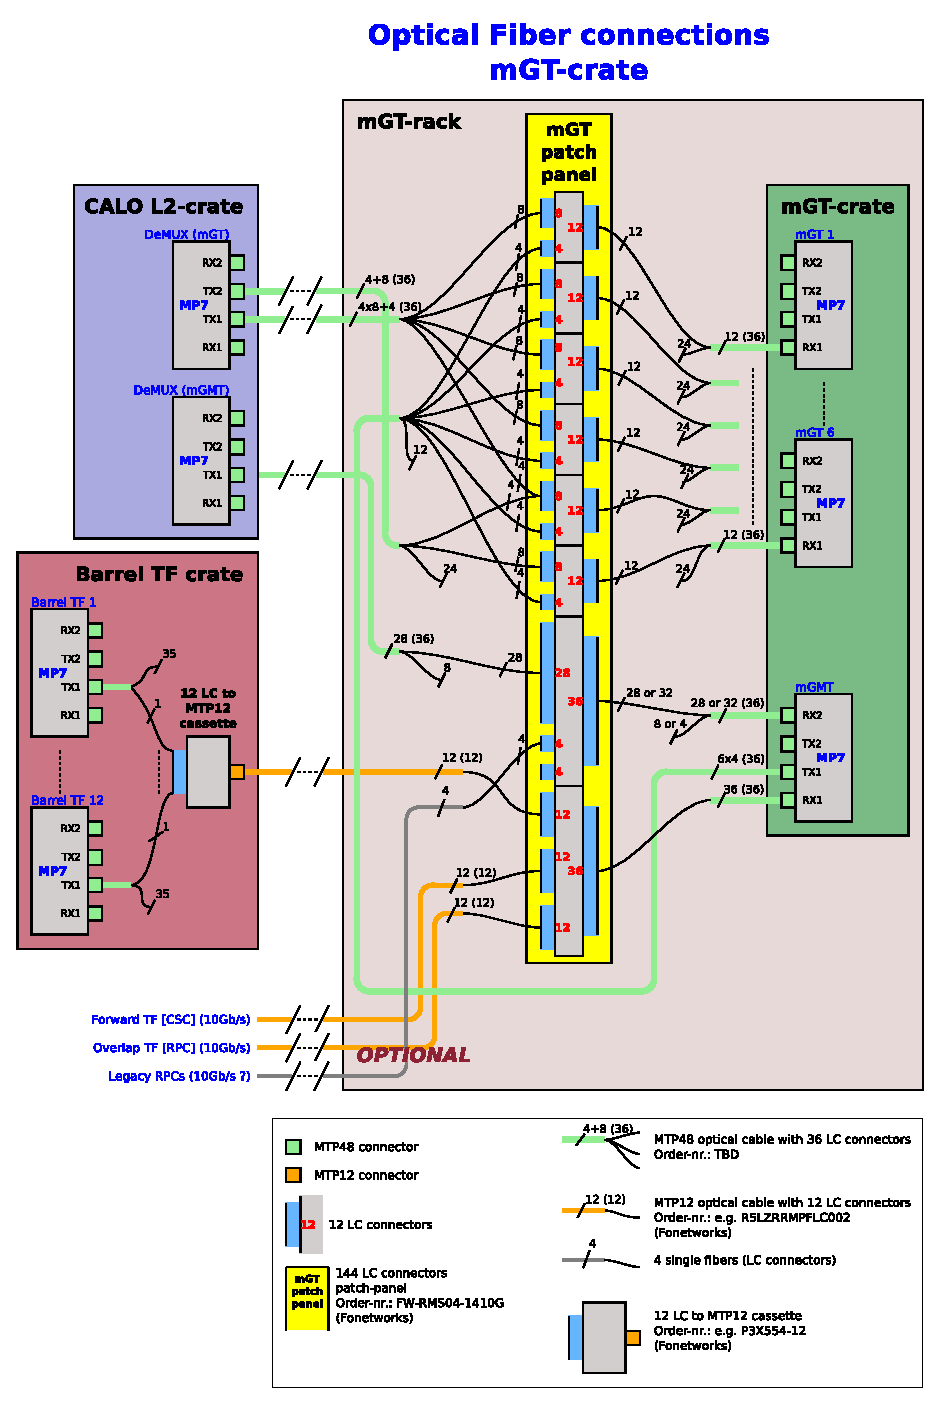
\includegraphics[width=14cm]{figures/mGT_mGMT_optical_connections}
\caption{Optical connections \ugt-crate} 
\label{fig:com-hard:mGT_mGMT_fiber_optical_patch}
\end{figure}

\clearpage

Figure \ref{fig:com-hard:mGT_mGMT_144_LC_patch_panel} shows the front panel of the patch panel - \textbf{first draft}.

\begin{figure}[htb]
\centering
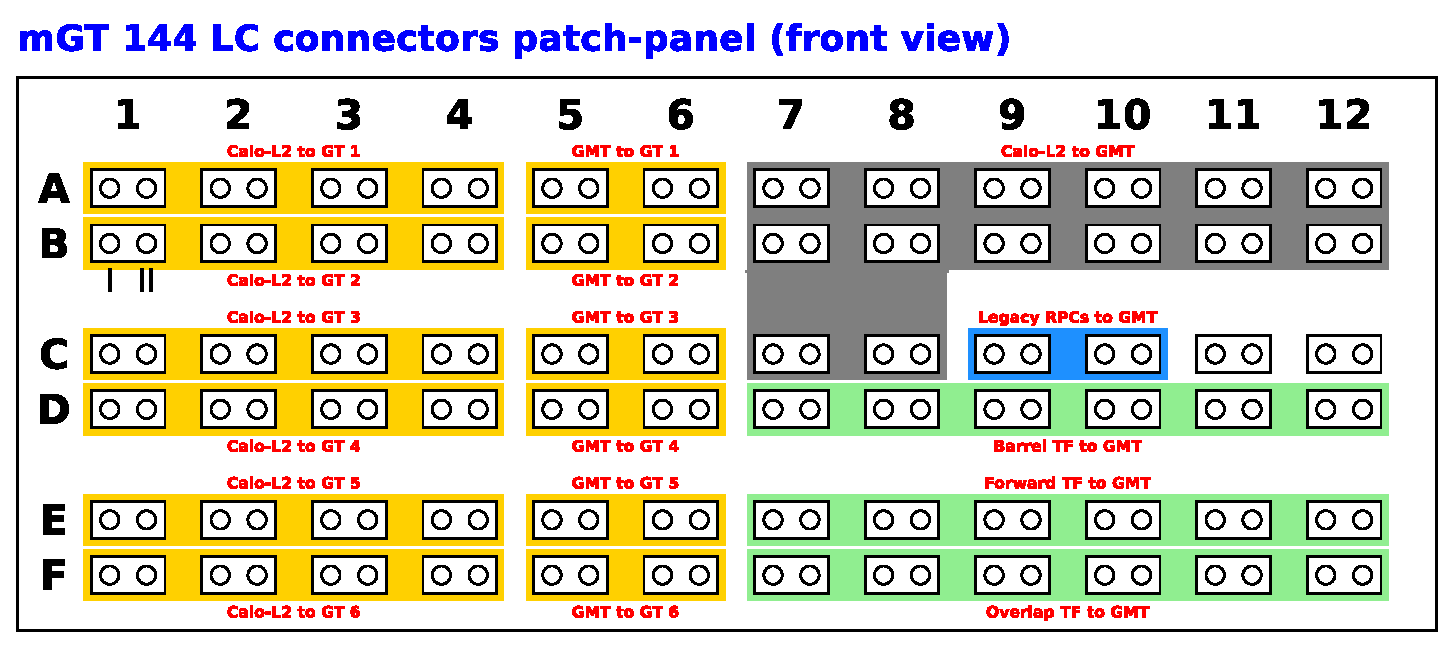
\includegraphics[width=14cm]{figures/mGT_mGMT_144_LC_patch_panel}
\caption{Optical patch-panel \ugt-crate (front view)} 
\label{fig:com-hard:mGT_mGMT_144_LC_patch_panel}
\end{figure}

\clearpage

Figures \ref{fig:com-hard:mGT_crate_optical_pp_connections} and \ref{fig:com-hard:mGT_crate_optical_pp_connections_2} 
show patching the LC connectors - \textbf{first draft}.

\begin{figure}[htb]
\centering
\includegraphics[width=14cm]{figures/mGT_crate_optical_pp_connections}
\caption{Optical connections on patch-panel \ugt-crate (part 1)} 
\label{fig:com-hard:mGT_crate_optical_pp_connections}
\end{figure}

\begin{figure}[htb]
\centering
\includegraphics[width=14cm]{figures/mGT_crate_optical_pp_connections_2}
\caption{Optical connections on patch-panel \ugt-crate (part 2)} 
\label{fig:com-hard:mGT_crate_optical_pp_connections_2}
\end{figure}

\clearpage

% Table \ref{tab:com-hard:mGT_mGMT_optical_connections_table} shows patching the LC connectors - \textbf{first draft}, has to be renewed because of Calo-L2 fiber connections.
% 
% \begin{longtable}{|p{.09\columnwidth}|p{.1\columnwidth}|p{.08\columnwidth}|p{.1\columnwidth}|p{.2\columnwidth}|p{.07\columnwidth}|p{.07\columnwidth}|p{.07\columnwidth}|}\hline 
% \textbf{Source mod. conn.} & \textbf{Source cable name} & \textbf{Source fiber} & \textbf{mGT patch-panel location} & \textbf{Data on fiber} & \textbf{Dest. fiber} & \textbf{Dest. cable name} & \textbf{Dest. mod. conn.}\\\hline\hline 
% \endhead
% \multirow{8}{16mm}{Calo-L2 DeMUX \ugt TX1} & \multirow{8}{15mm}{CALO 1} & 1  & A-1-I   & \egamma 0..5  & 1  & \multirow{12}{12mm}{GT 1} & \multirow{12}{12mm}{\ugt board 1 RX1}\\\cline{3-6}
%                                            &                            & 2  & A-1-II  & \egamma 6..11 & 2  &                           &                                      \\\cline{3-6}
%                                            &                            & 3  & A-2-I   & jet 0..5      & 3  &                           &                                      \\\cline{3-6}
%                                            &                            & 4  & A-2-II  & jet 6..11     & 4  &                           &                                      \\\cline{3-6}
%                                            &                            & 5  & A-3-I   & tau 0..5      & 5  &                           &                                      \\\cline{3-6}
%                                            &                            & 6  & A-3-II  & tau 6..11     & 6  &                           &                                      \\\cline{3-6}
%                                            &                            & 7  & A-4-I   & energy sums   & 7  &                           &                                      \\\cline{3-6}
%                                            &                            & 8  & A-4-II  & "not used"    & 8  &                           &                                      \\\cline{1-6}
% \multirow{4}{16mm}{\ugmt TX1}              & \multirow{4}{15mm}{GMT 3}  & 1  & A-5-I   & muon 0..1     & 9  &                           &                                      \\\cline{3-6}
%                                            &                            & 2  & A-5-II  & muon 2..3     & 10 &                           &                                      \\\cline{3-6}
%                                            &                            & 3  & A-6-I   & muon 4..5     & 11 &                           &                                      \\\cline{3-6}
%                                            &                            & 4  & A-6-II  & muon 6..7     & 12 &                           &                                      \\\hline
% \multirow{8}{16mm}{Calo-L2 DeMUX \ugt TX1} & \multirow{8}{15mm}{CALO 1} & 9  & B-1-I   & \egamma 0..5  & 1  & \multirow{12}{12mm}{GT 2} & \multirow{12}{12mm}{\ugt board 2 RX1}\\\cline{3-6}
%                                            &                            & 10 & B-1-II  & \egamma 6..11 & 2  &                           &                                      \\\cline{3-6}
%                                            &                            & 11 & B-2-I   & jet 0..5      & 3  &                           &                                      \\\cline{3-6}
%                                            &                            & 12 & B-2-II  & jet 6..11     & 4  &                           &                                      \\\cline{3-6}
%                                            &                            & 13 & B-3-I   & tau 0..5      & 5  &                           &                                      \\\cline{3-6}
%                                            &                            & 14 & B-3-II  & tau 6..11     & 6  &                           &                                      \\\cline{3-6}
%                                            &                            & 15 & B-4-I   & energy sums   & 7  &                           &                                      \\\cline{3-6}
%                                            &                            & 16 & B-4-II  & "not used"    & 8  &                           &                                      \\\cline{1-6}
% \multirow{4}{16mm}{\ugmt TX1}              & \multirow{4}{15mm}{GMT 3}  & 5  & B-5-I   & muon 0..1     & 9  &                           &                                      \\\cline{3-6}
%                                            &                            & 6  & B-5-II  & muon 2..3     & 10 &                           &                                      \\\cline{3-6}
%                                            &                            & 7  & B-6-I   & muon 4..5     & 11 &                           &                                      \\\cline{3-6}
%                                            &                            & 8  & B-6-II  & muon 6..7     & 12 &                           &                                      \\\hline
% \multirow{8}{16mm}{Calo-L2 DeMUX \ugt TX1} & \multirow{8}{15mm}{CALO 1} & 17 & C-1-I   & \egamma 0..5  & 1  & \multirow{12}{12mm}{GT 3} & \multirow{12}{12mm}{\ugt board 3 RX1}\\\cline{3-6}
%                                            &                            & 18 & C-1-II  & \egamma 6..11 & 2  &                           &                                      \\\cline{3-6}
%                                            &                            & 19 & C-2-I   & jet 0..5      & 3  &                           &                                      \\\cline{3-6}
%                                            &                            & 20 & C-2-II  & jet 6..11     & 4  &                           &                                      \\\cline{3-6}
%                                            &                            & 21 & C-3-I   & tau 0..5      & 5  &                           &                                      \\\cline{3-6}
%                                            &                            & 22 & C-3-II  & tau 6..11     & 6  &                           &                                      \\\cline{3-6}
%                                            &                            & 23 & C-4-I   & energy sums   & 7  &                           &                                      \\\cline{3-6}
%                                            &                            & 24 & C-4-II  & "not used"    & 8  &                           &                                      \\\cline{1-6}
% \multirow{4}{16mm}{\ugmt TX1}              & \multirow{4}{15mm}{GMT 3}  & 9  & C-5-I   & muon 0..1     & 9  &                           &                                      \\\cline{3-6}
%                                            &                            & 10 & C-5-II  & muon 2..3     & 10 &                           &                                      \\\cline{3-6}
%                                            &                            & 11 & C-6-I   & muon 4..5     & 11 &                           &                                      \\\cline{3-6}
%                                            &                            & 12 & C-6-II  & muon 6..7     & 12 &                           &                                      \\\hline
% \multirow{8}{16mm}{Calo-L2 DeMUX \ugt TX1} & \multirow{8}{15mm}{CALO 1} & 25 & D-1-I   & \egamma 0..5  & 1  & \multirow{12}{12mm}{GT 4} & \multirow{12}{12mm}{\ugt board 4 RX1}\\\cline{3-6}
%                                            &                            & 26 & D-1-II  & \egamma 6..11 & 2  &                           &                                      \\\cline{3-6}
%                                            &                            & 27 & D-2-I   & jet 0..5      & 3  &                           &                                      \\\cline{3-6}
%                                            &                            & 28 & D-2-II  & jet 6..11     & 4  &                           &                                      \\\cline{3-6}
%                                            &                            & 29 & D-3-I   & tau 0..5      & 5  &                           &                                      \\\cline{3-6}
%                                            &                            & 30 & D-3-II  & tau 6..11     & 6  &                           &                                      \\\cline{3-6}
%                                            &                            & 31 & D-4-I   & energy sums   & 7  &                           &                                      \\\cline{3-6}
%                                            &                            & 32 & D-4-II  & "not used"    & 8  &                           &                                      \\\cline{1-6}
% \multirow{4}{16mm}{\ugmt TX1}              & \multirow{4}{15mm}{GMT 3}  & 13 & D-5-I   & muon 0..1     & 9  &                           &                                      \\\cline{3-6}
%                                            &                            & 14 & D-5-II  & muon 2..3     & 10 &                           &                                      \\\cline{3-6}
%                                            &                            & 15 & D-6-I   & muon 4..5     & 11 &                           &                                      \\\cline{3-6}
%                                            &                            & 16 & D-6-II  & muon 6..7     & 12 &                           &                                      \\\hline
% \multirow{4}{16mm}{Calo-L2 DeMUX \ugt TX1} & \multirow{4}{15mm}{CALO 1} & 33 & E-1-I   & \egamma 0..5  & 1  & \multirow{12}{12mm}{GT 5} & \multirow{12}{12mm}{\ugt board 5 RX1}\\\cline{3-6}
%                                            &                            & 34 & E-1-II  & \egamma 6..11 & 2  &                           &                                      \\\cline{3-6}
%                                            &                            & 35 & E-2-I   & jet 0..5      & 3  &                           &                                      \\\cline{3-6}
%                                            &                            & 36 & E-2-II  & jet 6..11     & 4  &                           &                                      \\\cline{1-6}
% \multirow{4}{16mm}{Calo-L2 DeMUX \ugt TX2} & \multirow{4}{15mm}{CALO 2} & 1  & E-3-I   & tau 0..5      & 5  &                           &                                      \\\cline{3-6}
%                                            &                            & 2  & E-3-II  & tau 6..11     & 6  &                           &                                      \\\cline{3-6}
%                                            &                            & 3  & E-4-I   & energy sums   & 7  &                           &                                      \\\cline{3-6}
%                                            &                            & 4  & E-4-II  & "not used"    & 8  &                           &                                      \\\cline{1-6}
% \multirow{4}{16mm}{\ugmt TX1}              & \multirow{4}{15mm}{GMT 3}  & 17 & E-5-I   & muon 0..1     & 9  &                           &                                      \\\cline{3-6}
%                                            &                            & 18 & E-5-II  & muon 2..3     & 10 &                           &                                      \\\cline{3-6}
%                                            &                            & 19 & E-6-I   & muon 4..5     & 11 &                           &                                      \\\cline{3-6}
%                                            &                            & 20 & E-6-II  & muon 6..7     & 12 &                           &                                      \\\hline
% \multirow{8}{16mm}{Calo-L2 DeMUX \ugt TX2} & \multirow{8}{15mm}{CALO 2} & 5  & F-1-I   & \egamma 0..5  & 1  & \multirow{12}{12mm}{GT 6} & \multirow{12}{12mm}{\ugt board 6 RX1}\\\cline{3-6}
%                                            &                            & 6  & F-1-II  & \egamma 6..11 & 2  &                           &                                      \\\cline{3-6}
%                                            &                            & 7  & F-2-I   & jet 0..5      & 3  &                           &                                      \\\cline{3-6}
%                                            &                            & 8  & F-2-II  & jet 6..11     & 4  &                           &                                      \\\cline{3-6}
%                                            &                            & 9  & F-3-I   & tau 0..5      & 5  &                           &                                      \\\cline{3-6}
%                                            &                            & 10 & F-3-II  & tau 6..11     & 6  &                           &                                      \\\cline{3-6}
%                                            &                            & 11 & F-4-I   & energy sums   & 7  &                           &                                      \\\cline{3-6}
%                                            &                            & 12 & F-4-II  & "not used"    & 8  &                           &                                      \\\cline{1-6}
% \multirow{4}{16mm}{\ugmt TX1}              & \multirow{4}{15mm}{GMT 3}  & 21 & F-5-I   & muon 0..1     & 9  &                           &                                      \\\cline{3-6}
%                                            &                            & 22 & F-5-II  & muon 2..3     & 10 &                           &                                      \\\cline{3-6}
%                                            &                            & 23 & F-6-I   & muon 4..5     & 11 &                           &                                      \\\cline{3-6}
%                                            &                            & 24 & F-6-II  & muon 6..7     & 12 &                           &                                      \\\hline
% \multirow{28}{16mm}{Calo-L2 DeMUX \ugmt TX1} & \multirow{28}{15mm}{CALO 3} & 1  & A-7-I   & \multirow{28}{30mm}{???}       & 1  & \multirow{36}{15mm}{GMT 2} & \multirow{36}{12mm}{\ugmt RX2}     \\\cline{3-4}\cline{6-6}
%                                              &                             & 2  & A-7-II  &            & 2  &                           &                                    \\\cline{3-4}\cline{6-6}
%                                              &                             & 3  & A-8-I   &            & 3  &                           &                                    \\\cline{3-4}\cline{6-6}
%                                              &                             & 4  & A-8-II  &            & 4  &                           &                                    \\\cline{3-4}\cline{6-6}
%                                              &                             & 5  & A-9-I   &            & 5  &                           &                                    \\\cline{3-4}\cline{6-6}
%                                              &                             & 6  & A-9-II  &            & 6  &                           &                                    \\\cline{3-4}\cline{6-6}
%                                              &                             & 7  & A-10-I  &            & 7  &                           &                                    \\\cline{3-4}\cline{6-6}
%                                              &                             & 8  & A-10-II &            & 8  &                           &                                    \\\cline{3-4}\cline{6-6}
%                                              &                             & 9  & A-11-I  &            & 9  &                           &                                    \\\cline{3-4}\cline{6-6}
%                                              &                             & 10 & A-11-II &            & 10 &                           &                                    \\\cline{3-4}\cline{6-6}
%                                              &                             & 11 & A-12-I  &            & 11 &                           &                                    \\\cline{3-4}\cline{6-6}
%                                              &                             & 12 & A-12-II &            & 12 &                           &                                    \\\cline{3-4}\cline{6-6}
%                                              &                             & 13 & B-7-I   &            & 13 &                           &                                    \\\cline{3-4}\cline{6-6}
%                                              &                             & 14 & B-7-II  &            & 14 &                           &                                    \\\cline{3-4}\cline{6-6}
%                                              &                             & 15 & B-8-I   &            & 15 &                           &                                    \\\cline{3-4}\cline{6-6}
%                                              &                             & 16 & B-8-II  &            & 16 &                           &                                    \\\cline{3-4}\cline{6-6}
%                                              &                             & 17 & B-9-I   &            & 17 &                           &                                    \\\cline{3-4}\cline{6-6}
%                                              &                             & 18 & B-9-II  &            & 18 &                           &                                    \\\cline{3-4}\cline{6-6}
%                                              &                             & 19 & B-10-I  &            & 19 &                           &                                    \\\cline{3-4}\cline{6-6}
%                                              &                             & 20 & B-10-II &            & 20 &                           &                                    \\\cline{3-4}\cline{6-6}
%                                              &                             & 21 & B-11-I  &            & 21 &                           &                                    \\\cline{3-4}\cline{6-6}
%                                              &                             & 22 & B-11-II &            & 22 &                           &                                    \\\cline{3-4}\cline{6-6}
%                                              &                             & 23 & B-12-I  &            & 23 &                           &                                    \\\cline{3-4}\cline{6-6}
%                                              &                             & 24 & B-12-II &            & 24 &                           &                                    \\\cline{3-4}\cline{6-6}
%                                              &                             & 25 & C-7-I   &            & 25 &                           &                                    \\\cline{3-4}\cline{6-6}
%                                              &                             & 26 & C-7-II  &            & 26 &                           &                                    \\\cline{3-4}\cline{6-6}
%                                              &                             & 27 & C-8-I   &            & 27 &                           &                                    \\\cline{3-4}\cline{6-6}
%                                              &                             & 28 & C-8-II  &            & 28 &                           &                                    \\\cline{1-6}
% \multirow{4}{16mm}{Legacy RPC (optional)}    & \multirow{4}{15mm}{Legacy RPC (optional)} & 1  & C-9-I   & \multirow{4}{30mm}{legacy RPC (optional)} & 29 &    &              \\\cline{3-4}\cline{6-6}
%                                              &                                & 2  & C-9-II  &         & 30 &                           &                                    \\\cline{3-4}\cline{6-6}
%                                              &                                & 3  & C-10-I  &         & 31 &                           &                                    \\\cline{3-4}\cline{6-6}
%                                              &                                & 4  & C-10-II &         & 32 &                           &                                    \\\cline{1-6}
%                                              &                                &    & C-11-I  & "not used"   & 33 &                           &                                    \\\cline{1-6}
%                                              &                                &    & C-11-II & "not used"   & 34 &                           &                                    \\\cline{1-6}
%                                              &                                &    & C-12-I  & "not used"   & 35 &                           &                                    \\\cline{1-6}
%                                              &                                &    & C-12-II & "not used"   & 36 &                           &                                    \\\hline
% \multirow{12}{16mm}{Barrel TF (DT)} & \multirow{12}{15mm}{DT}     & 1  & D-7-I   & \multirow{12}{30mm}{Barrel TF} & 1  & \multirow{36}{15mm}{GMT 1} & \multirow{36}{12mm}{\ugmt RX1}\\\cline{3-4}\cline{6-6}
%                                     &                            & 2  & D-7-II  &                               & 2  &                            &                               \\\cline{3-4}\cline{6-6}
%                                     &                            & 3  & D-8-I   &                               & 3  &                            &                               \\\cline{3-4}\cline{6-6}
%                                     &                            & 4  & D-8-II  &                               & 4  &                            &                               \\\cline{3-4}\cline{6-6}
%                                     &                            & 5  & D-9-I   &                               & 5  &                            &                               \\\cline{3-4}\cline{6-6}
%                                     &                            & 6  & D-9-II  &                               & 6  &                            &                               \\\cline{3-4}\cline{6-6}
%                                     &                            & 7  & D-10-I  &                               & 7  &                            &                               \\\cline{3-4}\cline{6-6}
%                                     &                            & 8  & D-10-II &                               & 8  &                            &                               \\\cline{6-6}
%                                     &                            & 9  & D-11-I  &                               & 9  &                            &                               \\\cline{3-4}\cline{6-6}
%                                     &                            & 10 & D-11-II &                               & 10 &                            &                               \\\cline{3-4}\cline{6-6}
%                                     &                            & 11 & D-12-I  &                               & 11 &                            &                               \\\cline{3-4}\cline{6-6}
%                                     &                            & 12 & D-12-II &                               & 12 &                            &                               \\\cline{1-6}
% \multirow{12}{16mm}{Forward TF (CSC)} & \multirow{12}{15mm}{CSC}   & 1  & E-7-I   & \multirow{12}{30mm}{Forward TF}& 13 &                            &                               \\\cline{3-4}\cline{6-6}
%                                     &                            & 2  & E-7-II  &                               & 14 &                            &                               \\\cline{3-4}\cline{6-6}
%                                     &                            & 3  & E-8-I   &                               & 15 &                            &                               \\\cline{3-4}\cline{6-6}
%                                     &                            & 4  & E-8-II  &                               & 16 &                            &                               \\\cline{3-4}\cline{6-6}
%                                     &                            & 5  & E-9-I   &                               & 17 &                            &                               \\\cline{3-4}\cline{6-6}
%                                     &                            & 6  & E-9-II  &                               & 18 &                            &                               \\\cline{3-4}\cline{6-6}
%                                     &                            & 7  & E-10-I  &                               & 19 &                            &                               \\\cline{3-4}\cline{6-6}
%                                     &                            & 8  & E-10-II &                               & 20 &                            &                               \\\cline{6-6}
%                                     &                            & 9  & E-11-I  &                               & 21 &                            &                               \\\cline{3-4}\cline{6-6}
%                                     &                            & 10 & E-11-II &                               & 22 &                            &                               \\\cline{3-4}\cline{6-6}
%                                     &                            & 11 & E-12-I  &                               & 23 &                            &                               \\\cline{3-4}\cline{6-6}
%                                     &                            & 12 & E-12-II &                               & 24 &                            &                               \\\cline{1-6}
% \multirow{12}{16mm}{Overlap TF (RPC)} & \multirow{12}{15mm}{RPC}   & 1  & F-7-I   & \multirow{12}{30mm}{Overlap TF}& 25 &                            &                               \\\cline{3-4}\cline{6-6}
%                                     &                            & 2  & F-7-II  &                               & 26 &                            &                               \\\cline{3-4}\cline{6-6}
%                                     &                            & 3  & F-8-I   &                               & 27 &                            &                               \\\cline{3-4}\cline{6-6}
%                                     &                            & 4  & F-8-II  &                               & 28 &                            &                               \\\cline{3-4}\cline{6-6}
%                                     &                            & 5  & F-9-I   &                               & 29 &                            &                               \\\cline{3-4}\cline{6-6}
%                                     &                            & 6  & F-9-II  &                               & 30 &                            &                               \\\cline{3-4}\cline{6-6}
%                                     &                            & 7  & F-10-I  &                               & 31 &                            &                               \\\cline{3-4}\cline{6-6}
%                                     &                            & 8  & F-10-II &                               & 32 &                            &                               \\\cline{6-6}
%                                     &                            & 9  & F-11-I  &                               & 33 &                            &                               \\\cline{3-4}\cline{6-6}
%                                     &                            & 10 & F-11-II &                               & 34 &                            &                               \\\cline{3-4}\cline{6-6}
%                                     &                            & 11 & F-12-I  &                               & 35 &                            &                               \\\cline{3-4}\cline{6-6}
%                                     &                            & 12 & F-12-II &                               & 36 &                            &                               \\\hline
% \caption{Optical connections on patch-panel \ugt-crate}
% \label{tab:com-hard:mGT_mGMT_optical_connections_table}
% \end{longtable}

Table \ref{tab:com-hard:device_list_opt_items_gt_crate} shows component list, which we need to order and define with collaborators. 
\begin{table}[htdp]
\begin{center}
\begin{tabular}{|p{10mm}|p{16mm}|p{16mm}|p{13mm}|c|p{20mm}|p{20mm}|p{16mm}|}\hline
\textbf{crate} & \textbf{item} & \textbf{type} & \textbf{item name} & \textbf{qty.} & \textbf{order-nr.} & \textbf{distributor} & \textbf{provided by}\\\hline\hline
\ugt & optical patch-panel & 144xLC & mGT patch panel & 1 & FW-RMS04-1410G & Fonetworks & HEPHY Vienna\\\cline{2-7}
     & optical cable & MTP48-36xLC & GT1-GT6, GMT1-GMT3 & 9 & TBD (2m?) & Fonetworks (?) &  \\\cline{2-7}
     & connector cleaners & smart cleaner &  & 2 & SMART-LC & Fonetworks &  \\\cline{3-7}
     & & reel cleaner &  & 2 & CRC02 & Fonetworks &  \\\cline{3-7}
     & & in adapter cleaner &  & 2 & MTP-IBC & Fonetworks &  \\\hline
Calo-L2 & optical cable & MTP48-36xLC & CALO1-CALO3 & 3 & TBD (5m?) & Fonetworks & Imperial College (?)\\\hline
DT   & optical cassette & 12xLC-MTP12 & DT cassette & 1 & e.g. P3X554-12 & Fonetworks & HEPHY Vienna\\\cline{2-7}
     & optical cable & MTP12-12xLC & DTOUT & 1 & similar: R5LZRR-MPLFC002 (10m?) & Fonetworks &  \\\cline{2-7}
     & optical cable & MTP48-36xLC & DT1-DT12 & 12 & TBD (1m?) & Fonetworks &  \\\hline
CSC  & optical cable & e.g. MTP12-12xLC or 12xLC single fibers & CSC & 1 & TBD & Fonetworks & ???\\\hline
RPC  & optical cable & e.g. MTP12-12xLC or 12xLC single fibers & RPC & 1 & TBD & Fonetworks & ???\\\hline
\end{tabular}
\end{center}
\caption{Device list optical items \ugt-crate}
\label{tab:com-hard:device_list_opt_items_gt_crate}
\end{table}

\clearpage

\subsection{External conditions connections for \ugt-crate}\label{sec:com-hard:external_cond}

The \ugt-system receives external conditions as LVDS-signals on cables with RJ45-connectors. Therefore we need a conversion from parallel
to serial for receiving external conditions in \ugt firmware on MP7 modules.\\
The conversion is done in two stages:
\begin{itemize}
\item First stage: collecting each 32 external conditions to groups and changing the connector type to VHDCI.
\item Second stage: converting parallel data structure to serial data on GLIB3 (or FC7) modules and sending it via backplane to MP7 modules in \ugt-crate.
\end{itemize}
The first stage is done with a "RJ45-VHDCI patch-panel" (see Figure \ref{fig:com-hard:mGT_rj45_vhdci_patch_panel}),
where external conditions signals on RJ45 connectors are grouped to VHDCI connectors. A "RJ45-VHDCI patch-panel" contains 4 units of "RJ45-VHDCI converter"
(see also Figures \ref{fig:com-hard:rj45_vhdci_patchpanel_1}, \ref{fig:com-hard:rj45_vhdci_patchpanel_2} and \ref{fig:com-hard:rj45_vhdci_patchpanel_5}).
From there, VHDCI cables (Molex, 799180080, 1m - \textbf{length not decided yet}) make the connection to FMC modules (HFMC LVDS Receiver) on GLIB3 (or FC7) modules
(see Figures \ref{fig:com-hard:hfmc_lvds_mezzanine} and \ref{fig:com-hard:hfmc_lvds_mezz_glib}).
Every of 4 GLIB3 (or FC7) module can convert 64 external conditions signals to serial data (5Gb/s), which are sent over the backplane on AMC ports 4-7 and a CBS (on MCH)
to the \ugt-modules (MP7).\\
The "RJ45-VHDCI patch-panel" will be located on the rear side of \ugt-rack (USC55), to prevend a lot of RJ45-cables on the front of the rack (see also Figures
\ref{fig:com-hard:mGT_rack_cabling} and \ref{fig:com-hard:mGT_rack_cabling_views}).

\begin{figure}[htb]
\centering
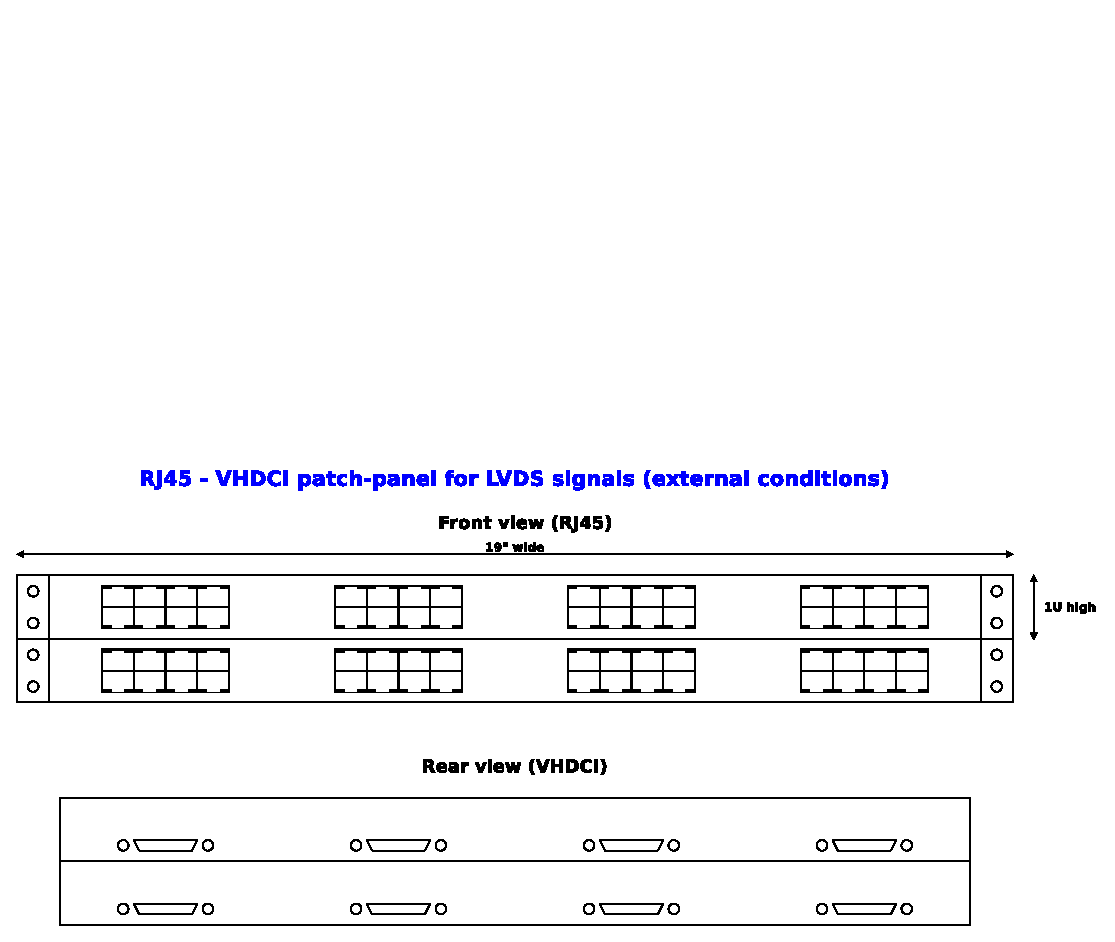
\includegraphics[width=14cm]{figures/mGT_rj45_vhdci_patch_panel}
\caption{RJ45 -VHDCI patch-panel for external conditions in \ugt-crate} 
\label{fig:com-hard:mGT_rj45_vhdci_patch_panel}
\end{figure}

\begin{figure}[htb]
\centering
\includegraphics[width=14cm]{figures/RJ45_VHDCI_Patchpanel_1}
\caption{"RJ45-VHDCI converter" back side (VHDCI)} 
\label{fig:com-hard:rj45_vhdci_patchpanel_1}
\end{figure}

\begin{figure}[htb]
\centering
\includegraphics[width=14cm]{figures/RJ45_VHDCI_Patchpanel_2}
\caption{"RJ45-VHDCI converter" front side (RJ45)} 
\label{fig:com-hard:rj45_vhdci_patchpanel_2}
\end{figure}

\begin{figure}[htb]
\centering
\includegraphics[width=14cm]{figures/RJ45_VHDCI_Patchpanel_5}
\caption{"RJ45-VHDCI converter" with cables} 
\label{fig:com-hard:rj45_vhdci_patchpanel_5}
\end{figure}

\begin{figure}[htb]
\centering
\includegraphics[width=14cm]{figures/HFMC_LVDS_mezzanine}
\caption{HFMC LVDS mezzanine} 
\label{fig:com-hard:hfmc_lvds_mezzanine}
\end{figure}

\begin{figure}[htb]
\centering
\includegraphics[width=14cm]{figures/HFMC_LVDS_mezz_GLIB}
\caption{HFMC LVDS mezzanine on GLIB2} 
\label{fig:com-hard:hfmc_lvds_mezz_glib}
\end{figure}

\clearpage

\subsection{Arrangement of \ugt-crate and patch-panels in \ugt-rack}\label{sec:com-hard:cabling_mgt_rack}

The arrangement and the cabling between \ugt-crate and patch-panels is \textbf{very preliminary}. For exact arrangement all the dimension are to known.\\
In Figure \ref{fig:com-hard:mGT_rack_cabling} one can see, how the cabling between the patch-panels and the \ugt-crate could be done. On the back side of the \ugt-rack
all the "external" cables are connected to the patch-panels, 64 RJ45-cables for the external condition data (max. 256 bits), 2 MTP48 optical cables with 36 LC connectors
for Calo-L2 data to \ugt, 1 MTP48 optical cable with 36 LC connectors for Calo-L2 data to \ugmt and 3 MTP12 optical cables with 12 LC connectors for data from Barrel TF,
Forward TF and Overlap TF. In addition there is a "internal" cable from \ugmt to optical patch-panel for \ugmt output data to \ugt (1 MTP48 optical cable with 36 LC connectors).\\
The connections from the patch-panels to \ugt-crate are made with 8 VHDCI 68 cables to HFMC (mezzanine board) on GLIB3 and with 8 MTP48 optical cables with 36 LC connectors
to MP7 modules (6 for \ugt, 2 for \ugmt). See also Section \ref{sec:com-hard:external_cond} and Figure \ref{fig:com-hard:mGT_mGMT_fiber_optical_patch}.\\
In Figure \ref{fig:com-hard:mGT_rack_cabling_views} a scheme of the arrangement of \ugt-crate and patch-panels within the \ugt-rack is shown in three views (top, front and back).\\
\textbf{Remark}: if there is not enough space for a height of 10U (7U \ugt-crate, 2U "RJ45-VHDCI patch-panel" and 1U "\finor patch-panel"),
the "RJ45-VHDCI patch-panel" could be arranged behind the \ugt-crate at the same height of top as the top of the \ugt-crate, which would need only 8U.

\begin{figure}[htb]
\centering
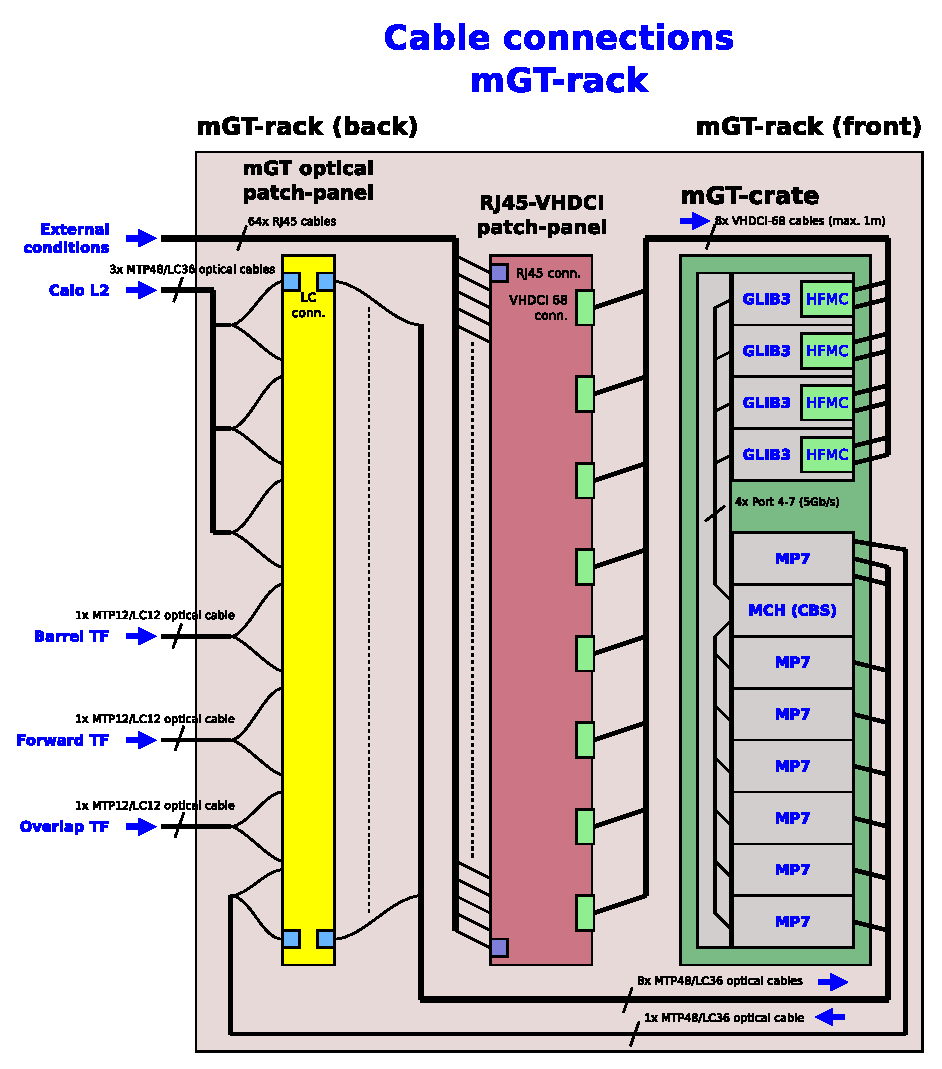
\includegraphics[width=14cm]{figures/mGT_rack_cabling}
\caption{Cable connections in \ugt-rack (top view)} 
\label{fig:com-hard:mGT_rack_cabling}
\end{figure}

\clearpage

\begin{figure}[htb]
\centering
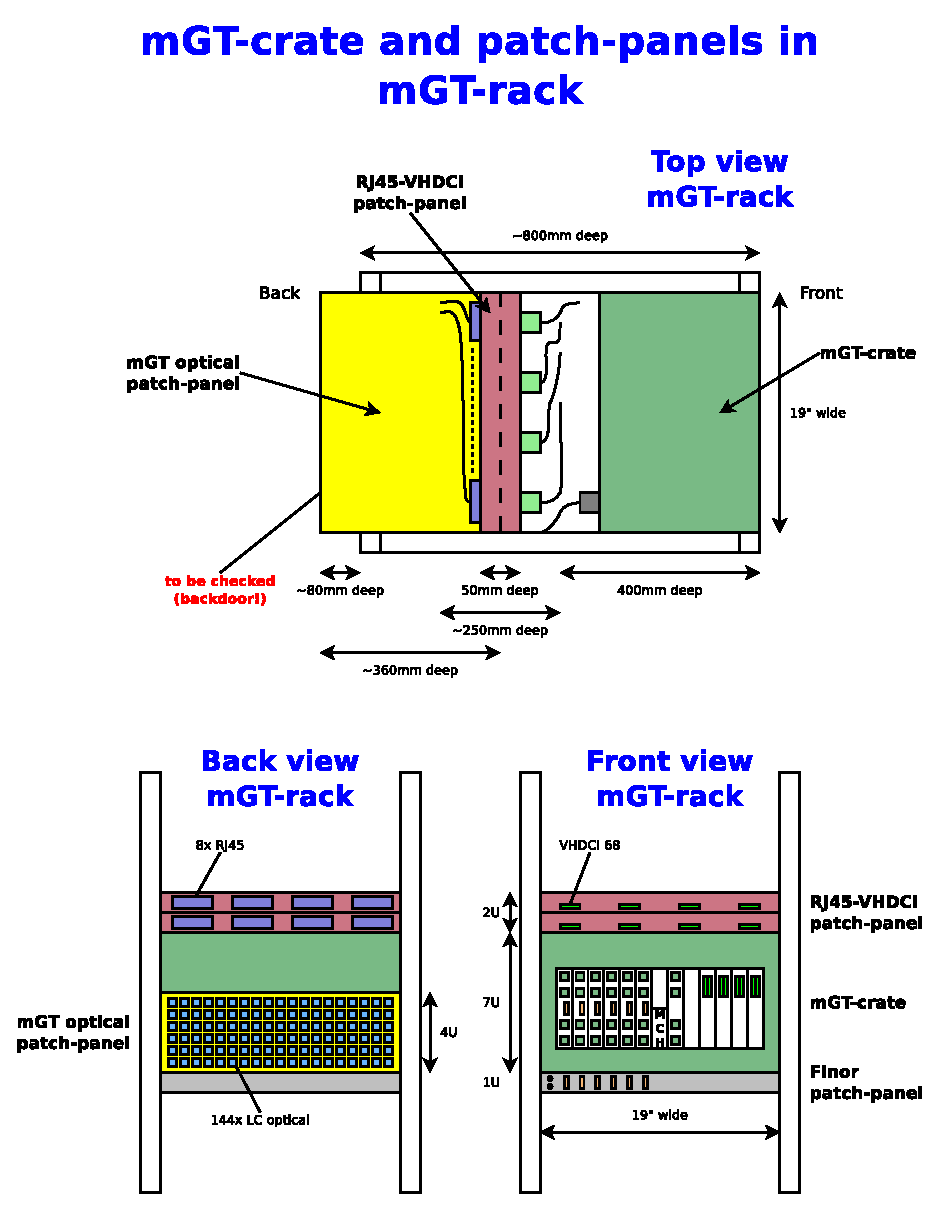
\includegraphics[width=14cm]{figures/mGT_rack_cabling_views}
\caption{Views of \ugt-crate and patch-panels in \ugt-rack} 
\label{fig:com-hard:mGT_rack_cabling_views}
\end{figure}

% % ------------------------------------------------------------------------------
%
% Repository path   : $HeadURL: https://hbergauer@forge.hephy.oeaw.ac.at/scm/svn/project-cmstrigger/GlobalTriggerUpgrade/doc/latex/gt-mp7-firmware-specification/content/requirements.tex $
% Last committed    : $Revision: 4401 $
% Last changed by   : $Author: hbergauer $
% Last changed date : $Date: 2016-11-03 14:48:50 +0100 (Thu, 03 Nov 2016) $
% Description       : Requirements
% ------------------------------------------------------------------------------
\section{Requirements}\label{sec:req}
\textbf{\textit{Under construction!!!}}

% The following requirements are defined and released until end of LS1.
% 
% 
% % ------------------------------------------------------------------------------
% %
% %  Design Guide Rules
% %
% % ------------------------------------------------------------------------------
% \subsection{Design Guide Rules}
% \textbf{R\_DGR\_1:} Same code for simulation as well as synthesis process.\\
% \textbf{R\_DGR\_2:} Use records where beneficial.\\
% \textbf{R\_DGR\_3:} All constants have to be defined in: \verb|gt_mp7_pkg.vhd|, \verb|rop_mp7_pkg.vhd|, \verb|gtl_mp7_pkg.vhd|, \verb|fdl_mp7_pkg.vhd|.\\
% \textbf{R\_DGR\_4:} All components of the design should be defined in: \verb|gt_amc514_lib.vhd|.\\
% \textbf{R\_DGR\_5:} All VHDL modules should be simulated as well as synthesized and tested at hardware.\\
% \textbf{R\_DGR\_6:} The specification should be found in GlobalTriggerUpgrade repository.\\
% \textbf{R\_DGR\_7:} The long term test as well as short term test should be specified together with software team. There are some scripts (e.g. pyhton, shell,etc) to start the test systematic for whole
% design as well as for each module.\\
% \textbf{R\_DGR\_8:} Python scripts, which allows to access and configure all modules in the firmware. It consists a general usage message that lists all subcommands
% and the common optional and required arguments can be obtained by <gtmp7-control.py> -h\\
% 
% % ------------------------------------------------------------------------------
% %
% %  Module Interfacing
% %
% % ------------------------------------------------------------------------------
% \subsection{Module Interfacing}\label{sec:minter}
% \textbf{R\_MIF\_1:} \verb|ORBIT| signal will be received through AMC13 over Bgos. This signal is 25 ns with periode of 89.1 us. We will synhronize this signal, in oder to be sure that we have 25 ns signal. We will check it, if we get 0xdeb (3563),it 
% means it is synchorn.\\
% \textbf{R\_MIF\_2:} \verb|L1A| signal will be received over AMC13.\\
% \textbf{R\_MIF\_3:} \verb|LHC clock| signal will be received over AMC13\\
% \textbf{R\_MIF\_4:} \verb|Readout-record| will be sent to AMC13. The size of it is limited to 4 KBytes per slot. \\
% \textbf{R\_MIF\_5:} \verb|TTC_decoder.vhd| deliver 2 data word named A and B over prot 3 (TTC). The word A is \verb|L1A| and word B is serial encoded data \verb|Bgos|\\
% 
% %------------------------------------------------------------------------------
% %
% %  SERDES
% %
% % ------------------------------------------------------------------------------
% \subsection{\serdes} \label{sec:serdes}
% is under construction...
% 
% \textbf{R\_SERDES\_1:} under construction \\
% \textbf{R\_SERDES\_2:} under construction \\
% ----------------------------------------------
% %
% %  IPBus
% %
% % ------------------------------------------------------------------------------
% \subsection{IPbus}\label{sec:req-ad}
% \textbf{R\_IBUS\_1:} under construction \\
% \textbf{R\_IBUS\_2:} under construction \\
% 
% 
% %------------------------------------------------------------------------------
% %
% %  Delay Manager
% %
% % ------------------------------------------------------------------------------
% \subsection{Delay Manager (\ac{DM})} \label{sec:req-dm}
% 
% \textbf{R\_DM\_1:} Every object type must have an individual delay. \\
% \textbf{R\_DM\_2:} The delay manager must produce two delayed versions of the bcres signal(for TCM and FDL). \\
% \textbf{R\_DM\_3:} The delay (given in lhc\_clk cycles) can be changed by software registers. \\
% \textbf{R\_DM\_4:} After the valid\_i signal is asserted, a valid lhc\_data is presented on the output after the longest individual delay. \\
% \textbf{R\_DM\_5:} Valid output data is indicated by asserting valid\_o. \\
% \textbf{R\_DM\_6:} If valid\_i is deasserted during operation valid\_o is also immediately deasserted. \\
% \textbf{R\_DM\_7:} The maximum time an individual object can be delay, must be configurable by a genereic.\\
% 
% 
% %------------------------------------------------------------------------------
% %
% %  SIM/SPY
% %
% % ------------------------------------------------------------------------------
% \subsection{SIM/SPY Memories} \label{sec:req-sim_spy}
% 
% \textbf{R\_MEM\_1:} Access to SIM memory, SPY memory I and SPY memory II. \\
% \textbf{R\_MEM\_1.1:} The SPY memory should be able to record one orbit data (3564). \\
% \textbf{R\_MEM\_1.2:} The SPY memory should be readable through software register access. \\ 
% \textbf{R\_MEM\_1.3:} The SIM memory should be writeable through software register access. \\
% \textbf{R\_MEM\_1.4:} The SIM memory should provide (simulated) orbit data to the DSMUX \\
% %\textbf{R\_MEM\_1.5:} The SIM memory and the SPY memory I should support multiple (parameterizable) channels. \\
% 
% %\textbf{R\_MEM\_2:} The port sizes should be customizable to the size of a single entry (16, 32 or 64). \\
% %\textbf{R\_MEM\_2.1:} The size of memories and the number of the memories should be correlated to object size and object number. The number of objects represents the number of memories and the resolution of each objects represents data-width. \\
% 
% \textbf{R\_MEM\_2:} The SPY memory should record the next whole orbit data after receiving the SPY NEXT trigger. \\
% \textbf{R\_MEM\_3:} The SPY memory should record a whole software selectable orbit data after receiving the SPY ONCE trigger. \\
% \textbf{R\_MEM\_4:} It should be possible to trigger SPY ONCE/NEXT by software register access.  \\
% \textbf{R\_MEM\_4.1:} The orbit number associated with the SPY ONCE trigger must also be software selectable. \\ 
% \textbf{R\_MEM\_4.2:} The status of the SPY memory and trigger must be indicated to the software in form of busy, ready and error flags.  \\
% \textbf{R\_MEM\_5:} The SPY trigger shall be issuable to multiple SPY memories (e.g., SPY memory I (all channels), SPY memory II) at once.
% Then the same orbit should be considered for all of them. \\
% 
% \textbf{R\_MEM\_6:} To capture ROP data, a special SPY memory (SPY~memory~III) should be implemented, which records blocks (split in 64-bit entries). \\
% \textbf{R\_MEM\_6.1:} The maximum size is 4kB (2048 16-bit words). Data is sent over Fabric A in 8b/10bG encoded packets of maximum length 4kB (2048 16-bit words). \\
% \textbf{R\_MEM\_6.1:} The input of SPY memory III should be parametrized for 16-bit, 32-bit, 64-bit, in order to adapt with TX (AMC13). \\
% \textbf{R\_MEM\_6.2:} The memory should record a single entry in case it's write enable signal is driven high. \\
% \textbf{R\_MEM\_6.3:} The memory should be readable through software register access. \\
% \textbf{R\_MEM\_6.4:} The memory should be able to record data from the DAQ clock domain. \\
% 
% %------------------------------------------------------------------------------
% %
% %  TCM
% %
% % ------------------------------------------------------------------------------
% 
% \subsection{Timing Counter Manager (TCM)} \label{sec:req-tcm}
% 
% \begin{itemize}
% \item [\req{TCM}{1}] The \ac{TCM} must provide counters for bunch crossings (\verb|bx_nr|, 12 bits),
% orbits (\verb|orbit_nr|, 48 bits), events (\verb|event_nr|, 32 bits) and luminosity segments (\verb|luminosity_seg_nr|, 32 bits) and tringger Nr (\verb|trigger_nr|, 48 bits).
% 
% \begin{itemize}
% \item [\req{TCM}{1.1}] All counters will be set to 0 after the ROSE process.
% \begin{itemize}
%  \item \textbf{R} (Resync-0x1): \verb|event_nr| will be set to 0
%  \item \textbf{O} (Oribit counter reset-0x8): \verb|orbit_nr| and \verb|luminosity_seg_nr| and tringger Nr (\verb|trigger_nr| will be set to 0
%  \item \textbf{S} (Start Run-0x9):\verb|trigger_nr| will be set to 0
%  \item \textbf{E} (Even counter reset): \verb|event_nr| will be set to 0
% \end{itemize}
% 
% \item [\req{TCM}{1.2}] The bunch crossing counter \verb|bx_nr| will be increased by 1 with \verb|lhc_clk|, and it counts the orbit signal, which is maybe 25 ns with the periode of 89.1 us. Therefore the counters coutes from 0-3563 (0xdeb) 
% It will be reset by \verb|BC0|, which we get over Bgos (0x1). 
% \item [\req{TCM}{1.3}] The event counter \verb|event_nr| counts the number of L1A, it means it will be increased after each L1A.
% \item [\req{TCM}{1.4}] The overflow of \verb|bx_nr| occures the increasing of the \verb|orbit_nr| by one.
% \item [\req{TCM}{1.5}] The luminosity segment Nr \verb|luminosity_seg_nr| will be increase by 1, if \verb|orbit_nr(18)| asserts to one. It will be happen over a 32-bit count compare condition
% (configurable through sofware register access). In case of bit(18)(lumisection = 23 sec = $2^{18} orbits)$, the compare condition of \verb|orbit_nr| is every 0x40000 (262144), which increases the \verb|luminosity_seg_nr| by one.
% \item [\req{TCM}{1.6}] FDL should receive a signal called \verb|start_lumisection| which is a 25ns pulse. Each time \verb|luminosity_seg_nr| is increased by one, a 25 ns signal will be produced. It means a signal with 25 ns of 23 sec period. \\
% 
% \end{itemize}
% 
% \item [\req{TCM}{2}] The assertion of \verb|bcres(BC0)| could always coincide with
% the counter \verb|bcres_nr| that it reaches the maximum number of bunch crossings (\verb|bcres_nr=3564(=0)|) or coincede with a
% defined counter \verb|bcres_nr| reset request (see requirements \req{TCM}{3.1} and \req{TCM}{3.5}).
% Moreover the \ac{TCM} enters a hardware error state and finsh any counting operation until the hardware error state is cleared (see \req{TCM}{3.2}).
% 
% \item [\req{TCM}{3}] TCM should handle BGos, which it gets from \utcs
% 
% 
% \begin{itemize}
% \item [\req{TCM}{3.1}] The command BC0 (''0001'') could coincide with the signal \verb|orbit| and should reset the counter \verb|bcres_nr| without triggering a hardware error state.
% \item [\req{TCM}{3.2}] The command HardReset (''0110'') should clear the error state.
% \item [\req{TCM}{3.3}] The command EC0 (''0111'') should reset the counter \verb|event_nr|.
% \item [\req{TCM}{3.4}] The command OC0 (''1000'') should reset the counter \verb|orbit_nr|
% \item [\req{TCM}{3.5}] The command RESYNC (''0101'') should reset the counter (see requirements \req{TCM}{1.1}).
% \item [\req{TCM}{3.6}] The command NOP (''0000'') should indicate that no special operation needs to be carried out.
% \item [\req{TCM}{3.7}] All BGOs commands are issued exactly one cycle with the exception of NOP.
% \end{itemize}
% %\item [\req{TCM}{4}] The \ac{TCM} must be implemented in its own VHDL module.
% \end{itemize}
% 
% 
% %-------------------------------------------------------------------------------
% %  GTL
% %
% % ------------------------------------------------------------------------------
% 
% \subsection{\gtl (\ugtl)} \label{sec:gtl}
% 
% \begin{itemize}
% \item [\req{GTL}{1}] \ugtl should receive data from \gct: 12 Electron/photon objects, 12 Jet objects, 8 Tau objects and 4 quantities of Energy summary information.
% All with a 32-bit data structure.\\
% \ugtl should receive data from \gmt: 8 objects with a 64-bit data structure. \\\ugtl should receive at least 256 External Conditions.
% \item [\req{GTL}{2}] \ugtl should provide following conditions:
% \begin{itemize}
% \item Calorimeter objects conditions
% \item Muon objects conditions
% \item Energy Summary Information conditions
% \item Correlation conditions
% \item Invariant-Mass conditions and Delta-R conditions
% \end{itemize}
% \item [\req{GTL}{3}] All these conditions should be made with data from bunch crossings (bx) within a +/-2 bx-range, if required.
% \item [\req{GTL}{4}] \ugtl should provide at least 512 Algorithms as output to \ufdl.
% \end{itemize}
% 
% %------------------------------------------------------------------------------
% %
% %  FDL
% %
% % ------------------------------------------------------------------------------
% \subsection{\fdl (\ufdl)} \label{sec:fdl}
% 
% \begin{itemize}
% \item [\req{FDL}{1}] \ufdl should receive at least 512 Algorithms from \ugtl. \\\ufdl should send one \finor to \utcs. 
% \item [\req{FDL}{2}] \ufdl should provide prescalers and rate-counters per Algorithm.
% \item [\req{FDL}{3}] \ufdl should provide algo-bx-mask, \finor-mask and veto-mask per Algorithm.
% \item [\req{FDL}{4}] \ufdl should provide Algorithms before prescalers, after prescalers, after masks and the local \finor and a total \finor for \record.
% \item [\req{FDL}{5}] \ufdl should provide a logic for updating the values of prescale-factors, reading and reseting the rate-counters.
% \item [\req{FDL}{6}] \ufdl should receive a signal called "begin\_lumi\_section" which is a 25ns pulse. With this signal updating the values of prescale-factors into prescalers, 
% storing the values of rate-counters in registers for reading and reseting the rate-counters is done.
% \item [\req{FDL}{7}] \ufdl should provide an interface to get software access to registers, counters and memories.
% \item [\req{FDL}{8}] \ufdl should provide two \finor: a local \finor and a total \finor. Both are inputs of ROP. The local \finor is send to \ugt board, which is the "total \finor board",
% if more than one \ugt boards are used.\\
% \end{itemize}
% %------------------------------------------------------------------------------
% %
% %  ROP
% %
% % ------------------------------------------------------------------------------
% \subsection{\rop (\ac{ROP})} \label{sec:rop}
% 
% \begin{itemize}
% \item [\req{ROP}{1}] 
% \item [\req{ROP}{2}] 
% \item [\req{ROP}{3}]
% \item [\req{ROP}{4}] 
% \end{itemize}
% 
% \clearpage

\clearpage


%------------------------------------------------------------------------------
%
% Repository path   : $HeadURL: https://hbergauer@forge.hephy.oeaw.ac.at/scm/svn/project-cmstrigger/GlobalTriggerUpgrade/doc/latex/gt-mp7-firmware-specification/content/firmware.tex $
% Last committed    : $Revision: 4401 $
% Last changed by   : $Author: hbergauer $
% Last changed date : $Date: 2016-11-03 14:48:50 +0100 (Thu, 03 Nov 2016) $
% Description       : firmware
% ------------------------------------------------------------------------------
\section{Firmware overview}\label{sec:fw}

The figure \ref{fig:mgt} shows the architecture of \ugt payload. It consists of framework, IPBus, output mux and the ALGORITHM LOGIC, which it consists of the following modules:
\begin{enumerate}
\item \ugtl
\item \ufdl
\end{enumerate}

The output mux collects data for read-out record which are send via MP7 read-out to AMC13.
 
The IPBus system allows the control of hardware via a ‘virtual bus’, using a standard IP-over-gigabit-Ethernet network connection (section [\ref{sec:ipbus}]).
\begin{figure}[h!]
   \centering
    \includegraphics[width=1.0\textwidth]{figures/mGT_payload}
    \caption{\ugt payload}\label{fig:mgt}
 \end{figure}
 
Moreover the \verb|Tx_AMC13| should be instanitate for sending the readout-record to AMC13. This part is outside of framework functionality.

\clearpage

%------------------------------------------------------------------------------
%
%  LHC data Packagee
%
% ------------------------------------------------------------------------------

\subsection{Package: lhc\_data\_pkg} \label{section_lhc_data_pkg}
% \textbf{\textit{Under construction!!!}}

The VHDL record \texttt{lhc\_data\_t} (shown in Listing \ref{lst_lhc_data_t}) is used as a container for all object streams processed by the system. It is declared in the VHDL package \texttt{lhc\_data\_pkg}.
% This package is auto-generated by the python script \texttt{lhc\_data\_pkg\_generator} from the XML specification in Listing \ref{lst_lhc_data_t_xml}. The script generates the record type, converter functions (to/from \texttt{std\_logic\_vector}) and various constants used by other modules in the system. 
For debugging and simulation purposes a second package (\texttt{lhc\_data\_debug\_util\_pkg}) is created which contains functions to convert the \texttt{lhc\_data\_t} to a hexadecimal string representation and vice versa. The testbench of the design uses this functions to load the contents of the SIM memory from a file. 

\lstinputlisting[label=lst_lhc_data_t,language=VHDL,caption=lhc\_data\_t record specification]{interfaces/lhc_data_t.vhd}

% \lstinputlisting[label=lst_lhc_data_t_xml,language=XML,caption=lhc\_data\_t xml specification]{../../../firmware/gt_amc514/trunk/xml/lhc_data_t.xml}
% 

\clearpage

%------------------------------------------------------------------------------
%
% Repository path   : $HeadURL: https://hbergauer@forge.hephy.oeaw.ac.at/scm/svn/project-cmstrigger/GlobalTriggerUpgrade/doc/latex/gt-mp7-firmware-specification/content/framework.tex $
% Last committed    : $Revision: 4485 $
% Last changed by   : $Author: hbergauer $
% Last changed date : $Date: 2018-08-13 16:51:08 +0200 (Mon, 13 Aug 2018) $
% Description       : framework
% ------------------------------------------------------------------------------
\section{Framework}\label{sec:framework}
\textbf{Remark:}\\
with frame v1.2.3 "Delay Manager" (dm.vhd) and "Data Source Multiplexer" (dsmux.vhd) are removed because these features were never used in production system, only for tests.
Simmem data not useable anymore, because of removed dsmux.
The reason of removing is to get more available resources.\\

Figure \ref{fig_system_overview} shows the basic components the framework together with \rop. 
 
\begin{figure}[h]
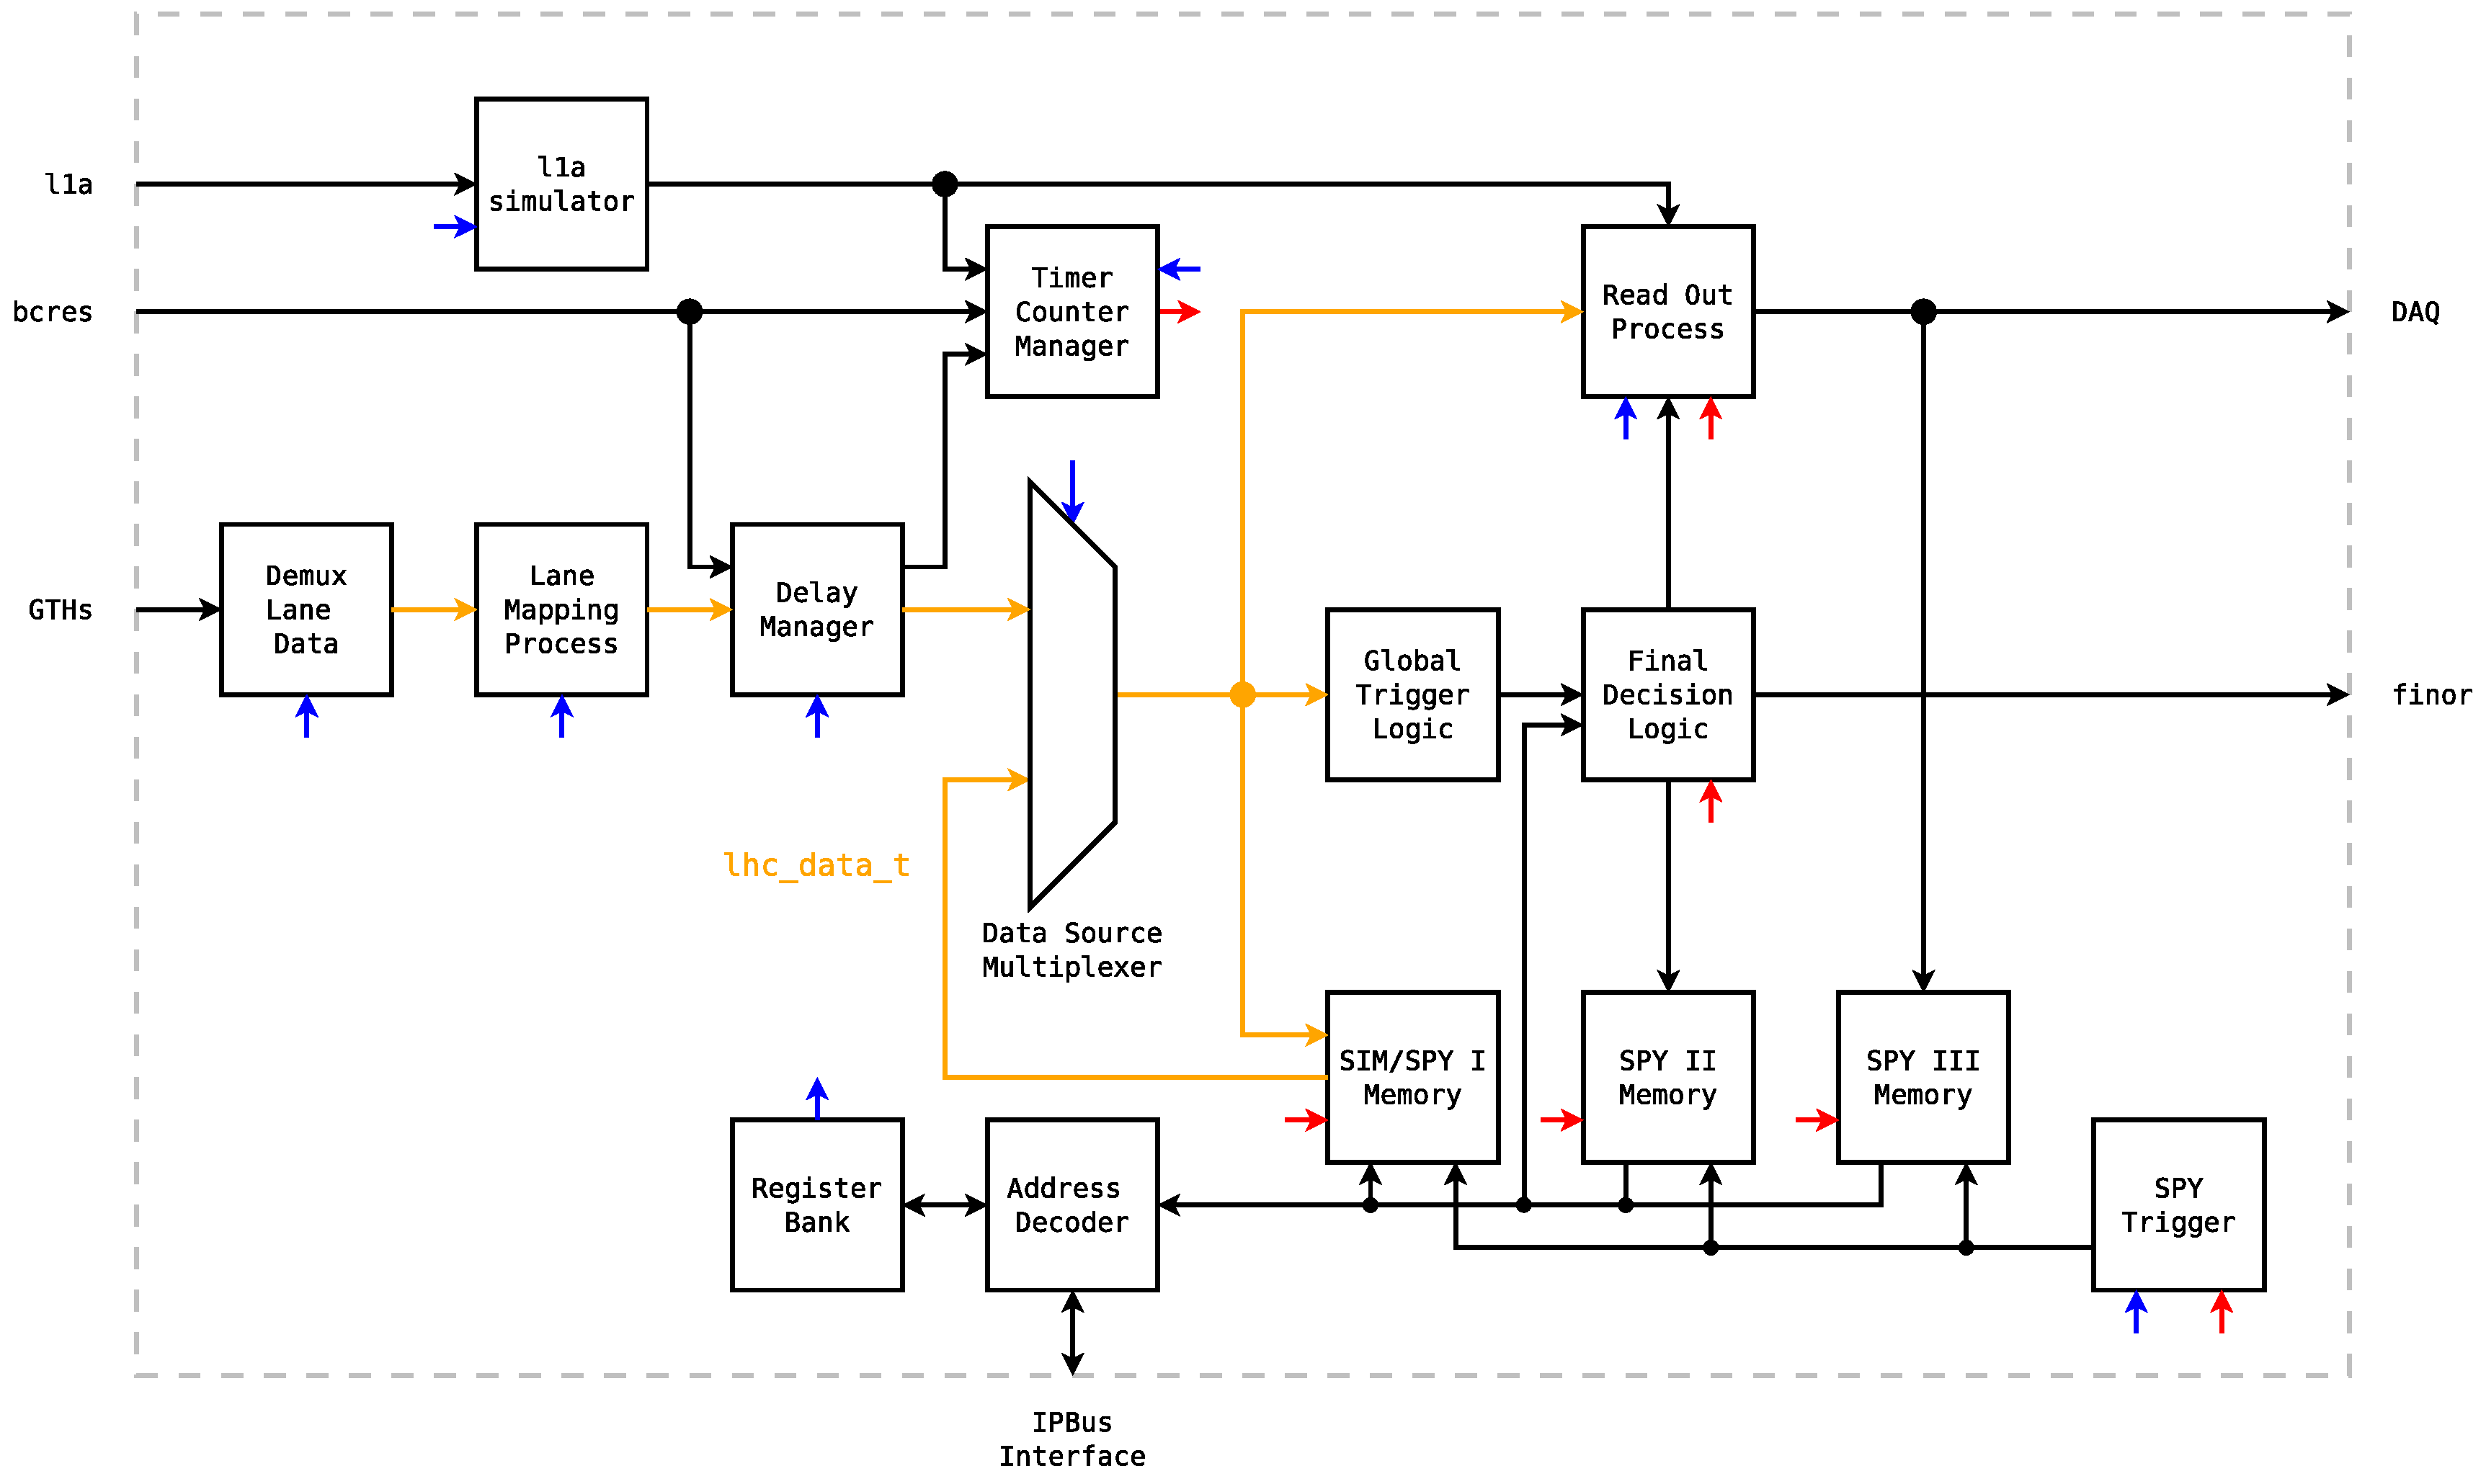
\includegraphics[width=1.0\textwidth]{./figures/system_overview}
\caption{System architecture overview}
\label{fig_system_overview}
\end{figure}

The central data type of the framework is shown in Listing \ref{lst_lhc_data_t} (see Section \ref{section_lhc_data_pkg} for details). In the current configuration it comprises 
2304 bits (288 Bytes). Data from the GTH interfaces is demultiplexed (from 240 MHz clock domain to LHC clock domain, see Demux Lane Data \ref{sec:demux_lane_data}) and mapped to this data type in the LMP (Lane Mapping Process). It is also used as input and output type for the SIM/SPY I memory. 
The DM (Delay Manager) takes the output of the LMP and applies software configurable delays to the the different object streams (e.g. muon data, jet, tau etc.) in the \texttt{lhc\_data\_t} 
to produce a consistent output (also regarding to the bcres signal). The software configurable multiplexer DSMUX (Data Source Multiplexer) is used to select which data stream is used as 
input for the processing elements (trigger logic). The output of the DSMUX is routed to the GTL (Global Trigger Logic) and ROP (Read Out Process) and can optionally be stored in the SPY I memory.

\subsection{Configuration of optical connections} \label{sec:sec_configuration_optical_conn}
The configuration of the optical connections to Calo-Layer2 is (currently) done as described in Table~\ref{tab:framework:tab_configuration_optical_conn}, where
frame means the 32 bits data (240 MHz) within a LHC clock period. 

% \begin{table}[htdp]
% \vspace{5mm}
% \begin{center}
% \begin{tabular}{|c|m{.13\columnwidth}|m{.13\columnwidth}|m{.13\columnwidth}|m{.13\columnwidth}|m{.13\columnwidth}|m{.13\columnwidth}|}
% % \begin{tabular}{|p{.04\columnwidth}|p{.13\columnwidth}|p{.13\columnwidth}|p{.13\columnwidth}|p{.13\columnwidth}|p{.13\columnwidth}|p{.13\columnwidth}|}\hline
% % \begin{tabular}{|c|c|c|c|c|c|c|}\hline
% % \textbf{lane nr} & \textbf{1\textsuperscript{st}} & \textbf{2\textsuperscript{nd}} & \textbf{3\textsuperscript{rd}} & \textbf{4\textsuperscript{th}} & \textbf{5\textsuperscript{th}} & \textbf{6\textsuperscript{th}} \\\hline\hline
% \cline{2-7}
% & \multicolumn{6}{ c| }{\textbf{frame}} \\\hline
% % \textbf{link} & \makebox [.13\columnwidth][c]{\textbf{frame}} & \makebox [.13\columnwidth][c]{\textbf{frame}} & \makebox [.13\columnwidth][c]{\textbf{frame}} & \makebox [.13\columnwidth][c]{\textbf{frame}} & \makebox [.13\columnwidth][c]{\textbf{frame}} & \makebox [.13\columnwidth][c]{\textbf{frame}} \\
% \textbf{link} & \makebox [.13\columnwidth][c]{\textbf{0}} & \makebox [.13\columnwidth][c]{\textbf{1}} & \makebox [.13\columnwidth][c]{\textbf{2}} & \makebox [.13\columnwidth][c]{\textbf{3}} & \makebox [.13\columnwidth][c]{\textbf{4}} &\makebox [.13\columnwidth][c]{\textbf{5}} \\\hline\hline
% 0 & reserved & reserved & muon obj. 0 [0..31] & muon obj. 0 [32..63] & muon obj. 1 [0..31] & muon obj. 1 [32..63]\\\hline
% 1 & reserved & reserved & muon obj. 2 [0..31] & muon obj. 2 [32..63] & muon obj. 3 [0..31] & muon obj. 3 [32..63]\\\hline
% 2 & reserved & reserved & muon obj. 4 [0..31] & muon obj. 4 [32..63] & muon obj. 5 [0..31] & muon obj. 5 [32..63]\\\hline
% 3 & reserved & reserved & muon obj. 6 [0..31] & muon obj. 6 [32..63] & muon obj. 7 [0..31] & muon obj. 7 [32..63]\\\hline
% 4 & \egamma obj. 0 & \egamma obj. 1 & \egamma obj. 2 & \egamma obj. 3 & \egamma obj. 4 & \egamma obj. 5 \\\hline
% 5 & \egamma obj. 6 & \egamma obj. 7 & \egamma obj. 8 & \egamma obj. 9 & \egamma obj. 10 & \egamma obj. 11 \\\hline
% 6 & jet obj. 0 & jet obj. 1 & jet obj. 2 & jet obj. 3 & jet obj. 4 & jet obj. 5 \\\hline
% 7 & jet obj. 6 & jet obj. 7 & jet obj. 8 & jet obj. 9 & jet obj. 10 & jet obj. 11 \\\hline
% 8 & tau obj. 0 & tau obj. 1 & tau obj. 2 & tau obj. 3 & tau obj. 4 & tau obj. 5 \\\hline
% 9 & tau obj. 6 & tau obj. 7 & tau obj. 8 & tau obj. 9 & tau obj. 10 & tau obj. 11 \\\hline
% 10 & \ett, ETTEM, MBT0HFP & \htt, TOWERCOUNT, MBT0HFM & \etm, MBT1HFP & \htm, MBT1HFM & \etm\_HF & \htm\_HF (preliminary definition) \\\hline
% 11 & free & free & free & free & free & free \\\hline
% 12 & external-conditions [0..31] & external-conditions [32..63] & reserved & reserved & reserved & reserved \\\hline
% 13 & external-conditions [64..95] & external-conditions [96..127] & reserved & reserved & reserved & reserved \\\hline
% 14 & external-conditions [128..159] & external-conditions [160..191] & reserved & reserved & reserved & reserved \\\hline
% 15 & external-conditions [192..223] & external-conditions [224..255] & reserved & reserved & reserved & reserved \\\hline
% \end{tabular}
% \end{center}
% \caption{Configuration of optical connections}
% \label{tab:framework:tab_configuration_optical_conn}
% \end{table}

\begin{table}[htdp]
\vspace{5mm}
\begin{center}
\begin{tabular}{c|m{.13\columnwidth}|m{.13\columnwidth}|m{.13\columnwidth}|m{.13\columnwidth}|m{.13\columnwidth}|m{.13\columnwidth}|}
\cline{2-7}
 & \multicolumn{6}{c|}{\textbf{frame}} \\\hline
\multicolumn{1}{|c|}{\textbf{link}} & \makebox[.13\columnwidth][c]{\textbf{0}} & \makebox[.13\columnwidth][c]{\textbf{1}} & \makebox[.13\columnwidth][c]{\textbf{2}} & \makebox[.13\columnwidth][c]{\textbf{3}} & \makebox[.13\columnwidth][c]{\textbf{4}} &\makebox[.13\columnwidth][c]{\textbf{5}} \\\hline\hline
\multicolumn{1}{|c|}{0} & reserved & reserved & muon obj. 0 [0..31] & muon obj. 0 [32..63] & muon obj. 1 [0..31] & muon obj. 1 [32..63]\\\hline
\multicolumn{1}{|c|}{1} & reserved & reserved & muon obj. 2 [0..31] & muon obj. 2 [32..63] & muon obj. 3 [0..31] & muon obj. 3 [32..63]\\\hline
\multicolumn{1}{|c|}{2} & reserved & reserved & muon obj. 4 [0..31] & muon obj. 4 [32..63] & muon obj. 5 [0..31] & muon obj. 5 [32..63]\\\hline
\multicolumn{1}{|c|}{3} & reserved & reserved & muon obj. 6 [0..31] & muon obj. 6 [32..63] & muon obj. 7 [0..31] & muon obj. 7 [32..63]\\\hline
\multicolumn{1}{|c|}{4} & \egamma obj. 0 & \egamma obj. 1 & \egamma obj. 2 & \egamma obj. 3 & \egamma obj. 4 & \egamma obj. 5 \\\hline
\multicolumn{1}{|c|}{5} & \egamma obj. 6 & \egamma obj. 7 & \egamma obj. 8 & \egamma obj. 9 & \egamma obj. 10 & \egamma obj. 11 \\\hline
\multicolumn{1}{|c|}{6} & jet obj. 0 & jet obj. 1 & jet obj. 2 & jet obj. 3 & jet obj. 4 & jet obj. 5 \\\hline
\multicolumn{1}{|c|}{7} & jet obj. 6 & jet obj. 7 & jet obj. 8 & jet obj. 9 & jet obj. 10 & jet obj. 11 \\\hline
\multicolumn{1}{|c|}{8} & tau obj. 0 & tau obj. 1 & tau obj. 2 & tau obj. 3 & tau obj. 4 & tau obj. 5 \\\hline
\multicolumn{1}{|c|}{9} & tau obj. 6 & tau obj. 7 & tau obj. 8 & tau obj. 9 & tau obj. 10 & tau obj. 11 \\\hline
\multicolumn{1}{|c|}{\multirow{3}{*}{10}} & 
\multicolumn{1}{l|}{\ett} & \htt & \etm & \htm & ET$_{miss}^{HF}$ & HT$_{miss}^{HF}$ \\
\multicolumn{1}{|c|}{} &
\multicolumn{1}{l|}{ETTEM} & TOWER-COUNT & ASYMET & ASYMHT & ASYM-ETHF & ASYM-HTHF \\
\multicolumn{1}{|c|}{} &
\multicolumn{1}{l|}{MBT0HFP} & MBT0HFM & MBT1HFP & MBT1HFM & CENT[3:0] & CENT[7:4] \\\hline
\multicolumn{1}{|c|}{11} & free & free & free & free & free & free \\\hline
\multicolumn{1}{|c|}{12} & external-conditions [0..31] & external-conditions [32..63] & reserved & reserved & reserved & reserved \\\hline
\multicolumn{1}{|c|}{13} & external-conditions [64..95] & external-conditions [96..127] & reserved & reserved & reserved & reserved \\\hline
\multicolumn{1}{|c|}{14} & external-conditions [128..159] & external-conditions [160..191] & reserved & reserved & reserved & reserved \\\hline
\multicolumn{1}{|c|}{15} & external-conditions [192..223] & external-conditions [224..255] & reserved & reserved & reserved & reserved \\\hline
\end{tabular}
\end{center}
\caption{Configuration of optical connections}
\label{tab:framework:tab_configuration_optical_conn}
\end{table}

%------------------------------------------------------------------------------
%
%  Demux Lane data
%
% ------------------------------------------------------------------------------

\subsection{Demux Lane Data} \label{sec:demux_lane_data}
Data from GTH interfaces is in the 240 MHz clock domain. The demultiplexing to the LHC clock domain (about 40 MHz) is done in demux\_lane\_data.vhd, which is instantiated
in frame.vhd as often as lanes are used (currently 16 lanes are used). 

%------------------------------------------------------------------------------
%
%  Lane Mapping Process
%
% ------------------------------------------------------------------------------

\subsection{Lane Mapping Process} \label{sec:lmp}
In the Lane Mapping Process module data from the lanes are mapped to objects structure defined in lhc\_data\_pkg.vhd.

\subsubsection{Implementation}\label{sec:lmp_impl}
Currently lane mapping is "fixed" in lmp.vhd module, see Table \ref{tab:framework:current_lane_mapping}

\begin{table}[htdp]
\vspace{5mm}
\begin{center}
\begin{tabular}{|c|l|c|}\hline
\textbf{lane} & \textbf{objects} \\\hline\hline
0 & muon objects 0..1 \\\hline
1 & muon objects 2..3 \\\hline
2 & muon objects 4..5 \\\hline
3 & muon objects 6..7 \\\hline
4 & \egamma objects 0..5 \\\hline
5 & \egamma objects 6..11 \\\hline
6 & jet object 0..5 \\\hline
7 & jet object 6..11 \\\hline
8 & tau object 0..5 \\\hline
9 & tau object 6..11 \\\hline
10 & \esums (incl. minimum bias trigger bits and towercounts) \\\hline
11 & n/a (currently not used) \\\hline
12 & external-conditions [0..63] \\\hline
13 & external-conditions [64..127] \\\hline
14 & external-conditions [128..191] \\\hline
15 & external-conditions [192..255] \\\hline
\end{tabular}
\end{center}
\caption{Current lane mapping}
\label{tab:framework:current_lane_mapping}
\end{table}

%------------------------------------------------------------------------------
%
%  Delay Manager
%
% ------------------------------------------------------------------------------

\subsection{Delay Manager} \label{sec:dm}
\textbf{Remark:}\\
with frame v1.2.3 "Delay Manager" (dm.vhd) and "Data Source Multiplexer" (dsmux.vhd) is removed because these features were never used in production system, only for tests.
The reason of removing is to get more available resources.\\

The Delay Manager is responsible for creating a delayed version of the \texttt{lhc\_data} and the bcres signal on its input. 
For this purpose it uses an internal memory to record the history of the input signals.

\subsubsection{Implementation}\label{sec:dm-impl}
The DM is basically a reimplementation of the concept of the last design. The reimplementation was necessary because the new framework version uses the register bank for 
software registers and the old DM was not flexible enough to handle the \texttt{lhc\_data\_t} introduced in the new framework.

The DM instantiates one \texttt{delay\_element} for every object type defined in the \texttt{lhc\_data\_t} (e.g. muon, eg, etc.). The \texttt{delay\_element} uses RAM blocks 
to implement the delay line. However, for the delays 0 and 1 this memory can not be used (write latency) and must be bypassed (Figure \ref{fig_dm_delay_element}).

\begin{figure}[h]
\begin{center}
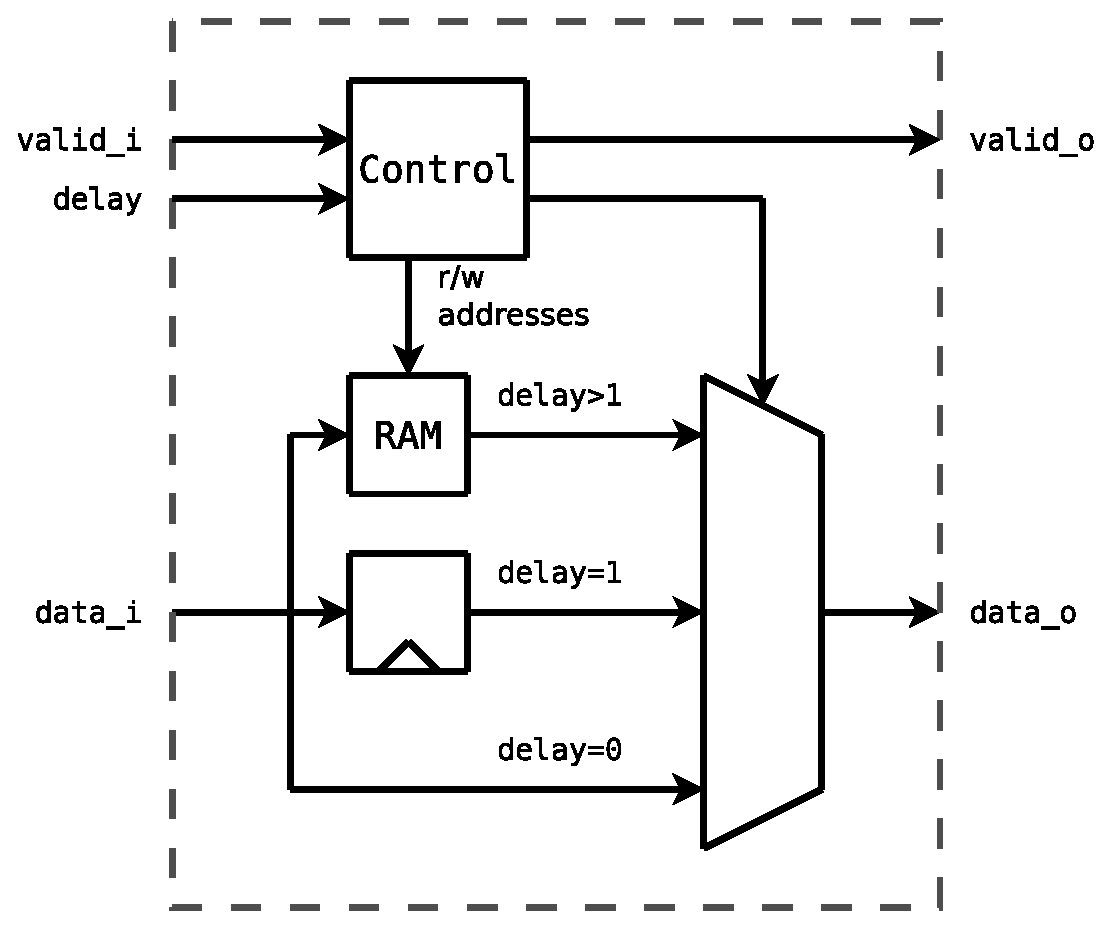
\includegraphics[width=0.5\textwidth]{./figures/dm_delay_element}
\end{center}
\caption{Delay Manager: delay\_element}
\label{fig_dm_delay_element}
\end{figure}

The Implementation of the DM is very generic because it makes extensive use of the constants provided by the \texttt{lhc\_data\_pkg}. The $lhc\_data\_i$ input signal 
is converted into a \texttt{std\_logic\_vector}.
The constants \texttt{LHC\_DATA\_SLV\_START\_INDICES} and \texttt{LHC\_DATA\_SLV\_OBJECT\_WIDTH} provide the start index of each object in this vector and their 
width respectively. The number of objects is given by the \texttt{LHC\_DATA\_OBJECT\_COUNT} constant. This information is used by a for-generate statement to instantiate 
the required \texttt{delay\_element} components.

For the $bcres\_o$ and the $bcres\_FDL\_o$ signals two additional \texttt{delay\_element} components are instantiated. 

If only the data width or the array size of an object in the \texttt{lhc\_data\_t} is changed the DM does not need any modification. If, however, a new object is added a 
new delay register must be added, as described in the register bank section. 

The registers for all delays have the same layout (see Register \ref{dm_reg}). The names for the individual (per object) delay registers are given in Table \ref{tab_dm_regs}. 
For the software addresses of these registers refer to the \texttt{xml/gt\_amc514\_dm.xml} file.

\begin{register}{htbp}{Delay Manager Registers}{}% name=CONFIG
	\label{dm_reg}
	\regfield{reserved}{20}{12}{0}%
	\regfield{delay}{12}{0}{0}%
	\begin{regdesc}
	\begin{reglist}[Request~Depth]
		\item [delay] The delay in lhc clock cycles (40 MHz) used for the specific object data.
	\end{reglist}
	\end{regdesc}
\end{register}

\begin{table}[h]
\vspace{5mm}
\begin{center}
\begin{tabular}{|c|c|}
\hline
object description & register name \\ \hline  \hline
bcres for TCM & bcres\_tcm\_delay \\ \hline
bcres for FDL & bcres\_fdl\_delay  \\ \hline
muon data & muons\_delay  \\ \hline
e/g & eg\_delay  \\ \hline
tau & tau\_delay \\ \hline
jet & jet\_delay  \\ \hline
ett & ett\_delay  \\ \hline
ht & ht\_delay  \\ \hline
etm & etm\_delay  \\ \hline
htm & htm\_delay  \\ \hline
external conditions & ex\_con\_delay  \\ \hline
\end{tabular}
\end{center}
\caption{delay manager registers}
\label{tab_dm_regs}
\end{table}

% \subsubsection{Interface Specification}\label{sec:dm-inter}
% \begin{minipage}{\textwidth}
% \lstinputlisting[language=VHDL,caption=DM interface specification]{interfaces/dm.vhd}
% \end{minipage}
% 
%------------------------------------------------------------------------------
%
%  SIM and SPY Memory
%
% ------------------------------------------------------------------------------

\subsection{SIM and SPY Memory}\label{sec:sim-spy}
\textbf{Remark:}\\
with frame v1.2.3 Simmem data not useable anymore, because of removed "Data Source Multiplexer".
The reason of removing "Data Source Multiplexer" is to get more available resources.\\

\textbf{\textit{Under construction!!!}}

Figure \ref{fig_simspy} shows the SIM/SPY memory subsystem of the framework. 
It is used to calibrate the system, i.e. to set the correct delays in the \hyperref[sec_dm]{Delay Manager}, to record results of the GTL/FDL and 
output packages of the \hyperref[sec_rop]{ROP} and to provide simulation data for the system.
All source files for the memory subsystem are located in \texttt{src/mem} directory. 

\subsubsection{Implementation}\label{sec:sim_spy_impl}
The memory subsystem consists of four main parts, which will be discussed in more detail in the following sections

\begin{itemize}
\item SPY Trigger
\item SIM/SPY Memory
\item SPY Memory II
\item SPY Memory III
\end{itemize}

\begin{figure}[h]
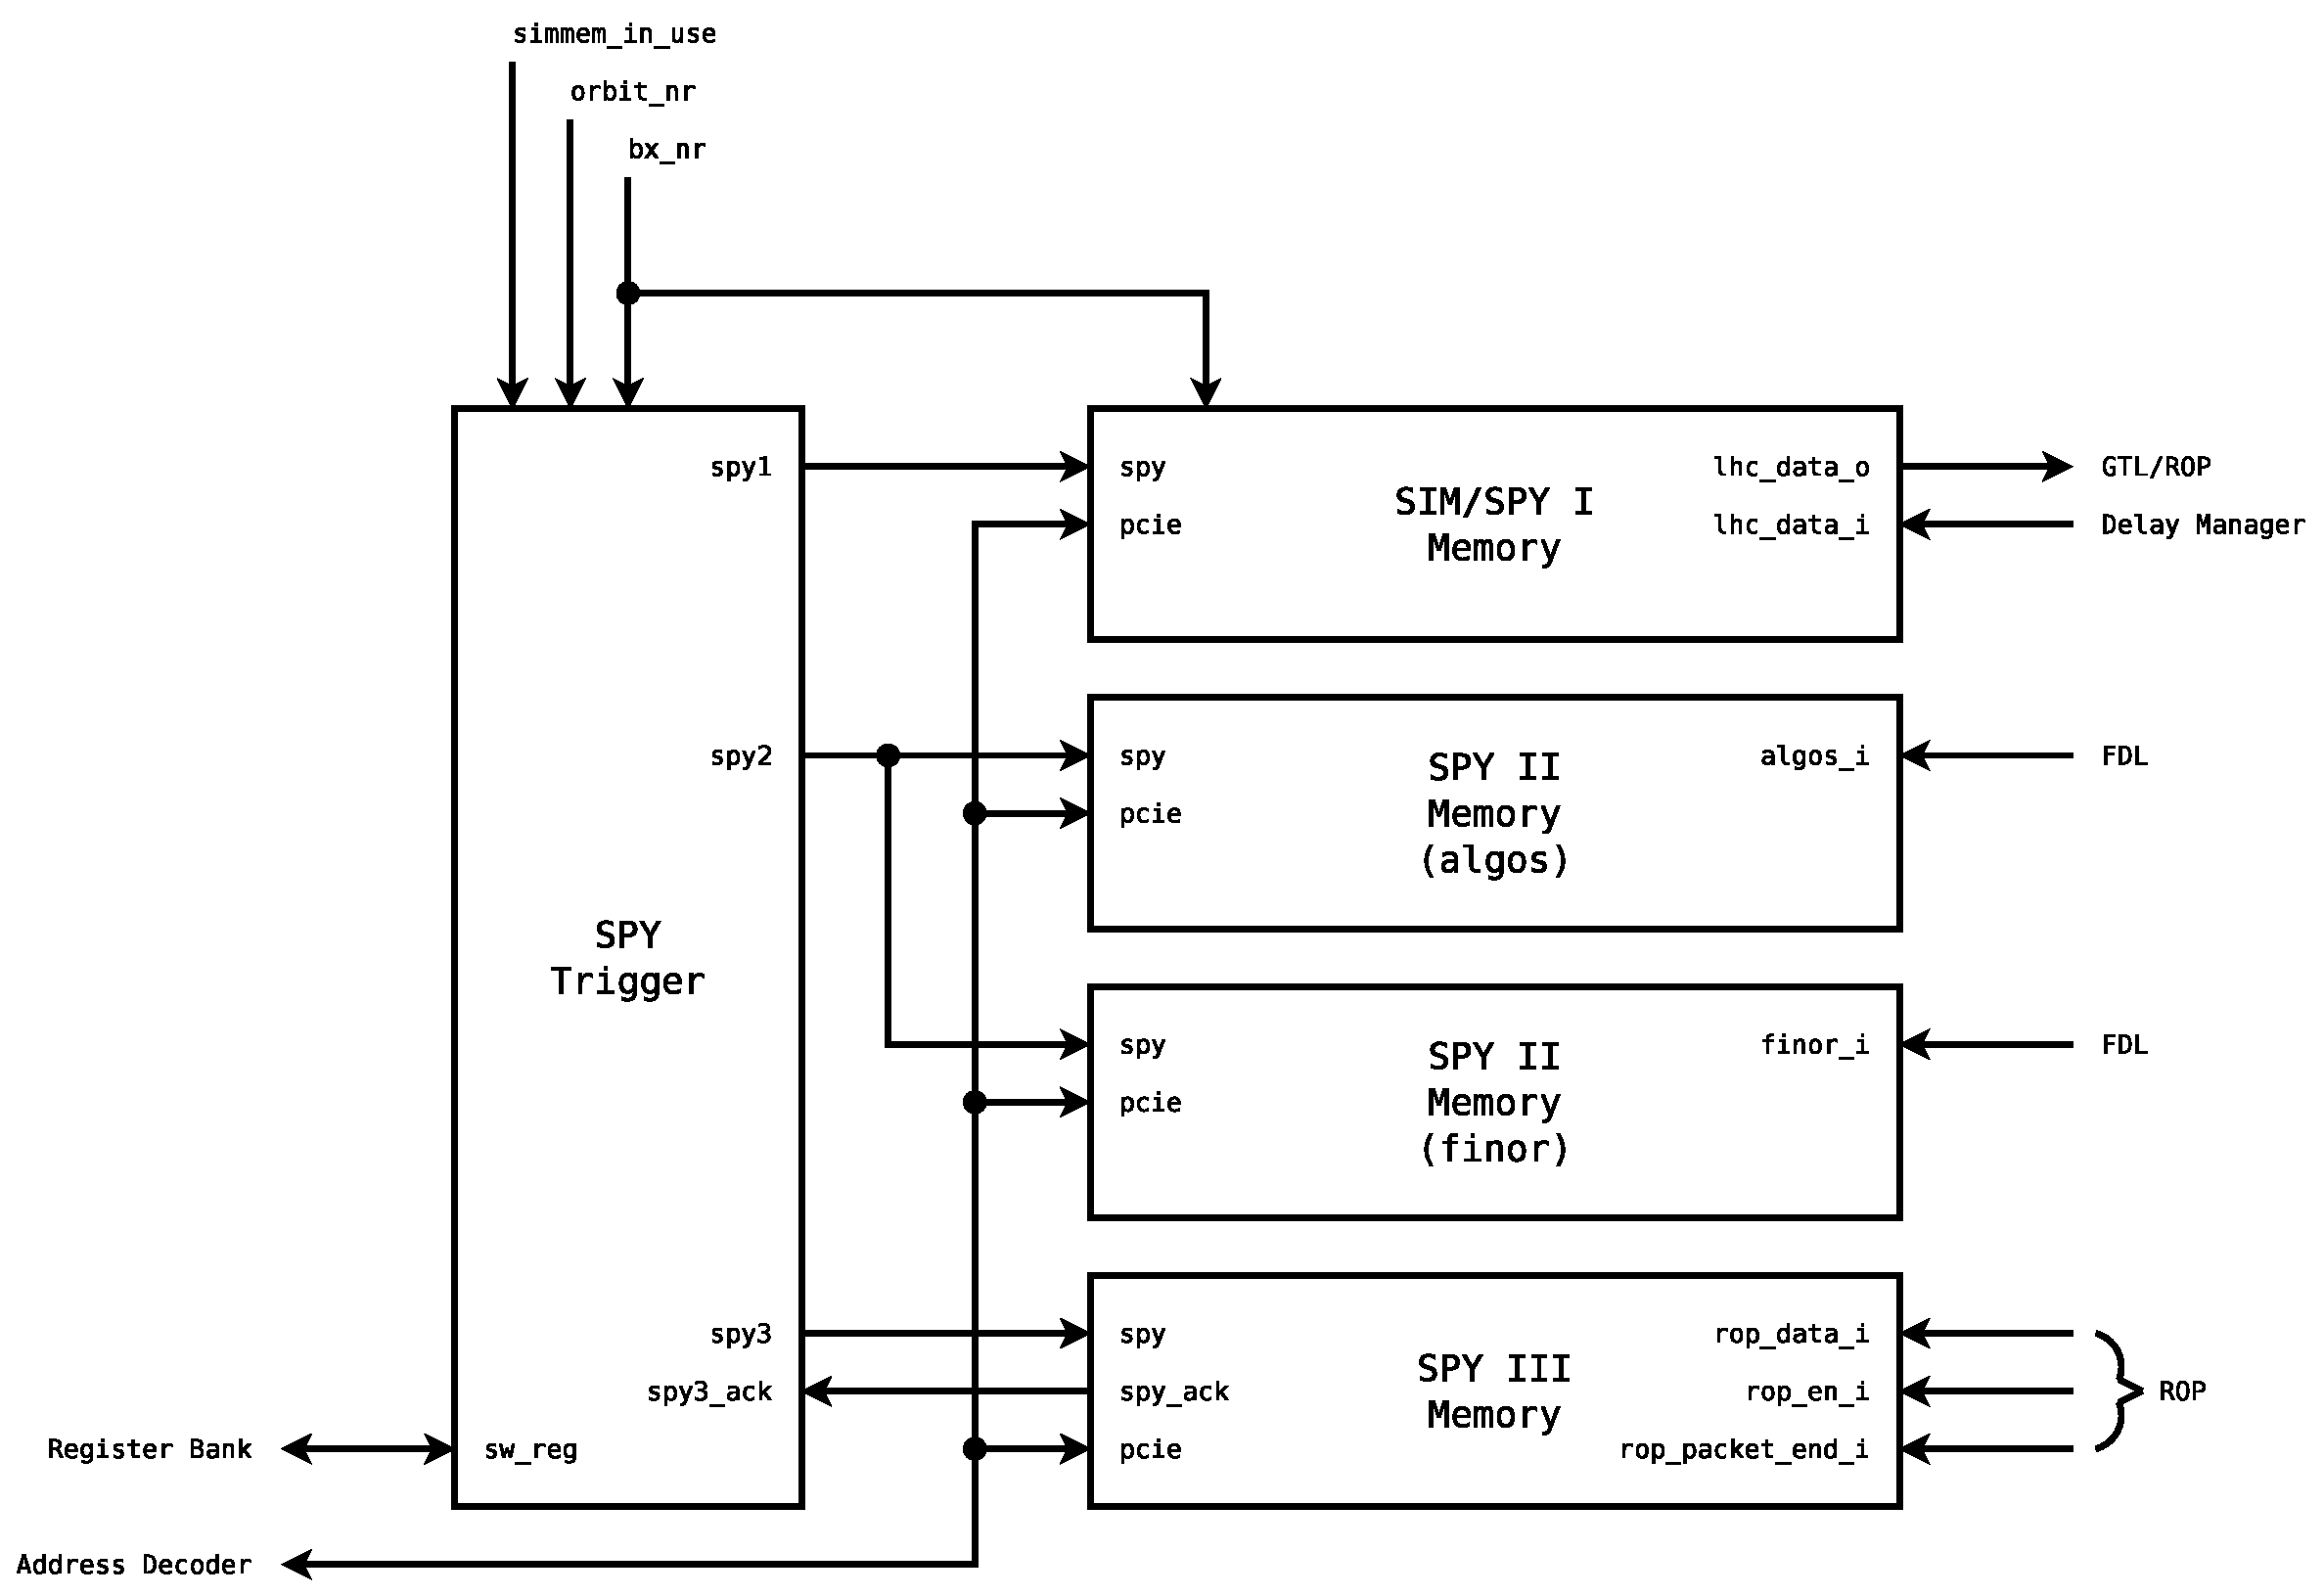
\includegraphics[width=1.0\textwidth]{./figures/simspy}
\caption{Memory subsystem}
\label{fig_simspy}
\end{figure}

\paragraph{SPY Trigger}\label{sec:spy_trigger}
The SPY trigger controls the SPY memories and decides when data is recorded. It can be configured and controlled using 
software registers \ref{spy_trig_obrit_nr_reg} and \ref{spy_trig_cfg_reg} provided by the \hyperref[sec_rb]{register bank}.

\begin{register}{htbp}{SPY Trigger Orbit Number Registers}{}% name=CONFIG
	\label{spy_trig_obrit_nr_reg}
	\regfield{orbit\_nr\_low}{32}{0}{0}%
	\regfield{reserved}{16}{16}{0}%
	\regfield{orbit\_nr\_high}{16}{0}{0}%
	\begin{regdesc}
	\begin{reglist}[Request~Depth]
		\item [orbit\_nr\_low] The 32 low bits of the 48 bit orbit number, used for the spy once trigger.
		\item [orbit\_nr\_high] The 16 high bits of the 48 bit orbit number, used for the spy once trigger.
	\end{reglist}
	\end{regdesc}
\end{register}

\begin{register}{htbp}{SPY Trigger Configuration Register}{}% name=CONFIG
	\label{spy_trig_cfg_reg}%
	\regfield{spy12\_bsy}{1}{31}{0}%
	\regfield{spy3\_bsy}{1}{30}{0}%
	\regfield{spy12\_rdy}{1}{29}{0}%
	\regfield{spy3\_rdy}{1}{28}{0}%
	\regfield{spy12\_err}{1}{27}{0}%
	\regfield{reserved}{21}{6}{0}%
	\regfield{clr\_spy12\_err}{1}{5}{0}%
	\regfield{clr\_spy3\_rdy}{1}{4}{0}%
	\regfield{clr\_spy12\_rdy}{1}{3}{0}%
	\regfield{spy3}{1}{2}{0}%
	\regfield{spy12\_next}{1}{1}{0}%
	\regfield{spy12\_once}{1}{0}{0}%
	\reglabel{Reset}\regnewline%

	\begin{regdesc}
	\begin{reglist}[Request~Depth]
		\item [spy12\_once] Triggers the recording of the selected orbit to SPY memories I and II, when written with 1.
		\item [spy12\_next] Triggers the recording of the next whole orbit to SPY memories I and II, when written with 1.
		\item [spy3] Triggers the recording of the next package that will be sent by the ROP to SPY memory III, when written with 1.
		\item [clr\_spy12\_rdy] Clears the ready flag of the SPY trigger for SPY memories I and II, when written with 1.
		\item [clr\_spy3\_rdy] Clears the ready flag of the SPY trigger for SPY memory III, when written with 1.
		\item [clr\_spy12\_err] Clears the error flag, when written with 1. 
		\item [spy12\_bsy] Indicates that the SPY trigger for SPY memories I and II is busy.
		\item [spy3\_bsy] Indicates that the SPY trigger for SPY memory III is busy.
		\item [spy12\_rdy] Indicates that one orbit has been recorded in SPY memories I and II and that the SPY trigger is ready for new commands.  
		\item [spy3\_rdy] Indicates that packet has been recorded in SPY memory III and that the SPY trigger is ready for new commands. 
		\item [spy12\_err] Indicates an error condition (Set only when the selected orbit number for the spy once trigger lies in the past and can therefore not be recorded).
	\end{reglist}
	\end{regdesc}
\end{register}

When the SPY trigger receives a spy12 command (next or once) over the software register interface it asserts the $spy1$ and $spy2$ signals for the appropriate orbit. 
This means that the $spy$ signals go high with the bunch crossing counter reaching the value zero and stay high until it reaches zero again (overflow). Note that when 
the SIM memory is being used (indicated by the $simem\_in\_use\_i$ input provided by the DSMUX component) the $spy1$ output will not be asserted.

When a spy3 command is received the SPY trigger asserts the $spy3$ signal and waits until the $spy3\_ack$ signal is asserted.

\paragraph{SIM/SPY memory}
This component combines the SIM memory and the SPY memory I. This optimization is possible because these two memories are never used at the same time. There are basically 
two use cases for this memory.
\begin{itemize}
\item SIM memory: Data is read form the memory and provided to GTL and ROP to test these components.
\item SPY memory: External data is received by the GTX and stored in the memory to check the alignment of the data.  
\end{itemize}
It is very important to guarantee that the spy input signal is not asserted, as long as the memory is used as SIM memory. Note that this functionality is implemented in 
the SPY trigger component.

The SIM/SPY memory converts the $lhc\_data\_i$ input signal to a \texttt{std\_logic\_vector} using the converter function provided by the \texttt{lhc\_data\_pkg}. This vector 
is then divided into chunks of 32 bits (the PCIe data width). For each of these chunks a 32 bit true-dual-port memory (2 read ports, 2 write ports, 2 clock domains) is instanciated. 
Thus, every memory has a read/write port in both clock domain, the 125MHz PCIe clock domain and the 40MHz LHC clock domain, which can be used simultaneously.
The PCIe data-in signal ($sw\_i.data$) is connected to PCIe-clock domain write port of the memories. A memory select signal is generated form the LSBs of the software address ($sw\_i.addr$). 
The memory select signal also controls the multiplexer on the output of the memories to generate the $sw\_o.data$ signal.

Depending on whether the SIM/SPY memory is used to provide simulation data or to store/spy data the address on the LHC-clock domain port of the internal memories is adjusted.
If data is recorded (SPY) the bunch crossing counter is used as memory address directly. 
When the memory is read the read latency (two clock cycles) must be taken into account. 
This is achieved by subtracting 2 form the bunch crossing number before using it as address.
To generate the $lhc\_data\_o$ signal the LHC-clock domain data out ports of the internal memories are concatenated and converted back to the \texttt{lhc\_data\_t}.

If the \texttt{lhc\_data\_t} is changed (e.g. new objects added) no modifications in the SIM/SPY memory are required. The SIM/SPY memory only depends on the (auto-generated) 
functions used to convert a \texttt{lhc\_data\_t} signal to \texttt{std\_logic\_vector} and vice versa (see Section \ref{section_lhc_data_pkg} for details).

In the current implementation the size every object in the \texttt{lhc\_data\_t} is a multiple of 32 bit. This is also expected by the SIM/SPY memory. If objects with 16 bit sizes 
are added the SIM/SPY memory must be modified to support this situation (e.g. zero pad the \texttt{lhc\_data\_t}). Furthermore take into account that the PCIe memory bus is 32 bits wide. 
So 16 bit objects should be added to the end of the \texttt{lhc\_data\_t} (as last entry) to keep software memory access simple.

% Table \ref{tab_simpspy} shows the memory layout used to access (read/write) the stored \texttt{lhc\_data\_t}(see Listing \ref{lst_lhc_data_t}). It can be seen that there are areas in 
% the memory that must not be accessed because they do not contain any valid data. 
%require One lhc\_data entry (data for one bunch crossing) needs a memory block 

% \begin{table}[h]
% \begin{center}
% \begin{tabular}{|c|c|}
% \hline
% Address & Data (32 Bit) \\
% (offset from base address) &  \\ \hline
% 0x00000 & BX 0: Muon(0).LOW    \\ \hline
% 0x00001 & BX 0: Muon(0).HIGH   \\ \hline
% 0x00002 & BX 0: Muon(1).LOW    \\ \hline
% 0x00003 & BX 0: Muon(1).HIGH   \\ \hline
% ...    & BX 0: [lhc\_data]    \\ \hline
% 0x00036 & BX 0: External Conditions (7/8) \\ \hline 
% 0x00037 & BX 0: External Conditions (8/8) \\ \hline
% 0x00038 & undefined (do not access) \\ \hline
% ...    & undefined (do not access) \\ \hline
% 0x0003F & undefined (do not access) \\ \hline
% 0x00040 & BX 1: Muon(0).LOW    \\ \hline
% 0x00041 & BX 1: Muon(0).HIGH   \\ \hline
% 0x00042 & BX 1: Muon(1).LOW    \\ \hline
% 0x00043 & BX 1: Muon(1).HIGH   \\ \hline
% ...     & ...       \\ \hline
% 0x37AF7 & BX 3563: External Conditions (8/8)    \\ \hline
% \end{tabular}
% \end{center}
% \caption{SIM/SPY I memory layout}
% \label{tab_simpspy}
% \end{table}
% 
% It is important to note, that the start address of the SIM/SPY memory (configured in the address decoder) must be a multiple of the size of the memory (in the current 
% configuration $2^{18}$ byte addresses).
% To handle/simplify the memory access to this memory special python classes (\verb|GTMemory.py| and \verb|GTMemoryImage.py|) are provided. The XML specification in 
% Listing \ref{lst_lhc_data_t_xml} is used to obtain the memory layout. See the source files for further details and examples of how to use them.

\paragraph{SPY memory II}
The SPY memory II is divided into two subcomponents, to store the $algos$ and $finor$ outputs of the FDL. 
Both memory can only be read over the SW interface. A write access has no effect.
% Tables \ref{tab_spy2_algos} and \ref{tab_spy2_finor} show the memory layout as seen by the software. 
The algos memory uses the same architecture as the SIM memory.
The finor memory uses a true-dual-port memory with asymmetric ports. This memory can be written with a data width of one bit and read with a data width of 32 bit. 

% \begin{table}[h]
% \begin{center}
% \begin{tabular}{|c|c|}
% \hline
% Address & Data (32 Bit) \\
% (offset from base address) &   \\ \hline
% 0x00000 & BX 0: algos: 31-0 (1/16)     \\ \hline
% 0x00001 & BX 0: algos: 64-32 (2/16)    \\ \hline
% ...     & BX 0: ...            \\ \hline
% 0x0000F & BX 0: algos: 511-480 (16/16)   \\ \hline
% 0x00010 & BX 1: algos: 31-0 (1/16)    \\ \hline
% 0x00011 & BX 1: algos: 63-32 (2/16)    \\ \hline
% ...     & BX 1: ...            \\ \hline
% 0x0001F & BX 1: algos: 511-480 (16/16)  \\ \hline
% ...\\ \hline
% 0x0DEBF & BX 3563: algos: 511-480 (16/16)\\ \hline
% \end{tabular}
% \end{center}
% \caption{SPY II algos memory layout}
% \label{tab_spy2_algos}
% \end{table}
% 
% 
% \begin{table}[h]
% \begin{center}
% \begin{tabular}{|c|c|}
% \hline
% Address & Data (32 Bit) \\
% (offset from base address) &   \\ \hline
% 0x00000 & finor for BX 31-0      \\ \hline
% 0x00001 & finor for BX 64-32     \\ \hline
% ...
% 0x00070 & BX 3563: algos: 3552-3563 \\ \hline
% \end{tabular}
% \end{center}
% \caption{SPY II finor memory layout}
% \label{tab_spy2_finor}
% \end{table}
% 
% Note that the start addresses of the algos and finor memories (configured in the address decoder) must be a multiples of their sizes (in the current configuration $2^{16}$ and $2^7$).  
%  
\paragraph{SPY memory III}
The SPY memory III stores the output of the ROP, which is sent to the DAQ. The input data width is configurable to bus widths of 16, 32 or 64 bits.
Depending on the input data width the memory uses different architectures.
\begin{itemize} 
\item 16 Bit \\
A true-dual-port memory with asymmetric ports (16 and 32 bits) is used. 
\item 32 Bit \\
A true-dual-port memory with 32 Bit data width is used.
\item 64 Bit \\
Two true-dual-port memories with 32 Bit data width are used.
\end{itemize}

% \subsubsection{Software}
% The \texttt{gtamc514-memdump} python script can be used to access/read all spy memories of the system.  The \texttt{gtamc514-simmem} script is used to write 
% data to the SIM memory. Refer to See \texttt{gtamc514-memdump -h} and \texttt{gtamc514-simmem -h} for further details.
% 
\subsubsection{Interface Specification}

\begin{minipage}{\textwidth}
\lstinputlisting[language=VHDL,caption=SPY trigger interface specification]{interfaces/spytrig.vhd}
\end{minipage}

% \begin{minipage}{\textwidth}
% \lstinputlisting[language=VHDL,label=lst_simspymem,caption=SIM/SPY I memory interface specification]{interfaces/simspymem.vhd}
% \end{minipage}
% 
% \begin{minipage}{\textwidth}
% \lstinputlisting[language=VHDL,caption=SPY memory II (algos) interface specification]{interfaces/spymem2_algos.vhd}
% \end{minipage}
% 
% \begin{minipage}{\textwidth}
% \lstinputlisting[language=VHDL,caption=SPY memory II (finor) interface specification]{interfaces/spymem2_finor.vhd}
% \end{minipage}
% 
% \begin{minipage}{\textwidth}
% \lstinputlisting[language=VHDL,caption=SPY memory III interface specification]{interfaces/spymem3.vhd}
% \end{minipage}
% 
%------------------------------------------------------------------------------
%
%  L1A Simulator
%
% ------------------------------------------------------------------------------
% \subsection{L1A Simulator}
% 
% The simulation component for the l1a signal has been reimplemented based on specification of the last semester.
% 
% The L1A SIM/MUX module takes as input the synchronized real l1a signal (usually originating from the TCS) and outputs depending on its configuration the (undelayed) real l1a signal or a simulation of the signal. The following simulation modes which are configurable through software register access are available:
% \begin{itemize}
% \item fire once: the l1a signal is set to high for exactly one clock cycle as soon as the software
% register access has been issued. Note that this mode overrides both, the real l1a and
% any simulation mode. After the single l1a event completed, the L1A SIM/MUX module
% continues operation according to the sim\_mode register.
% \item pattern at orbit: replay a predefined l1a pattern at a specified orbit counter value.
% \item alternating patterns: replay a predefined l1a pattern at an even orbit counter value,
% followed by another predefined l1a pattern at an odd orbit counter value. This mode
% is freerunning: the two orbit patterns are replayed in an alternating way as long as the
% mode is active.
% \end{itemize}
% A l1a pattern consists of bunch crossing number (bx\_nr) compare values that indicate
% when exactly the simulated l1a signal is supposed to be active (set to high). As the maximum
% frequency of l1a signal occurrences is 100 kHz (10 l1a events per orbit), a l1a pattern
% consists of 10 such bunch crossing counter compare values. Not all of the 10 places need to be
% used: in case a bunch crossing counter compare value is higher than BUNCHES\_PER\_ORBIT-1
% (e.g. 0xdec), but lower than 0x1000, it is ignored. Alternatively unused places can also be
% set to values that are already specified.
% Through software register access 2 l1a pattern can be specified: pattern A and pattern B. For
% the first mode (fire once) no pattern is considered, for the second mode (pattern at orbit), only
% pattern A is used and for the last mode (alternating patterns), pattern A (even orbits) and
% pattern B (odd orbits) are used. In case both, the second and the third mode are activated
% by software register access, the third mode overrides the second one.
%  
% Registers \ref{l1asim_cfg_reg} \ref{l1asim_orbit_nr_reg} \ref{l1asim_pattern_reg} specify the software interface.
% 
% \begin{register}{htbp}{L1A Simulator Configuration Register}{}% name=CONFIG
% 	\label{l1asim_cfg_reg}%
% 	\regfield{reserved}{28}{4}{0}%
% 	\regfield{sim\_mode}{2}{2}{0}%
% 	\regfield{fire\_once}{1}{1}{0}%
% 	\regfield{enable\_sim}{1}{0}{0}%
% 	\reglabel{Reset}\regnewline%
% 
% 	\begin{regdesc}
% 	\begin{reglist}[Request~Depth]
% 			\item [enable\_sim] Enables the l1a simulation module. This bit must be 1 for all other configurations to have an effect. If this bit is zero the real l1a signal is presented at the output of the l1asim module.
% 			\item [fire\_once] When written with 1, triggers one l1a event as soon as the hardware recognizes the register access (It is not possible to exactly time the event using this trigger)
% 			\item [sim\_mode] Selects one of the two simulation modes (pattern at orbit, alternating patterns). If zero (00) no mode is selected. 
% 	\end{reglist}
% 	\end{regdesc}
% \end{register}
% 
% \begin{register}{htbp}{L1A Simulator Orbit Number Registers}{}% name=CONFIG
% 	\label{l1asim_orbit_nr_reg}
% 	\regfield{orbit\_nr\_low}{32}{0}{0}%
% 	\regfield{reserved}{16}{16}{0}%
% 	\regfield{orbit\_nr\_high}{16}{0}{0}%
% 	\begin{regdesc}
% 	\begin{reglist}[Request~Depth]
% 		\item [orbit\_nr\_low] The 32 low bits of the 48 bit orbit number, used for the pattern at orbit simulation mode.
% 		\item [orbit\_nr\_high] The 16 high bits of the 48 bit orbit number, used for the pattern at orbit simulation mode.
% 	\end{reglist}
% 	\end{regdesc}
% \end{register}
% 
% \begin{register}{htbp}{L1A Simulator Pattern Registers}{}% name=CONFIG
% 	\label{l1asim_pattern_reg}
% 	\regfield{reserved}{20}{12}{0}%
% 	\regfield{bx\_nr}{12}{0}{0}%
% 	\begin{regdesc}
% 	\begin{reglist}[Request~Depth]
% 		\item [bx\_nr] The 12 bit bunch crossing number, used for the pattern at orbit and the alternating patterns simulation mode. Currently there are 10 pattern registers available (l1asim\_pattern\_a[0-4] and l1asim\_pattern\_b[0-4])
% 	\end{reglist}
% 	\end{regdesc}
% \end{register}
% 
% \subsubsection{Interface Specification}
% 
% \begin{minipage}{\textwidth}
% \lstinputlisting[language=VHDL,caption=L1A Simulation module interface specification]{interfaces/l1asim.vhd}
% \end{minipage}
% 
%------------------------------------------------------------------------------
%
%  TCM
%
% ------------------------------------------------------------------------------
\subsection{TCM}\label{sec:tcm}
\textbf{\textit{Under construction!!!}}

The Timer Counter Manager (TCM) provides different counters, listed in table \ref{tab:tcm_counters}.

\subsubsection{Counter Overview}
\begin{table}[H]
\vspace{5mm}
\begin{scriptsize}
\begin{tabular}{|l|l|l|l|l|}
\hline
Counter             &range              &increase condition               &reset condition           &Comments     \\ \hline
bx\_nr              &$0 to 3563$        &rising\_edge(lhc\_clk)           &overflow                  &             \\ \hline
event\_nr           &$0 to 2^{32}-1$    &l1a=1 and rising\_edge(lhc\_clk) &BGOS: event counter reset &             \\ \hline
trigger\_nr         &$0 to 2^{48}-1$    &l1a=1 and rising\_edge(lhc\_clk) &BGOS: start run           &             \\ \hline
orbit\_nr           &$0 to 2^{48}-1$    &overflow of bx\_nr               &BGOS: orbit counter reset &             \\ \hline
luminosity\_seg\_nr &$0 to 2^{32}-1$    &rising\_edge(orbit\_nr(18))      &BGOS: orbit counter reset &             \\ \hline
start\_lumisection  &$0 to 1$           &luminosity\_seg\_nr increases    &after 25ns                &'1' for 25ns \\ \hline
bx\_nr\_d\_fdl      &$0 to 3563$       &rising\_edge(lhc\_clk)            &overflow                  &             \\ \hline
\end{tabular}\caption{counters of the timer counter manager}\label{tab:tcm_counters}
\end{scriptsize}
\end{table}

\subsubsection{Bunch Crossing Number and counters derived from it}
All counters except for event\_nr and the trigger\_nr (which are trivial because they are increased with l1a) are dependent on the bunch crossing counter bx\_nr as stated in table \ref{tab:tcm_counters}. The bx\_nr is zero at startup, then waits for the the first bcres\_d (bunch crossing reset delayed) and starts counting as depicted in figure \ref{fig:bx_start}. It's maximal value is 3563 (0xdeb), then it automatically overflows and starts at zero again (see figure \ref{fig:bx_normal_operation}). Exactly when bx\_nr = 0, bcres\_d has to be asserted. Otherwise the counter is out of synchronization. If this happens, the software register err\_det is set and the counter waits for the next bcres\_d to synchronize again. Note that the value of the counter is invalid until it has synchronized again.

\begin{figure}[ht]
  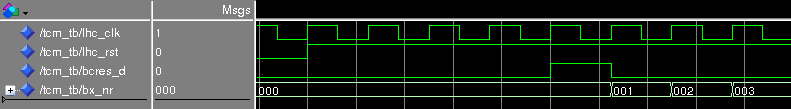
\includegraphics[width=1.0\textwidth]{./figures/bx_start}
  \caption{start of the bunch crossing number with the first bcres\_d}
  \label{fig:bx_start}
\end{figure}

\begin{figure}[ht]
  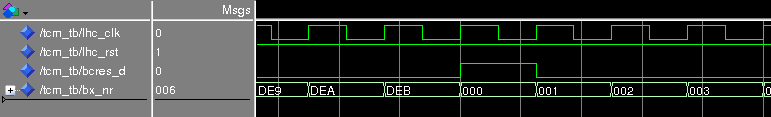
\includegraphics[width=1.0\textwidth]{./figures/bx_normal_operation}
  \caption{normal operation of the bunch crossing number}
  \label{fig:bx_normal_operation}
\end{figure}

\subsubsection{Special counter: bx\_nr\_d\_fdl}
The bx\_nr\_d\_fdl is derived from bcres\_d\_fdl in the same manner as bx\_nr is derived from bcres\_d. bx\_nr\_d\_fdl will automatically resync if the logic described in subsection \ref{subsec:tcmerrors} detects a synchronization error for bx\_nr.

\subsubsection{Counters derived from l1a}
The counters event\_nr and trigger\_nr are increased with l1a, i.e. they are increased twice if l1a is high for 2 clock cycles, etc. They differ only in their value range and the condition that resets the counters, see table \ref{tab:tcm_counters}.

\subsubsection{Errors}\label{subsec:tcmerrors}
As stated above, bcres\_d has to be asserted exactly when bx\_nr = 0, otherwise the counter is out of sync. Then the software register err\_det is set as depicted in figure \ref{fig:err_det}. err\_det can be reset via the software event register err\_det\_reset\_event as depicted in figure \ref{fig:err_det_reset}. Furthermore err\_det is set if bgos = Resync-0x1 and the counter value is not 3563.

\begin{figure}[ht]
  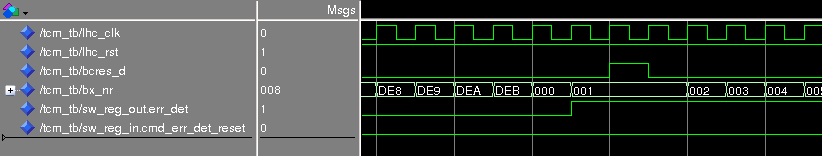
\includegraphics[width=1.0\textwidth]{./figures/err_det}
  \caption{set of the software register err\_det when bc\_res\_d is not asserted correctly}
  \label{fig:err_det}
\end{figure}

\begin{figure}[ht]
  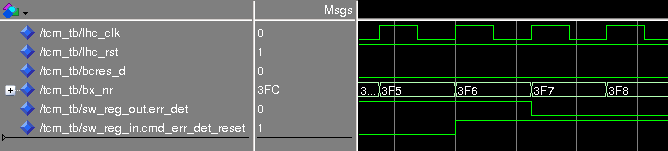
\includegraphics[width=1.0\textwidth]{./figures/err_det_reset}
  \caption{reset of the software register err\_det when err\_det\_reset\_event toggles}
  \label{fig:err_det_reset}
\end{figure}

The TCM implements two additional counters (bx\_nr\_chk and bx\_nr\_max) for debugging purposes. These counters are not visible by any other module but readable via software. bx\_nr\_chk is a 32bit Counter that increases with every LHC clock cycle and resets with bcres\_d. bx\_r\_max holds the highest value bx\_nr\_chk ever reached (should be 3563 if the link is aligned).

\subsubsection{SW-Registers}
All counters except for the start\_lumisection described in table \ref{tab:tcm_counters} can be read by software via the following sw registers:

\begin{register}{H}{TCM Bunch Crossing Number Register}{}%
	\regfield{reserved}{20}{12}{0}%
	\regfield{bx\_nr}{12}{0}{0}%
	\begin{regdesc}
	\end{regdesc}
\end{register}
\begin{register}{H}{TCM Event Number Register}{}%
	\regfield{event\_nr}{32}{0}{0}%
	\begin{regdesc}
	\end{regdesc}
\end{register}
\begin{register}{H}{TCM Trigger Number Registers}{}%
	\regfield{trigger\_nr\_l}{32}{0}{0}%
	\regfield{reserved}{16}{16}{0}%
	\regfield{trigger\_nr\_h}{16}{0}{0}%
	\begin{regdesc}
	\begin{reglist}[Request~Depth]
		\item [trigger\_nr\_l] The 32 low bits of the 48 bit trigger number.
		\item [trigger\_nr\_h] The 16 high bits of the 48 bit trigger number.
	\end{reglist}
	\end{regdesc}
\end{register}
\begin{register}{H}{TCM Orbit Number Registers}{}%
	\regfield{orbit\_nr\_l}{32}{0}{0}%
	\regfield{reserved}{16}{16}{0}%
	\regfield{orbit\_nr\_h}{16}{0}{0}%
	\begin{regdesc}
	\begin{reglist}[Request~Depth]
		\item [orbit\_nr\_l] The 32 low bits of the 48 bit orbit number.
		\item [orbit\_nr\_h] The 16 high bits of the 48 bit orbit number.
	\end{reglist}
	\end{regdesc}
\end{register}
\begin{register}{H}{TCM Luminosity Segment Number Register}{}%
	\regfield{luminosity\_seg\_nr}{32}{0}{0}%
	\begin{regdesc}
	\end{regdesc}
\end{register}
\begin{register}{H}{TCM Bunch Crossing Number FDL Register}{}%
	\regfield{reserved}{20}{12}{0}%
	\regfield{bx\_nr\_d\_fdl}{12}{0}{0}%
	\begin{regdesc}
	\end{regdesc}
\end{register}
\begin{register}{H}{TCM Bunch Crossing Number Check Register}{}%
	\regfield{bx\_nr\_chk}{32}{0}{0}%
	\begin{regdesc}
	\end{regdesc}
\end{register}
\begin{register}{H}{TCM Bunch Crossing Number Max Register}{}%
	\regfield{bx\_nr\_max}{32}{0}{0}%
	\begin{regdesc}
	\end{regdesc}
\end{register}

Some additional control register can be used to check and reset err\_det, disable the check of bcres\_d and bcres\_d\_fdl (bx\_nr and bx\_nr\_d\_fdl automatically reset when they overflow if cmd\_ign\_bcres is set, bcres\_d is ignored) and simulate the bgos signal. To do this, a value of the orbit signal has to be written to sw-register bgos. The value of the input signal bgos is replaced by the value of the sw-register for exactly one clock cycle, when "1" is written to the event register bgos\_event.

\begin{register}{H}{TCM cmd\_ign\_bcres}{}% name=CONFIG
	\label{cmd_ign_bcres}%
 	\regfield{reserved}{31}{1}{0}%
 	\regfield{cmd\_ign\_bcres}{1}{0}{0}%
	\reglabel{Reset}\regnewline%

	\begin{regdesc}
	\begin{reglist}[Request~Depth]
 		\item [cmd\_ign\_bcres] bcres is ignored (not checked) when this is set.
	\end{reglist}
	\end{regdesc}
\end{register}

\begin{register}{H}{TCM err\_det}{}% name=CONFIG
	\label{err_det}%
 	\regfield{reserved}{31}{1}{0}%
	\regfield{err\_det}{1}{0}{0}%
	\reglabel{Reset}\regnewline%

	\begin{regdesc}
	\begin{reglist}[Request~Depth]
		\item [err\_det] Set when out of synchronization.
	\end{reglist}
	\end{regdesc}
\end{register}

\begin{register}{H}{TCM err\_det\_reset\_event}{}% name=CONFIG
	\label{err_det_reset_event}%
 	\regfield{reserved}{31}{1}{0}%
 	\regfield{err\_det\_reset\_event}{1}{0}{0}%
	\reglabel{Reset}\regnewline%

	\begin{regdesc}
	\begin{reglist}[Request~Depth]
 		\item [err\_det\_reset\_event] Event register: resets err\_det.
	\end{reglist}
	\end{regdesc}
\end{register}

\begin{register}{H}{TCM bgos}{}% name=CONFIG
	\label{bgos}%
 	\regfield{reserved}{31}{4}{0}%
 	\regfield{bgos}{4}{0}{0}%
	\reglabel{Reset}\regnewline%

	\begin{regdesc}
	\begin{reglist}[Request~Depth]
 		\item [bgos] For simulation of the bgos signal.
	\end{reglist}
	\end{regdesc}
\end{register}

\begin{register}{H}{TCM bgos\_event}{}% name=CONFIG
	\label{bgos_event}%
 	\regfield{reserved}{31}{1}{0}%
 	\regfield{bgos\_event}{1}{0}{0}%
	\reglabel{Reset}\regnewline%

	\begin{regdesc}
	\begin{reglist}[Request~Depth]
 		\item [bgos\_event] Event register: replaces the input signal bgos by the sw-register bgos for exactly one clock cycle.
	\end{reglist}
	\end{regdesc}
\end{register}

\begin{register}{H}{TCM luminosity\_seg\_period\_msk}{}% name=CONFIG
	\label{luminosity_seg_period_msk}%
 	\regfield{luminosity\_seg\_period\_msk}{32}{0}{0x40000}%
	\reglabel{Reset} %\regnewline%

	\begin{regdesc}
	\begin{reglist}[Request~Depth]
 		\item [luminosity\_seg\_period\_msk] luminosity\_seg\_nr is increased when the orbit\_nr mod lum\_seg\_period\_mask = 0.
	\end{reglist}
	\end{regdesc}
\end{register}

\subsubsection{Hardware Test}
There are various python scripts located in the software/GtControl/branches/fpga-design-2013/python/GtControl directory for testing the tcm module. Please refer to the output of the scripts for information how the tests are performed in detail. See table \ref{tab:tcm_hw_test}.
\begin{table}[ht]
\vspace{5mm}
\begin{scriptsize}
\begin{tabular}{|p{5cm}|p{10cm}|}
\hline
script                         &purpose    \\ \hline
\verb|tcm_counter_values.py|   &outputs the values of all counters defined above    \\ \hline
\verb|tcm_produce_err_det|     &produces an err\_det by manipulating bgos \\ \hline
\verb|tcm_err_det_reset|       &resets the err\_det software register \\ \hline
\verb|tcm_trigger_test|        &tests trigger\_nr and event\_nr by generating l1a signals using l1asim \\ \hline
\verb|tcm_lum_seg_nr_test|    &checks the period of two successive increases of the luminositiy\_seg\_nr \\ \hline
\end{tabular}\caption{scripts for testing the tcm}\label{tab:tcm_hw_test}
\end{scriptsize}
\end{table}

% \subsubsection{Interface}
% 
% \lstinputlisting[language=VHDL,caption=TCM interface specification]{interfaces/tcm.vhd} 

\subsection{Software Reset} \label{sec:software_reset}
The software reset module (sw\_reset) provides the possiblity for a software reset via the software event register sw\_reset\_event.

\begin{register}{htbp}{Software Reset register}{}% name=CONFIG
	\label{tcm_ctrl_reg}%
	\regfield{reserved}{31}{1}{0}%
	\regfield{sw\_reset\_event}{1}{0}{0}%
	\reglabel{Reset}\regnewline%

	\begin{regdesc}
	\begin{reglist}[Request~Depth]
		\item [sw\_reset\_event] Event register: Generates a reset signal for exactly one clock cycle.
	\end{reglist}
	\end{regdesc}
\end{register}

\clearpage







% %------------------------------------------------------------------------------
%
% Repository path   : $HeadURL: https://hbergauer@forge.hephy.oeaw.ac.at/scm/svn/project-cmstrigger/GlobalTriggerUpgrade/doc/latex/gt-mp7-firmware-specification/content/ipbus.tex $
% Last committed    : $Revision: 4338 $
% Last changed by   : $Author: hbergauer $
% Last changed date : $Date: 2016-06-17 08:45:22 +0200 (Fri, 17 Jun 2016) $
% Description       : IPBus Structure: Fabric/Slave
% ------------------------------------------------------------------------------
\section {IPBus}\label{sec:ipbus}
\textbf{\textit{Under construction!!!}}

% For the Gigabit Ethernet links, MAC cores are instantiated. Depending on the compilation settings,
% one or two Gigabit Ethernet Links are instantiated (for bench-top and crate operation respectively).
% In the case of bench-top operation, the MAC core is configured as 1000Base-T in order to
% communicate with the external PHY. In the case of crate operation, both MAC cores are configured
% as 1000Base-X for interfacing with the Gigabit Ethernet Switch carried on th
% e crate’s MCH.
% For every MAC core, an IPbus endpoint is also instantiated. The IPBus system allows the control of
% hardware via a ‘virtual bus’, using a standard IP-over-gigabit-Ethernet network connection. The
% IPBus specifies a simple transaction protocol between the hardware and a software controller, which
% assumes an A32/D32 connection to slave devices connected to the hardware endpoint. The current
% IPbus firmware implementation is using a UDP/IP protocol and a simple synchronous SoC bus.
% 
% This protocol is based upon the Wish bone SoC protocol, and is compatible with Wishbone
% cores. However, there are two important differences:
% \begin{itemize}
%  \item The master is not required to explicitly deassert strobe between cycles. However, it is guaranteed to deassert strobe or begin the new cycle 
%  on the clock cycle following ack. 
% \item Slaves are not al lowed to tie ack high, and must deassert ack on the same clock cycle that strobe is
% deasserted. However, it is allowed to tie ack to strobe, if a zero-wait-state response is always possible.
% \end{itemize}
% 
% \subsection{Implementation}\label{sec:ad-impl}
% under construction ...
% 
% \subsection{Interface}\label{sec:ad-interface}
% 
% %\lstinputlisting[language=VHDL,caption=AD interface specification]{interfaces/ad.vhd} 
% 
% \subsection{How to use registers} \label{subsec:UseRegisters}
% \subsection{How to add Slaves/Fabric} \label{subsec:addRegisters}
% %The following document should be integrated in this chapter:
% %1) IPbus Network Architecture for μTCA Hardware:https://svnweb.cern.ch/trac/cactus/browser/trunk/doc/uHAL_etwork_addressing.docx
% %2) The IPbus Protocol: https://svnweb.cern.ch/trac/cactus/browser/trunk/doc/ipbus_protocol_v2_0.docx

\section{Package: lhc\_data\_pkg} \label{section_lhc_data_pkg}
The VHDL record \texttt{lhc\_data\_t} (shown in Listing \ref{lst_lhc_data_t}) is used as a container for all object streams processed by the system. It is declared in the VHDL package \texttt{lhc\_data\_pkg}.
For debugging and simulation purposes a second package (\texttt{lhc\_data\_debug\_util\_pkg}) is created which contains functions to convert the \texttt{lhc\_data\_t} to a hexadecimal string representation and vice versa.
The testbench of the design uses these functions to load the contents of the SIM memory from a file. 

\lstinputlisting[label=lst_lhc_data_t,language=VHDL,caption=lhc\_data\_t record specification]{interfaces/lhc_data_t.vhd}

\clearpage

\section{Global Trigger Logic}
\label{sec:gtl:global_trigger_logic}
\textbf{Remark:}\\
this description is for version 1.10.6 of Global Trigger Logic.\\

The Global Trigger Logic (\ugtl) firmware contains conditions and Algorithms for trigger decision.

\begin{figure}[htb]
\centering
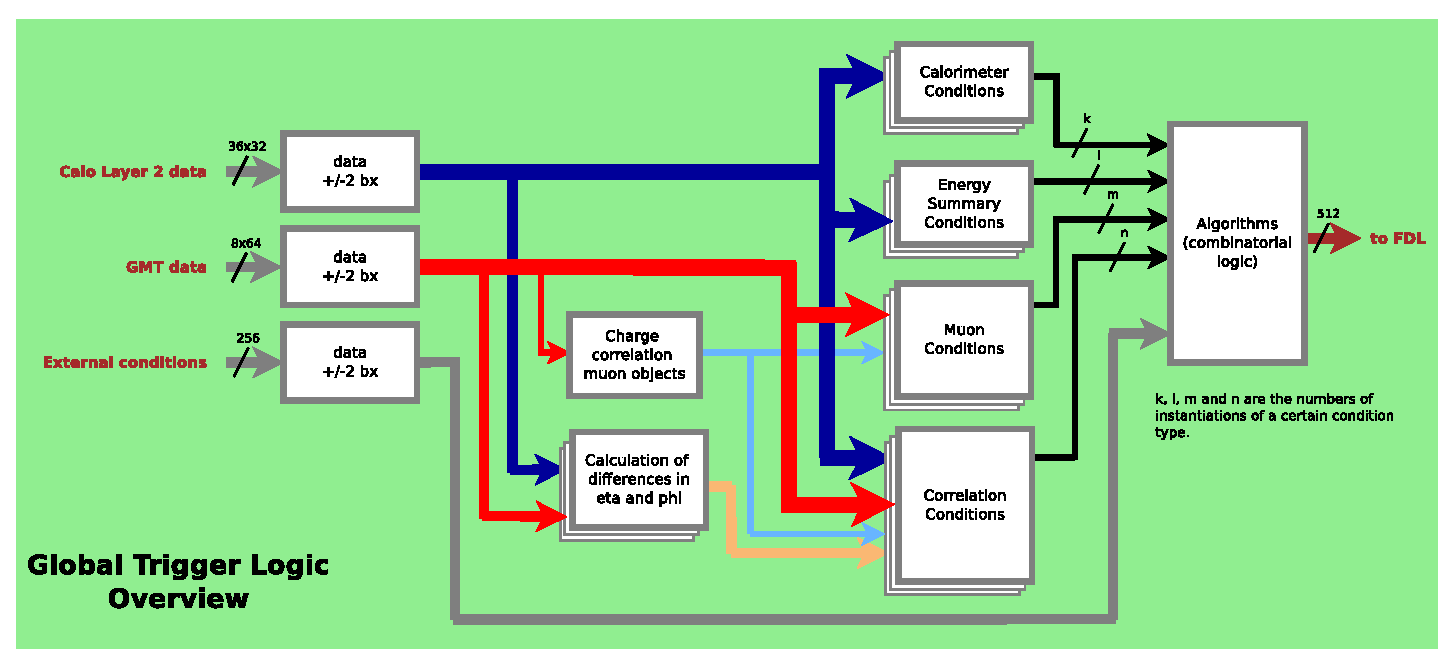
\includegraphics[width=15cm]{figures/mGTL_firmware}
\caption{\ugtl firmware} 
\label{fig:gtl:mGTL_firmware}
\end{figure}

\subsection{\ugtl Interface}
\label{sec:gtl:ugtl_interface}

\textbf{Inputs:}
\begin{itemize}
\item Calo-Layer2 data
\begin{itemize}
\item Electron/$\gamma$ objects
\item Jet objects
\item Tau objects
\item Energy summary information: Total Et (\ett), total Et from ECAL only (ETTEM), total calibrated Et in jets (\htt), missing Et (\etm), missing Et including HF (ET$_{miss}^{HF}$), missing Ht objects (\htm),
missing Ht including HF (HT$_{miss}^{HF}$) and "Asymmetry" information (ASYMET, ASYMHT, ASYMETHF, ASYMHTHF) 
\item Minimum bias HF bits (included in energy summary information data structure)
\item Towercount bits (number of firing HCAL towers, included in energy summary information data structure)
\item "Centrality" bits
\end{itemize}
\item \gmt data
\item External conditions
\item LHC-clock 
\end{itemize}
\textbf{Outputs:}
\begin{itemize}
\item Algorithms
\end{itemize}

\subsection{Definition of optical interfaces}
\label{sec:gtl:optical_interfaces}

Remark: all definitions in the following chapters are from a CMS Detector Note: "Scales for inputs to $\mu$GT" (see actual version in \url{http://globaltrigger.hephy.at/upgrade/ugt/downloads/}).

\subsubsection{Calo-Layer2 optical interfaces}
\label{sec:gtl:gct_optical_interfaces}

The data structure of an \egamma object (bits 27..31 are not defined yet, reserved for quality, ...):
\begin{center}
\begin{bytefield}[boxformatting={\centering\itshape}, bitwidth=1.2em, endianness=big]{32}
        \bitheader{0,8,9,16,17,24,25,26,27,31} \\
        \bitbox {5}     {\texttt{qual/spare}} &
        \bitbox {2}     {\texttt{iso}} &
        \bitbox {8}     {\texttt{$\varphi$}}  &
        \bitbox {8}     {\texttt{$\eta$}}  &
        \bitbox {9}     {\texttt{\et}} \\
\end{bytefield}
\end{center}

The data structure of a jet object (bits 27..31 are not defined yet, reserved for quality, ...):
\begin{center}
\begin{bytefield}[boxformatting={\centering\itshape}, bitwidth=1.2em, endianness=big]{32}
        \bitheader{0,10,11,18,19,26,27,31} \\
        \bitbox {5}     {\texttt{iso/qu/sp}} &
        \bitbox {8}     {\texttt{$\varphi$}}  &
        \bitbox {8}     {\texttt{$\eta$}}  &
        \bitbox {11}    {\texttt{\et}} \\
\end{bytefield}
\end{center}

The data structure of a tau object (bits 27..31 are not defined yet, reserved for quality, ...):
\begin{center}
\begin{bytefield}[boxformatting={\centering\itshape}, bitwidth=1.2em, endianness=big]{32}
        \bitheader{0,8,9,16,17,24,25,26,27,31} \\
        \bitbox {5}     {\texttt{qual/spare}} &
        \bitbox {2}     {\texttt{iso}} &
        \bitbox {8}     {\texttt{$\varphi$}}  &
        \bitbox {8}     {\texttt{$\eta$}}  &
        \bitbox {9}     {\texttt{\et}} \\
\end{bytefield}
\end{center}

The data structure of "total Et" (\ett) quantity [including "total Et from ECAL only" (ETTEM) and "minimum bias HF+ threshold 0" bits]:
\begin{center}
\begin{bytefield}[boxformatting={\centering\itshape}, bitwidth=1.2em, endianness=big]{32}
        \bitheader{0,11,12,23,24,27,28,31} \\
        \bitbox {4}    {\texttt{MBT0HFP}} &
        \bitbox {4}    {\texttt{spare}} &
        \bitbox {12}    {\texttt{\et [ETTEM]}} &
        \bitbox {12}    {\texttt{\et [\ett]}} \\
\end{bytefield}
\end{center}

The data structure of "total calibrated Et in jets" (\htt) quantity [including "towercount" and "minimum bias HF- threshold 0" bits]:
\begin{center}
\begin{bytefield}[boxformatting={\centering\itshape}, bitwidth=1.2em, endianness=big]{32}
        \bitheader{0,11,12,24,25,27,28,31} \\
        \bitbox {4}    {\texttt{MBT0HFM}} &
        \bitbox {3}    {\texttt{spare}} &
        \bitbox {13}    {\texttt{TOWERCOUNT}} &
        \bitbox {12}    {\texttt{\et}} \\
\end{bytefield}
\end{center}

The data structure of "missing Et" (\etm) quantity [including "Asymmetry" ASYMET and "minimum bias HF+ threshold 1" bits]:
\begin{center}
\begin{bytefield}[boxformatting={\centering\itshape}, bitwidth=1.2em, endianness=big]{32}
        \bitheader{0,11,12,19,20,27,28,31} \\
        \bitbox {4}    {\texttt{MBT1HFP}} &
        \bitbox {8}    {\texttt{ASYMET}} &
        \bitbox {8}     {\texttt{$\varphi$}} &
        \bitbox {12}    {\texttt{\et}} \\
\end{bytefield}
\end{center}

The data structure of "missing Ht" (\htm) quantity [including "Asymmetry" ASYMHT and "minimum bias HF- threshold 1" bits]:
\begin{center}
\begin{bytefield}[boxformatting={\centering\itshape}, bitwidth=1.2em, endianness=big]{32}
        \bitheader{0,11,12,19,20,27,28,31} \\
        \bitbox {4}    {\texttt{MBT1HFM}} &
        \bitbox {8}    {\texttt{ASYMHT}} &
        \bitbox {8}     {\texttt{$\varphi$}} &
        \bitbox {12}    {\texttt{\et}} \\
\end{bytefield}
\end{center}

The data structure of "missing Et including HF" (ET$_{miss}^{HF}$) quantity [including "Asymmetry" ASYMETHF and "Centrality" bits (3:0)]:
\begin{center}
\begin{bytefield}[boxformatting={\centering\itshape}, bitwidth=1.2em, endianness=big]{32}
        \bitheader{0,11,12,19,20,27,28,31} \\
        \bitbox {4}    {\small  \texttt{[CENT3:0]}} &
        \bitbox {8}    {\texttt{ASYMETHF}} &
        \bitbox {8}     {\texttt{$\varphi$}} &
        \bitbox {12}    {\texttt{\et}} \\
\end{bytefield}
\end{center}

The data structure of "missing Ht including HF" (HT$_{miss}^{HF}$) quantity [including "Asymmetry" ASYMHTHF and "Centrality" bits (7:4)]:
\begin{center}
\begin{bytefield}[boxformatting={\centering\itshape}, bitwidth=1.2em, endianness=big]{32}
        \bitheader{0,11,12,19,20,27,28,31} \\
        \bitbox {4}    {\small  \texttt{CENT[7:4]}} &
        \bitbox {8}    {\texttt{ASYMHTHF}} &
        \bitbox {8}     {\texttt{$\varphi$}} &
        \bitbox {12}    {\texttt{\et}} \\
\end{bytefield}
\end{center}

\subsubsection{\gmt optical interfaces}
\label{sec:gtl:gmt_optical_interfaces}

The data structure of a muon object (64 bits - bit 34 = charge sign, bit 35 = charge valid, bit 61 is a spare bit, bit 63..62 = impact parameter):
\begin{center}
\begin{bytefield}[boxformatting={\centering\itshape}, endianness=big, bitwidth=1.2em]{32}
        \bitheader[lsb=32]{32,33,34,35,36,42,43,52,53,60,61,61,62,63} \\
        \bitbox {2}     {\small  \texttt{imp para}}       &
        \bitbox {1}     {\small  \texttt{r}}       &
        \bitbox {8}     {\texttt{unconst.\pt}}       &
        \bitbox {10}    {\texttt{$\varphi$} (out)}
        \bitbox {7}     {\texttt{index bits}}
        \bitbox {2}     {\small  \texttt{ch}}       &
        \bitbox {2}     {\small \texttt{iso}} \\
        [3ex]
        \bitheader{0,9,10,18,19,22,23,31} \\
        \bitbox {9}     {\texttt{$\eta$} (extrapol.)}       &
        \bitbox {4}     {\texttt{qual}}       &
        \bitbox {9}     {\texttt{\pt}}    &
        \bitbox {10}    {\texttt{$\varphi$} (extrapol.)} \\
\end{bytefield}
\end{center}

\clearpage

\subsection{Implementation in firmware}
\label{sec:gtl:implementation_firmware_gtl}

Remark: all definitions for scales in the following chapters are from a CMS Detector Note: "Scales for inputs to $\mu$GT" (see actual version in \url{http://globaltrigger.hephy.at/upgrade/ugt/downloads/}).

The firmware of \ugtl consists of two main parts:
\begin{itemize}
\item A top-of-hierarchy file (\texttt{gtl\_module.vhd}), which contains the pipeline for $\pm$2bx data, the instantiations of calculators for differences in $\eta$ and $\varphi$, the instantiations of
conditions, the instantiations of charge correlation logic of muons and the Algorithms logic for 512 Algorithms, as well as a package file (\texttt{gtl\_pkg.vhd}) for declarations.
Both files generated by VHDL Producer for every Trigger Menu (see Figure~\ref{fig:gtl:tme_gtl}). In addition, VHDL Producer creates a VHDL files
for the mapping of Algorithms (\texttt{algo\_mapping\_rop.vhd}) for \ufdl.
\item A set of VHDL-files for all the modules instantiated in top-of-hierarchy and the modules in the hierarchy. These files, called the "fixed part", are not influenced by VHDL Producer. 
\end{itemize}

\begin{figure}[htb]
\centering
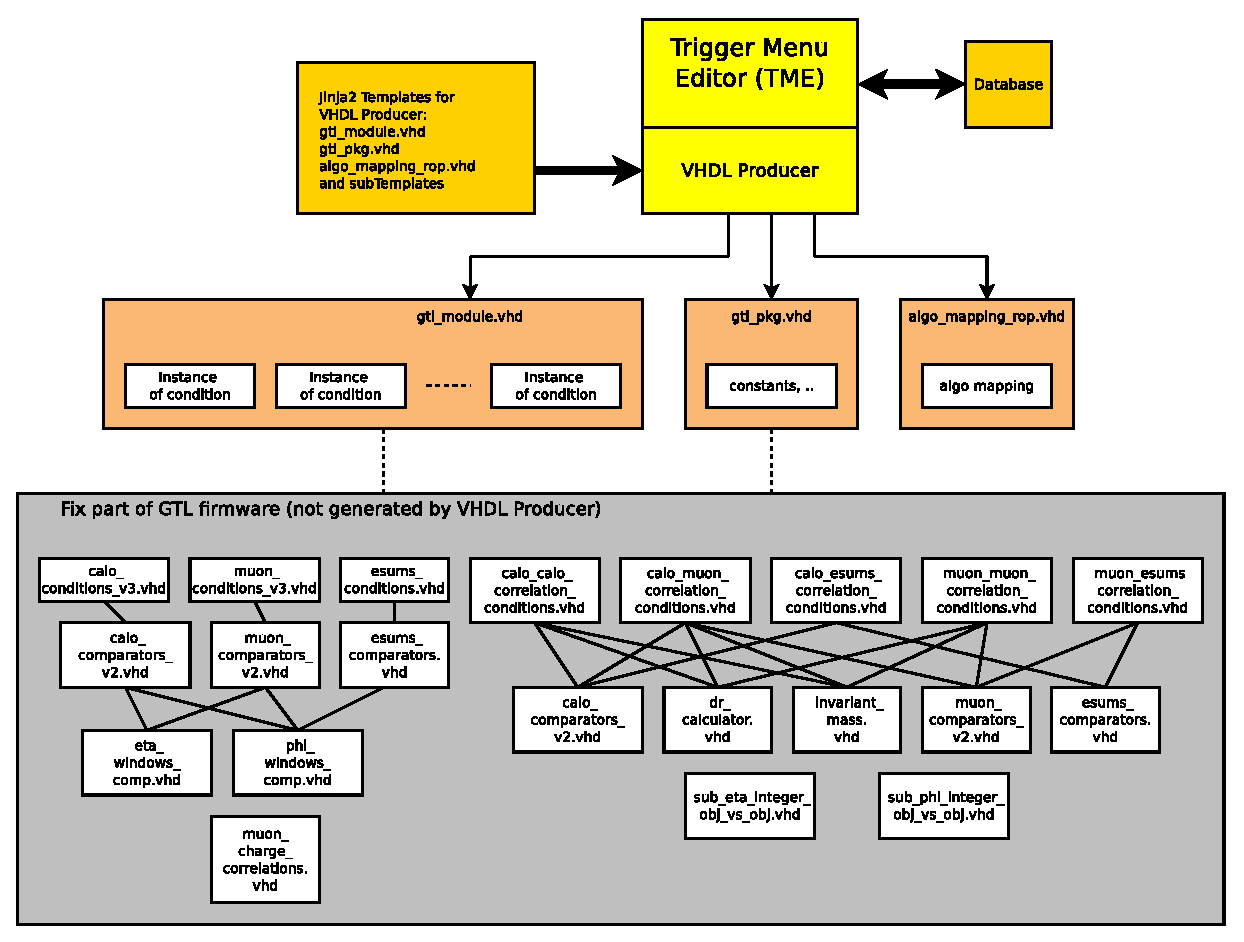
\includegraphics[width=15cm]{figures/tme_gtl}
\caption{VHDL file generation by VHDL Producer} 
\label{fig:gtl:tme_gtl}
\end{figure}

The latency of \ugtl is fixed to 5 bunch crossings,
2 bunch crossings for the pipeline of $\pm$2bx data (for data with +2bx and +1bx), 2 bunch crossings for conditions (fixed), also for the conditions requested in the future,
1 bunch crossing for the logic of Algorithms (See Figure \ref{fig:gtl:gtl_pipeline}).\\

If there are not enough firmware resources in FPGA of one AMC board for 512 Algorithms, more boards could be used. Therefore the 512 Algorithms are \textbf{partitioned by TME} (\eg the first board covers
Algorithms 0..200 and the second Algorithms 201..511). Trigger Menu Editor (TME) will give the number of Algorithms per module as constant in the package module \texttt{gtl\_pkg.vhd}.
This means \ugtl and \ufdl firmware considered as a unit for synthesis.\\

\subsubsection{Top-of-hierarchy module}
\label{sec:gtl:top_module}

The top-of-hierarchy module (\texttt{gtl\_module.vhd}) contains 
\begin {itemize}
\item the pipeline for $\pm$2bx data
\item the instantiations of charge correlation logic of muons (generated by VHDL Producer)
\item the instantiations of calculators for differences in $\eta$ and $\varphi$ (generated by VHDL Producer)
\item the instantiations of conditions (generated by VHDL Producer)
\item a boolean logic for Algorithms (generated by VHDL Producer)
\end {itemize}

\subsubsection{Package module}
\label{sec:gtl:package_module}

All the declarations for arrays ('type'), parameters ('constant') and look-up-tables ('constant') used in modules are in \texttt{gtl\_pkg.vhd} package-file.

\clearpage

\subsection{\ugtl structure}
\label{sec:gtl:mgtl_structure}

\subsubsection{Data $\pm$2bx}
\label{sec:gtl:data_p_m_2bx}

The \ugtl input data flow through a register pipeline of four stages. With those data it is possible to have conditions with objects from
different bunch crossings (within $\pm$2 bunch crossings), \eg for Correlation conditions.\\
See Figure \ref{fig:gtl:gtl_pipeline} for a scheme of \ugtl pipeline structure. The data "data\_p\_1bx" and "data\_p\_2bx" occur 1 respectively 2 bunch crossings
after data for a certain bunch crossing, therefore we got 2 bunch crossings of latency from those data. The data "data\_m\_1bx" and "data\_m\_2bx" have no influence
on latency, because coming before data for a certain bunch crossing.

\begin{figure}[htb]
\centering
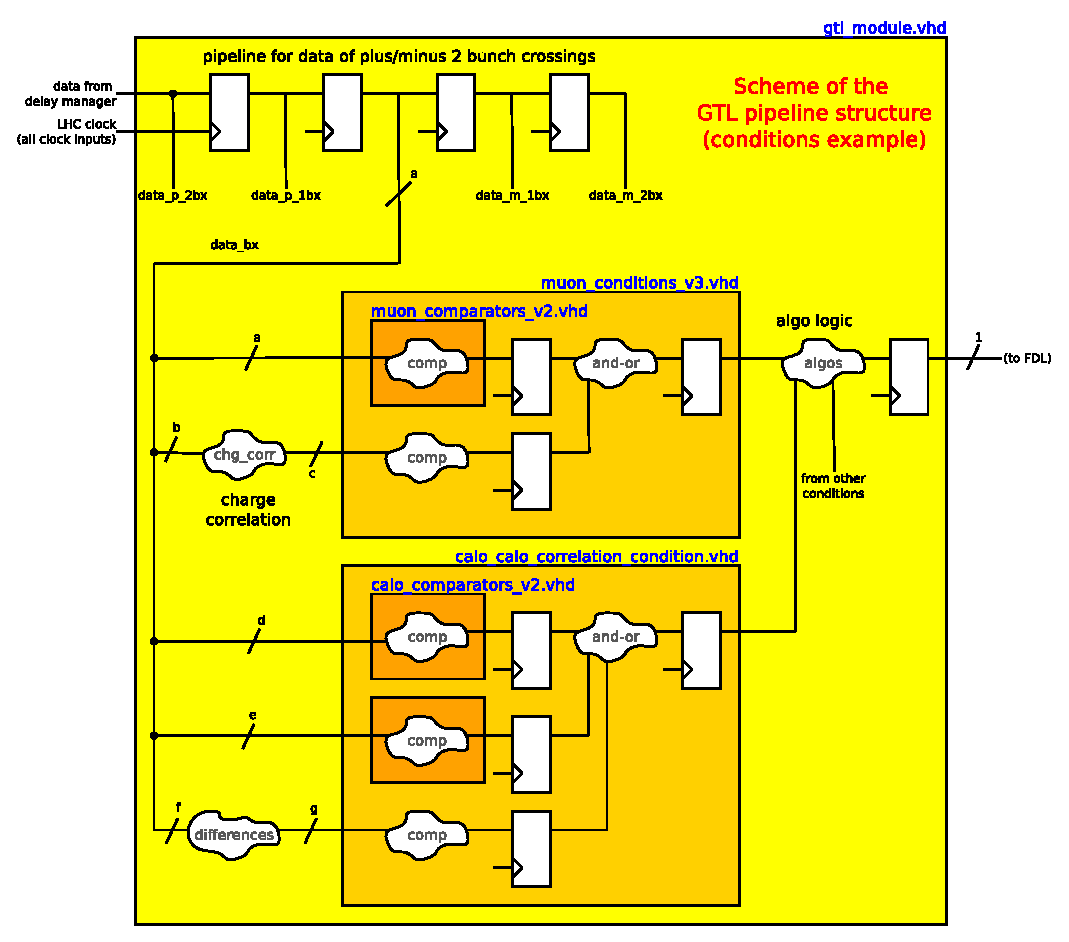
\includegraphics[width=15cm]{figures/gtl_pipeline}
\caption{Scheme of \ugtl pipeline structure} 
\label{fig:gtl:gtl_pipeline}
\end{figure}

\subsubsection{Calculation of differences in $\eta$ and $\varphi$}
\label{sec:gtl:calculation_differences}

Some condition types namely correlation conditions uses differences in $\eta$ and $\varphi$ to make the decision.
Therefore these differences are calculated out of these conditions, because the differences can be used several times in different condition types.
The differences in $\eta$ and $\varphi$ are calculated in bins. These differences in bins are converted to numbers (by LUTs),
which represents values of differences (multiples of units in $\eta$ and $\varphi$).
Differences in $\varphi$ are provided by module \texttt{sub\_phi\_integer\_obj\_vs\_obj.vhd}, which instantiates the module \texttt{sub\_unsigned\_phi.vhd} as many times as
the numbers of both objects determine.\\
In the module \texttt{sub\_unsigned\_phi.vhd} a calculation of a difference of two objects is done, both objects must have the same resolution, namely the higher one.
The result is the absolute value of the difference.
There are two differences in $\varphi$, one "clockwise" and one "anti-clockwise". For the final result the smaller difference is taken.\\
Differences in $\eta$ are provided by module \texttt{sub\_eta\_integer\_obj\_vs\_obj.vhd}, which instantiates the module \texttt{sub\_signed\_eta.vhd} as many times as
the numbers of both objects determine.\\
In the module \texttt{sub\_signed\_eta.vhd} a calculation of a difference of two objects is done with a signed subtraction, because of the Two's Complement notation of $\eta$ values.
The result is the absolute value of the difference. 

\subsubsection{Calorimeter conditions}
\label{sec:gtl:calorimeter_conditions}

\paragraph{Calorimeter data}
\label{sec:gtl:calorimeter_data}

The calorimeter trigger processing identifies \textbf{\egamma, jet and tau} objects and \textbf{\esums}.\\

\textbf{\egamma}:\\ Twelve objects are passed to the \ugt for each event.\\
For each selected object, the Calo-Layer2 sends parameters for \et and for position and quality information - encoded in 32 bits: 
\begin{itemize}
\item 9 bits \et, range = 0..255 GeV (HW index = 0..0x1FF), step = 0.5, the highest bin will mark an overflow (HW index 0x1FF): meaning has to be defined
\item 8 (7+1 sign) bits pseudo-rapidity ($\eta$) position, range = -3.0 to 3.0, step = 0.087/2, linear scale, 138 bins (HW index = 0xBC..0x44)
\item 8 bits azimuth angle ($\varphi$) position, range = 2$\pi$, step $\approx$ 2$\pi$/144 (\^=2.5°), 144 bins (HW index = 0..0x8F), HW index starting at 0° (anti-clockwise)
\item 2 bits isolation (meaning not defined yet!) 
\item 5 bits quality and spare (not defined yet!)
\end{itemize}

The data structure of an \egamma object (bits 27..31 are not defined yet, reserved for quality, ...):
\begin{center}
\begin{bytefield}[boxformatting={\centering\itshape}, bitwidth=1.2em, endianness=big]{32}
        \bitheader{0,8,9,16,17,24,25,26,27,31} \\
        \bitbox {5}     {\texttt{qual/spare}} &
        \bitbox {2}     {\texttt{iso}} &
        \bitbox {8}     {\texttt{$\varphi$}}  &
        \bitbox {8}     {\texttt{$\eta$}}  &
        \bitbox {9}     {\texttt{\et}} \\
\end{bytefield}
\end{center}

\textbf{jet}:\\ Twelve objects are passed to the \ugt for each event.\\
For each selected object, the Calo-Layer2 sends parameters: \et, for position and quality information - encoded in 32 bits: 
\begin{itemize}
\item 11 bits \et, range = 0..1023 GeV (HW index = 0..0x7FF), step = 0.5, the highest bin will mark an overflow (HW index 0x7FF): meaning has to be defined
\item 8 (7+1 sign) bits pseudo-rapidity ($\eta$) position, range = -5.0 to 5.0, step = 0.087/2, linear scale, 230 bins (HW index = 0x8E..0x72)
\item 8 bits azimuth angle ($\varphi$) position, range = 2$\pi$, step $\approx$ 2$\pi$/144 (\^=2.5°), 144 bins (HW index = 0..0x8F), HW index starting at 0° (anti-clockwise)
\item 5 bits quality and spare (not defined yet!)
\end{itemize}

The data structure of a jet object (bits 27..31 are not defined yet, reserved for quality, ...):
\begin{center}
\begin{bytefield}[boxformatting={\centering\itshape}, bitwidth=1.2em, endianness=big]{32}
        \bitheader{0,10,11,18,19,26,27,31} \\
        \bitbox {5}     {\texttt{iso/qu/sp}} &
        \bitbox {8}     {\texttt{$\varphi$}}  &
        \bitbox {8}     {\texttt{$\eta$}}  &
        \bitbox {11}    {\texttt{\et}} \\
\end{bytefield}
\end{center}

\textbf{tau}:\\ Twelve objects are passed to the \ugt for each event.\\
For each selected object, the Calo-Layer2 sends parameters for \et and for position and quality information - encoded in 32 bits: 
\begin{itemize}
\item 9 bits \et, range = 0..255 GeV (HW index = 0..0x1FF), step = 0.5, the highest bin will mark an overflow (HW index 0x1FF): meaning has to be defined
\item 8 (7+1 sign) bits pseudo-rapidity ($\eta$) position, range = -3.0 to 3.0, step = 0.087/2, linear scale, 138 bins (HW index = 0xBC..0x44)
\item 8 bits azimuth angle ($\varphi$) position, range = 2$\pi$, step $\approx$ 2$\pi$/144 (\^=2.5°), 144 bins (HW index = 0..0x8F), HW index starting at 0° (anti-clockwise)
\item 2 bits isolation (meaning not defined yet!) 
\item 5 bits quality and spare (not defined yet!)
\end{itemize}

The data structure of a tau object (bits 27..31 are not defined yet, reserved for quality, ...):
\begin{center}
\begin{bytefield}[boxformatting={\centering\itshape}, bitwidth=1.2em, endianness=big]{32}
        \bitheader{0,8,9,16,17,24,25,26,27,31} \\
        \bitbox {5}     {\texttt{qual/spare}} &
        \bitbox {2}     {\texttt{iso}} &
        \bitbox {8}     {\texttt{$\varphi$}}  &
        \bitbox {8}     {\texttt{$\eta$}}  &
        \bitbox {9}     {\texttt{\et}} \\
\end{bytefield}
\end{center}

The representation of the 8 bits (called "hardware index [HW index]") in $\eta$ is expected as Two's Complement notation as shown in Table~\ref{tab:gtl:calo_eta_scale}.\\
 
\begin{table}[htdp]
\caption{$\eta$ scale of \egamma and tau}
\begin{center}
\begin{tabular}{|c|l|c|}\hline
\textbf{HW index}& \textbf{$\eta$ range} & \textbf{$\eta$ bin}\\\hline\hline
0x44 & 68$*$0.087/2 to 69$*$0.087/2 & 68\\\hline
... & ... & ...\\\hline
0x01 & 0.087/2 to 2$*$0.087/2 & 1\\\hline
0x00 & 0 to 0.087/2 & 0\\\hline
0xFF & 0 to -0.087/2 & -1\\\hline
0xFE & -0.087/2 to -2$*$0.087/2 & -2\\\hline
... & ... & ...\\\hline
0xBC & -68$*$0.087/2 to -69$*$0.087/2 & -69\\\hline
\end{tabular}
\end{center}
\label{tab:gtl:calo_eta_scale}
\end{table}

\begin{table}[htdp]
\caption{$\eta$ scale of jet}
\begin{center}
\begin{tabular}{|c|l|c|}\hline
\textbf{HW index}& \textbf{$\eta$ range} & \textbf{$\eta$ bin}\\\hline\hline
0x72 & 114$*$0.087/2 to 115$*$0.087/2 & 114\\\hline
... & ... & ...\\\hline
0x01 & 0.087/2 to 2$*$0.087/2 & 1\\\hline
0x00 & 0 to 0.087/2 & 0\\\hline
0xFF & 0 to -0.087/2 & -1\\\hline
0xFE & -0.087/2 to -2$*$0.087/2 & -2\\\hline
... & ... & ...\\\hline
0x8E & -114$*$0.087/2 to -115$*$0.087/2 & -115\\\hline
\end{tabular}
\end{center}
\label{tab:gtl:calo_eta_scale}
\end{table}

The representation of the 8 bits in $\varphi$ is expected as shown in Table~\ref{tab:gtl:calo_phi_scale}.\\
 
\begin{table}[htdp]
\begin{center}
\begin{tabular}{|c|l|l|c|}\hline
HW index & $\varphi$ range & $\varphi$ range [degrees] & $\varphi$ bin\\\hline\hline
0x00 & 0 to 2$\pi$/144 & 0 to 2.5 & 0\\\hline
0x01 & 2$\pi$/144 to 2$*$2$\pi$/144 & 2.5 to 5.0 & 1\\\hline
... & ... & ... & ...\\\hline
0x8F & 143$*$2$\pi$/144 to 2$\pi$ & 357.5 to 360 & 143\\\hline
\end{tabular}
\end{center}
\caption{$\varphi$ scale of calorimeter objects}
\label{tab:gtl:calo_phi_scale}
\end{table}

The representation of the 2 bits for isolation (e/$\gamma$ and tau) is expected as shown in Table~\ref{tab:gtl:eg_tau_iso_bits}.\\

\begin{table}[ht]
\caption{Definition of e/$\gamma$ and tau isolation bits}
\vspace{5mm}
\centering
\begin{tabular}{|c|c|}\hline
bits [26..25] & definition \\\hline\hline
00 & not isolated \\
01 & isolated \\
10 & TBD \\
11 & TBD \\\hline
\end{tabular}
\label{tab:gtl:eg_tau_iso_bits}
\end{table}

\clearpage

\paragraph{Calorimeter conditions definition}\label{sec:gtl:calo_cond_def}

A condition consists of calorimeter objects as input data and a set of requirements, which contain the requirements to be complied.

The requirement for calorimeter conditions contains:\\
one threshold for \et, ranges for $\eta$, $\varphi$ LUTs for isolation and differences in $\eta$ and $\varphi$. In addition the selection of the "relative bx" of objects
is done in the requirement.\\
The condition is complied, if every comparison between object parameters and requirements is valid for the following equation:
\begin{itemize}
\item \et greater-equal or equal threshold
\item $\eta$ in range
\item $\varphi$ in range
\item isolation as requested (for \egamma and tau)
\end{itemize}
\textit{Additional comparisons for "quality information" could be part of the equation - but not defined yet.}

There are different types of calorimeter conditions implemented, depending of how many objects have to comply the requirements.
\begin{itemize}
\item "Quad objects requirements condition": this condition type consists of requirements for 4 different trigger objects of the same object type. 
For each object the requirements can be different. To fulfill this condition, there must exist at least one set of 4 different objects,
each of which fulfills at least one of the requirements.
\item "Triple objects requirements condition": this condition type consists of requirements for 3 different trigger objects of the same object type. 
For each object the requirements can be different. To fulfill this condition, there must exist at least one set of 3 different objects,
each of which fulfills at least one of the requirements.
\item "Double objects requirements condition": this condition type consists of requirements for 2 different trigger objects of the same object type. 
For each object the requirements can be different. To fulfill this condition, there must exist at least one set of 2 different objects,
each of which fulfills at least one of the requirements.\footnote{"Double objects requirements condition with spatial correlation" not used anymore, replaced by Correlation conditions}
\item "Single object requirement condition": this condition type consists of one requirement for one trigger object of a given object type. 
To fulfill this condition, there must exist at least one object which fulfills the requirement.

\end{itemize}

The selection of the mode of \et-comparator (greater/equal or equal), the \et-threshold-value, ranges for $\eta$ and $\varphi$ set with thresholds, LUTs for isolation and ranges for differences in $\eta$ and $\varphi$ set with thresholds are fixed values given by VHDL Producer for every Trigger Menu.
The objects have to be of same type and same bunch-crossing.

\subparagraph{Calorimeter conditions module}\label{sec:gtl:calo_conditions_module}

The module for conditions with calorimeter objects (\texttt{calo\_conditions.vhd}) instantiates the calorimeter comparators module (\texttt{calo\_comparators.vhd}) as many times as the numbers of objects and requirements determine. 

For comparison in $\eta$, $\varphi$ and the differences in $\eta$ and $\varphi$, "window"-comparators are used.\\
In the calorimeter conditions module a cut for two-body pt calculation can be selected (see ~\ref{sec:gtl:twobody_pt_calculation}). Therefore a threshold value for two-body pt is required.\\

\subparagraph{Calorimeter Overlap Remover conditions module}\label{sec:gtl:calo_conditions_orm_module}
The Calorimeter Overlap Remover conditions consits of a Calorimeter condition (\ref{sec:gtl:calo_conditions_module}) and a single condition for a different calo object type. One or more correlation cut(s) ($\Delta\eta$, $\Delta\varphi$ and $\Delta$$R$ - \ref{sec:gtl:correlation_conditions}) for overlap removal is required between different calo object types.
Overlap Remover conditions \texttt{calo\_conditions\_orm.vhd} are implemented only for calo object types.

\subparagraph{Calorimeter comparators module}\label{sec:gtl:calo_comp_module}
A comparator between the energy (\et) and a threshold (et\_threshold) and a comparison in $\eta$ with five "window"-comparators and $\varphi$ with two "window"-comparators
is done in this basic module. The values for \et threshold, the 'mode-selection' for the \et comparator and the "limits" of the "window"-comparators 
is given in the generic interface list of the module. Additionally the data-structure of input data (data\_i in port interface list) is provided
as a record in this list. The output signal of the module is in high state, if all comparisons are true.\\
The comparison in $\eta$ is done with five "window"-comparators, so one gets max. five ranges for $\eta$. The $\eta$ value (HW index) has a Two's Complement notation, the comparisons is done signed. Number of windows is given for $\eta$.\\
The comparison in $\varphi$ is done with two "window"-comparators, so one gets two ranges for $\varphi$. The comparisons is done unsigned. There are two flags, one for "full-range" and one for "ignore-second-window" for the selection of the ranges.\\
There are two cases how the limits of one "window"-comparator could be set (see also Figure~\ref{fig:gtl:phi_windows_comparator} and Listing~\ref{lst:phi_window_comparator_vhd}):
\begin{itemize}
\item Upper limit is less than lower limit => $\varphi$ range between the limits, including the $\varphi$ bin with value = 0 (HW index).
\item Upper limit is greater/equal than lower limit => $\varphi$ range between the limits, not including the $\varphi$ bin with value = 0 (HW index).
\end{itemize}
The comparison of isolation (for \egamma and tau) is done with LUTs.
\begin{lstlisting}[label=lst:phi_window_comparator_vhd,float=here,caption=VHDL code of "window"-comparator in $\varphi$,captionpos=t]
    phi_comp_w1 <= '1' when phi_w1_upper_limit < phi_w1_lower_limit and
                    (phi <= phi_w1_upper_limit or phi >= phi_w1_lower_limit) else
                   '1' when phi_w1_upper_limit >= phi_w1_lower_limit and
                    (phi <= phi_w1_upper_limit and phi >= phi_w1_lower_limit)
                    else '0';
\end{lstlisting}

The values of $\eta$ and $\varphi$ have to be inside of only one of the required ranges ("or").

The comparison of isolation (for \egamma and tau) is done with LUTs (see Table~\ref{tab:gtl:calo_lut_iso}).
Only the least significant 4 bits of LUT are used, because currently 2 isolation bits are defined. 

\begin{table}[htdp]
\begin{center}
\begin{tabular}{|c|c|p{.4\columnwidth}|}\hline
LUT content (16 bits) & isolation bits [26..25] & trigger \\\hline\hline
X"0" & xx & no trigger\\\hline
X"1" & 00 & trigger on isolation bits = 00\\\hline
X"2" & 01 & trigger on isolation bits = 01\\\hline
X"3" & 00 or 01 & trigger on isolation bits = 00 or 01\\\hline
X"4" & 10 & trigger on isolation bits = 10\\\hline
X"5" & 00 or 10 & trigger on isolation bits = 00 or 10\\\hline
X"6" & 01 or 10 & trigger on isolation bits = 01 or 10\\\hline
X"7" & 00 or 01 or 10 & trigger on isolation bits = 00 or 01 or 10\\\hline
X"8" & 11 & trigger on isolation bits = 11\\\hline
X"9" & 00 or 11 & trigger on isolation bits = 00 or 11\\\hline
X"A" & 01 or 11 & trigger on isolation bits = 01 or 11\\\hline
X"B" & 00 or 01 or 11 & trigger on isolation bits = 00 or 01 or 11\\\hline
X"C" & 10 or 11 & trigger on isolation bits = 10 or 11\\\hline
X"D" & 00 or 10 or 11 & trigger on isolation bits = 00 or 10 or 11\\\hline
X"E" & 01 or 10 or 11 & trigger on isolation bits = 01 or 10 or 11\\\hline
X"F" & 00 or 01 or 10 or 11 & trigger on isolation bits = 00 or 01 or 10 or 11 (= "ignore" isolation)\\\hline
\end{tabular}
\end{center}
\caption{LUT contents for isolation comparison of \egamma and tau objects}
\label{tab:gtl:calo_lut_iso}
\end{table}

\begin{figure}[htb]
\centering
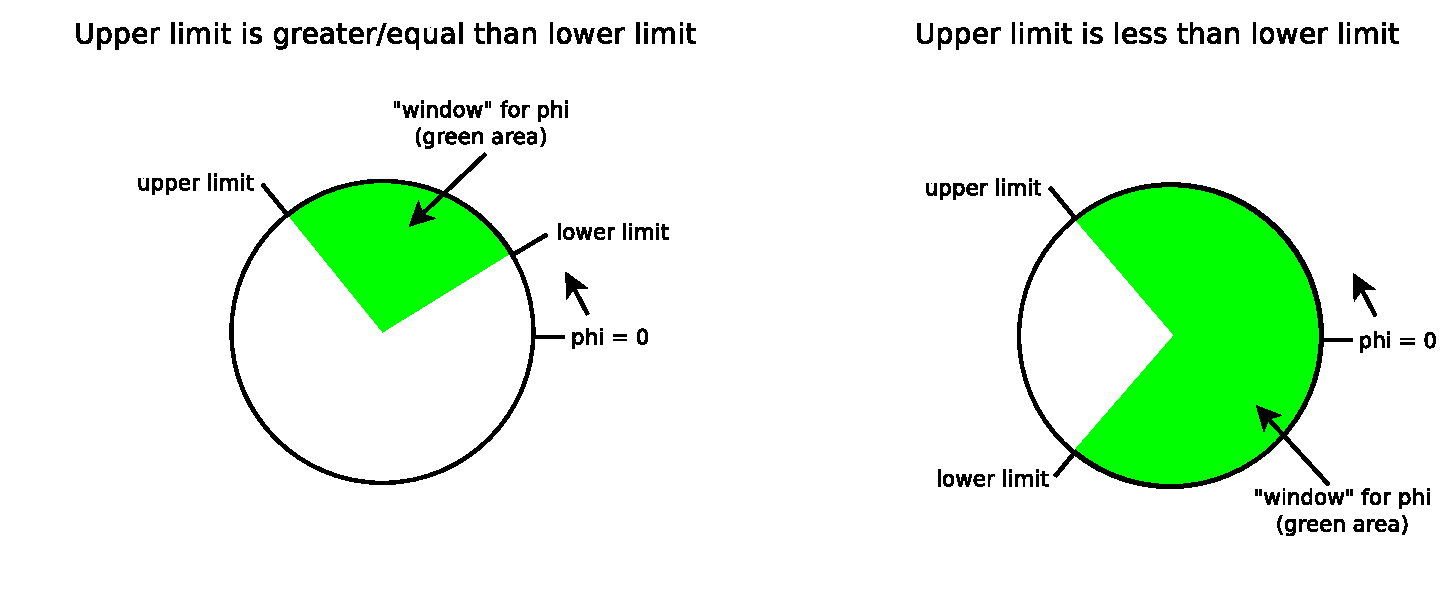
\includegraphics[width=15cm]{figures/phi_windows_comparator}
\caption{Setting the limits for "window"-comparators for $\varphi$} 
\label{fig:gtl:phi_windows_comparator}
\end{figure}

\clearpage

\subsubsection{Energy sum quantities conditions}
\label{sec:gtl:esums_conditions}

\textbf{\esums}:\\ Consists of following quantities (naming convention see \ref{sec:glossary}):
\begin{itemize}
\item \textbf{\ett}
\item \textbf{\htt}
\item \textbf{\etm}
\item \textbf{\htm}
\item \textbf{ETTEM}
\item \textbf{ET$_{miss}^{HF}$}
\item \textbf{HT$_{miss}^{HF}$}
\item \textbf{ASYMET}
\item \textbf{ASYMHT}
\item \textbf{ASYMETHF}
\item \textbf{ASYMHTHF}
\item \textbf{CENT0}
\item \textbf..
\item \textbf{CENT7}
\end{itemize}

\paragraph{Energy sum quantities data}
Calo-Layer2 sends 6 frames (each 32 bits) with Energy sum quantities containing the following information:
\begin{itemize}
\item \et, 12 bits, range = 0..2047 GeV (HW index = 0..0xFFF), step = 0.5, the highest bin will mark an overflow (HW index 0xFFF): meaning has to be defined
\item azimuth angle ($\varphi$) position, 8 bits, range = 2$\pi$, step $\approx$ 2$\pi$/144 (\^=2.5°), 144 bins (HW index = 0..0x8F), HW index starting at 0° (anti-clockwise)
\item "Towercount", 13 bits, range = 0..8191
\item "Minimum bias", 4 bits, range = 0..15
\item "Asymmetry", 8 bits, range = 0..255 (used 0..100)
\item "Centrality", 8 bits, used as signals
\end{itemize}

Frame0: The data structure of "total Et" (\ett) quantity [including "total Et from ECAL only" (ETTEM) and "minimum bias HF+ threshold 0" bits]:
\begin{center}
\begin{bytefield}[boxformatting={\centering\itshape}, bitwidth=1.2em, endianness=big]{32}
        \bitheader{0,11,12,23,24,27,28,31} \\
        \bitbox {4}    {\texttt{MBT0HFP}} &
        \bitbox {4}    {\texttt{spare}} &
        \bitbox {12}    {\texttt{\et [ETTEM]}} &
        \bitbox {12}    {\texttt{\et [\ett]}} \\
\end{bytefield}
\end{center}

Frame1: The data structure of "total calibrated Et in jets" (\htt) quantity [including "towercount" and "minimum bias HF- threshold 0" bits]:
\begin{center}
\begin{bytefield}[boxformatting={\centering\itshape}, bitwidth=1.2em, endianness=big]{32}
        \bitheader{0,11,12,24,25,27,28,31} \\
        \bitbox {4}    {\texttt{MBT0HFM}} &
        \bitbox {3}    {\texttt{spare}} &
        \bitbox {13}    {\texttt{TOWERCOUNT}} &
        \bitbox {12}    {\texttt{\et}} \\
\end{bytefield}
\end{center}

Frame2: The data structure of "missing Et" (\etm) quantity [including "Asymmetry" ASYMET and "minimum bias HF+ threshold 1" bits]:
\begin{center}
\begin{bytefield}[boxformatting={\centering\itshape}, bitwidth=1.2em, endianness=big]{32}
        \bitheader{0,11,12,19,20,27,28,31} \\
        \bitbox {4}    {\texttt{MBT1HFP}} &
        \bitbox {8}    {\texttt{ASYMET}} &
        \bitbox {8}     {\texttt{$\varphi$}} &
        \bitbox {12}    {\texttt{\et}} \\
\end{bytefield}
\end{center}

Frame3: The data structure of "missing Ht" (\htm) quantity [including "Asymmetry" ASYMHT and "minimum bias HF- threshold 1" bits]:
\begin{center}
\begin{bytefield}[boxformatting={\centering\itshape}, bitwidth=1.2em, endianness=big]{32}
        \bitheader{0,11,12,19,20,27,28,31} \\
        \bitbox {4}    {\texttt{MBT1HFM}} &
        \bitbox {8}    {\texttt{ASYMHT}} &
        \bitbox {8}     {\texttt{$\varphi$}} &
        \bitbox {12}    {\texttt{\et}} \\
\end{bytefield}
\end{center}

Frame4: The data structure of "missing Et including HF" (ET$_{miss}^{HF}$) quantity [including "Asymmetry" ASYMETHF and "Centrality" bits (3:0)]:
\begin{center}
\begin{bytefield}[boxformatting={\centering\itshape}, bitwidth=1.2em, endianness=big]{32}
        \bitheader{0,11,12,19,20,27,28,31} \\
        \bitbox {4}    {\small \texttt{CENT[3:0]}} &
        \bitbox {8}    {\texttt{ASYMETHF}} &
        \bitbox {8}     {\texttt{$\varphi$}} &
        \bitbox {12}    {\texttt{\et}} \\
\end{bytefield}
\end{center}

Frame5: The data structure of "missing Ht including HF" (HT$_{miss}^{HF}$) quantity [including "Asymmetry" ASYMHTHF and "Centrality" bits (7:4)]:
\begin{center}
\begin{bytefield}[boxformatting={\centering\itshape}, bitwidth=1.2em, endianness=big]{32}
        \bitheader{0,11,12,19,20,27,28,31} \\
        \bitbox {4}    {\small \texttt{CENT[7:4]}} &
        \bitbox {8}    {\texttt{ASYMHTHF}} &
        \bitbox {8}     {\texttt{$\varphi$}} &
        \bitbox {12}    {\texttt{\et}} \\
\end{bytefield}
\end{center}

\paragraph{Energy sum quantities conditions module (including Asymmetry conditions)}

A comparator between \et and a threshold (et\_threshold) and, depending on object type, a comparison in $\varphi$ with 
two "window"-comparators is done in this module. 
The value for \et threshold, the 'mode-selection' for the \et comparator and the limits for the "window"-comparators are given in the generic interface list of the module.
The selection whether a comparison in $\varphi$ is part of the condition is done with the value of the generic parameter 'obj\_type' 
('ETM\_TYPE', 'ETMHF\_TYPE', 'HTM\_TYPE' and 'HTMHF\_TYPE' force a comparison).
The comparison in $\varphi$ is done in the same way as for calorimeter conditions (see \ref{sec:gtl:calo_comp_module}).
Additionally the data-structure of input data (data\_i in port interface list) is provided
as a record in this list. The output signal of the module is in high state, if all comparisons are true.\\
Data for Asymmetry trigger are received on 4 frames on bits 27..20 (8 bits). For every type a comparision with an 8-bit threshold (greater-equal or equal) is done.
Asymmetry data are interpreted as counts.

\subsubsection{Minimum bias trigger conditions}
\label{sec:gtl:min_bias_conditions}

Data for Minimum bias trigger are received on the 4 MSBs of 4 frames used for Energy sum quantities (see \ref{sec:gtl:esums_conditions}). 

\begin{itemize}
\item MBT0HFP: "minimum bias HF+ threshold 0" bits
\item MBT0HFM: "minimum bias HF- threshold 0" bits
\item MBT1HFP: "minimum bias HF+ threshold 1" bits
\item MBT1HFM: "minimum bias HF- threshold 1" bits
\end{itemize}

In the min\_bias\_hf\_conditions.vhd module there is a comparision with a 4-bit threshold (greater-equal or equal).

\subsubsection{Towercount condition}
\label{sec:gtl:towercount_cond}

Data for Towercount trigger (number of firing HCAL towers) are received on frame \htt (see \ref{sec:gtl:esums_conditions}) on bits 24..12 (13 bits) of \htt data structure. 
In the towercount\_condition.vhd module there is a comparision with a 13-bit threshold (greater-equal or equal).

\subsubsection{Centrality condition}
\label{sec:gtl:centrality_cond}

Centrality bits used as a signals for triggers (similar to external signals).

\subsubsection{Muon conditions}
\label{sec:gtl:muon_conditions}

\paragraph{Muon data}
\label{sec:gtl:muon_data}
Eight Muon objects are provided by \gmt. One Muon object has a 64 bits data structure with parameters for \pt, for position, charge, quality and isolation information: 
\begin{itemize}
\item 10 bits azimuth angle ($\varphi$) position, range = 2$\pi$, step $\approx$ 2$\pi$/576 (\^=0.625°), 576 bins (HW index = 0..0x23F), HW index starting at 0° (anti-clockwise)
\item 9 bits \pt, range = 0..255 GeV (HW index = 0..0x1FF), step = 0.5, the highest bin will mark an overflow (HW index 0x1FF): meaning has to be defined
\item 4 bits quality, 16 types for quality (meaning not defined yet!)
\item 9 (8+1 sign) bits pseudo-rapidity ($\eta$) position, range = -2.45 to 2.45, step = 0.087/8, linear scale, 452 bins (-225..225, HW index = 0x11F..0x0E1)
\item 2 bits isolation, 4 types for isolation (meaning not defined yet!)
\item 1 bit charge sign, charge sign = '0' means "positive" charge, charge sign = '1' means "negative" charge
\item 1 bit charge valid (='1' means "valid")
\item 7 index bits
\item 10 bits azimuth angle ($\varphi$) position, raw data
\item 8 bits unconstrained \pt, range = 0..255 GeV (HW index = 0..0xFF), step = 1.0, the highest bin will mark an overflow (HW index 0xFF)
\item 1 spare bit
\item 2 bits impact parameter
\end{itemize}

The data structure of a muon object (64 bits - bit 34 = charge sign, bit 35 = charge valid, bit 61 is a spare bit, bit 63..62 = impact parameter):
\begin{center}
\begin{bytefield}[boxformatting={\centering\itshape}, endianness=big, bitwidth=1.2em]{32}
        \bitheader[lsb=32]{32,33,34,35,36,42,43,52,53,60,61,61,62,63} \\
        \bitbox {2}     {\small  \texttt{imp para}}       &
        \bitbox {1}     {\small  \texttt{r}}       &
        \bitbox {8}     {\texttt{unconst.\pt}}       &
        \bitbox {10}    {\texttt{$\varphi$} (out)}
        \bitbox {7}     {\texttt{index bits}}
        \bitbox {2}     {\small  \texttt{ch}}       &
        \bitbox {2}     {\small \texttt{iso}} \\
        [3ex]
        \bitheader{0,9,10,18,19,22,23,31} \\
        \bitbox {9}     {\texttt{$\eta$} (extrapol.)}       &
        \bitbox {4}     {\texttt{qual}}       &
        \bitbox {9}     {\texttt{\pt}}    &
        \bitbox {10}    {\texttt{$\varphi$} (extrapol.)} \\
\end{bytefield}
\end{center}

The representation of the 9 bits (called "hardware index [HW index]") in $\eta$ is expected as Two's Complement notation as shown in Table~\ref{tab:gtl:muon_eta_scale}.\\
The central value of the bin 0 (-0.010875/2 to +0.010875/2) = 0.0, the left edge of the bins will range from $-255 \times 0.010875 - 0.010875/2 = -2.7785625$ to $+255 \times 0.010875 - 0.010875/2 = 2.7676875$.
The central value of the bins will range between $\pm 2.773125$ . The physical $\eta$ range of the muon detectors is about $\pm2.45$, so that not all possible $\eta$ bins will be used.\\ 
 
\begin{table}[htdp]
\begin{center}
\begin{tabular}{|c|l|c|}\hline
HW index & $\eta$ range & $\eta$ bin\\\hline\hline
0x0E1 & 224.5$*$0.087/8 to 225.5$*$0.087/8 & 225\\\hline
0x0E0 & 223.5$*$0.087/8 to 224.5$*$0.087/8 & 224\\\hline
... & ... & ...\\\hline
0x001 & 0.5$*$0.087/8 to 1.5$*$0.087/8 & 1\\\hline
0x000 & 0.5$*$-0.087/8 to 0.5$*$0.087/8 & 0\\\hline
0x1FF & 0.5$*$-0.087/8 to 1.5$*$-0.087/8 & -1\\\hline
0x1FE & 1.5$*$-0.087/8 to -2.5$*$0.087/8 & -2\\\hline
... & ... & ...\\\hline
0x11F & -224.5$*$0.087/8 to -225.5$*$0.087/8 & -225\\\hline
\end{tabular}
\end{center}
\caption{$\eta$ scale of muon objects}
\label{tab:gtl:muon_eta_scale}
\end{table}

The representation of the 10 bits in $\varphi$ is expected as shown in Table~\ref{tab:gtl:muon_phi_scale}.\\
 
\begin{table}[htdp]
\begin{center}
\begin{tabular}{|c|l|l|c|}\hline
HW index & $\varphi$ range & $\varphi$ range [degrees] & $\varphi$ bin\\\hline\hline
0x000 & 0 to 2$\pi$/576 & 0 to 0.625 & 0\\\hline
0x001 & 2$\pi$/576 to 2$*$2$\pi$/576 & 0.625 to 1.250 & 1\\\hline
... & ... & ... & ...\\\hline
0x23F & 575$*$2$\pi$/576 to 2$\pi$ & 359.375 to 360 & 575\\\hline
\end{tabular}
\end{center}
\caption{$\varphi$ scale of muon objects}
\label{tab:gtl:muon_phi_scale}
\end{table}

The representation of the 4 bits for quality is expected as shown in Table~\ref{tab:gtl:muon_quality_bits}.\\
 
\begin{table}[ht]
\caption{Definition of muon quality bits}
\vspace{5mm}
\centering
\begin{tabular}{|c|c|}\hline
bits [22..19] & definition \\\hline\hline
0000 & quality "level 0" \\
0001 & quality "level 1" \\
0010 & quality "level 2" \\
0011 & quality "level 3" \\
0100 & quality "level 4" \\
0101 & quality "level 5" \\
0110 & quality "level 6" \\
0111 & quality "level 7" \\
1000 & quality "level 8" \\
1001 & quality "level 9" \\
1010 & quality "level 10" \\
1011 & quality "level 11" \\
1100 & quality "level 12" \\
1101 & quality "level 13" \\
1110 & quality "level 14" \\
1111 & quality "level 15" \\\hline
\end{tabular}
\label{tab:gtl:muon_quality_bits}
\end{table}

The representation of the 2 bits for isolation is expected as shown in Table~\ref{tab:gtl:muon_iso_bits}.\\
 
\begin{table}[ht]
\caption{Definition of muon isolation bits}
\vspace{5mm}
\centering
\begin{tabular}{|c|c|}\hline
bits [33..32] & definition \\\hline\hline
00 & not isolated \\
01 & isolated \\
10 & TBD \\
11 & TBD \\\hline
\end{tabular}
\label{tab:gtl:muon_iso_bits}
\end{table}

The representation of the 2 bits for impact parameter is expected as shown in Table~\ref{tab:gtl:muon_iso_bits}.\\
 
\begin{table}[ht]
\caption{Definition of muon impact parameter bits}
\vspace{5mm}
\centering
\begin{tabular}{|c|c|}\hline
bits [63..62] & definition \\\hline\hline
00 & TBD \\
01 & TBD \\
10 & TBD \\
11 & TBD \\\hline
\end{tabular}
\label{tab:gtl:muon_iso_bits}
\end{table}

\clearpage

\paragraph{Muon charge correlation module}\label{sec:gtl:muon_charge_correlation_module}

For definition of muon charge, see \ref{sec:gtl:muon_conditions}.\\
In the muon charge correlation module, the charge correlations are made for different muon conditions-types. The module is instantiated in the top-of-hierarchy module (\texttt{gtl\_module.vhd})
and not inside of a muon conditions module. 
The charges of objects (number of objects depends on muon condition type) are compared to get "like sign charge" ("LS") or "opposite sign charge" ("0S"), "LS" means that the charges (charge sign)
of objects are the same, "0S" means that at least one object has different charge than the others. This information is used in all instatiated muon conditions.
There is no charge correlation for single type conditions.\\
In all cases the "charge valid" bit of the objects must be set.\\
In TME one can select "LS", "0S" or ignore for charge correlation in muon conditions.\\

% % Insert as table !!!
% Double Muon
% 
% x x : I ignore (charge x = +, -, I)
% + + : LS both positive muons
% - - : LS both negative muons
% I I : LS both muons with the same sign, positive or negative
% + - : OS two muons of opposite sign
% - + : OS idem
% I I : OS idem
% 
% TripleMuon:
% 
% x x x : I  ignore (charge x = +, -, I)
% + + + : LS three muons of positive charge
% - - - : LS three muons of negative charge
% I I I : LS three muons of the same sign (positive or negative)
% + + - : OS a pair plus a positive muon
% + - - : OS a pair plus a negative muon
% + - I : OS a pair plus a negative or positive muon
% 
% QuadMuon
% 
% x x x x : I  ignore (charge x = +, -, I)
% + + + + : LS four muons of positive charge
% - - - - : LS four muons of negative charge
% I I I I : LS four muons of the same sign (positive or negative)
% + + + - : OS a pair plus two positive muons
% + + - - : OS two pairs
% + - - - : OS a pair plus two negative muons
% + - I I : OS a pair plus two negative or positive muons
% 

\begin{table}[ht]
\caption{Muon charge correlation - Double Muon}
\vspace{5mm}
\centering
\begin{tabular}{|c|l|}\hline
\verb|x x| & I ignore (charge x = +, -, I) \\
\verb|+ +| & LS both positive muons \\
\verb|- -| & LS both negative muons \\
\verb|I I| & LS both muons with the same sign, positive or negative \\
\verb|+ -| & OS two muons of opposite sign \\
\verb|- +| & OS idem \\
\verb|I I| & OS idem \\\hline
\end{tabular}
\label{tab:gtl:muon_charge_corr_double}
\end{table}

\begin{table}[ht]
\caption{Muon charge correlation - Triple Muon}
\vspace{5mm}
\centering
\begin{tabular}{|c|l|}\hline
\verb|x x x| & I  ignore (charge x = +, -, I) \\
\verb|+ + +| & LS three muons of positive charge \\
\verb|- - -| & LS three muons of negative charge \\
\verb|I I I| & LS three muons of the same sign (positive or negative) \\
\verb|+ + -| & OS a pair plus a positive muon \\
\verb|+ - -| & OS a pair plus a negative muon \\
\verb|+ - I| & OS a pair plus a negative or positive muon \\\hline
\end{tabular}
\label{tab:gtl:muon_charge_corr_triple}
\end{table}

\begin{table}[ht]
\caption{Muon charge correlation - Quad Muon}
\vspace{5mm}
\centering
\begin{tabular}{|c|l|}\hline
\verb|x x x x| & I  ignore (charge x = +, -, I) \\
\verb|+ + + +| & LS four muons of positive charge \\
\verb|- - - -| & LS four muons of negative charge \\
\verb|I I I I| & LS four muons of the same sign (positive or negative) \\
\verb|+ + + -| & OS a pair plus two positive muons \\
\verb|+ + - -| & OS two pairs \\
\verb|+ - - -| & OS a pair plus two negative muons \\
\verb|+ - I I| & OS a pair plus two negative or positive muons \\\hline
\end{tabular}
\label{tab:gtl:muon_charge_corr_quad}
\end{table}

\clearpage

\paragraph{Muon conditions definition}\label{sec:gtl:muon_cond_def}

A condition consists of input-data and a set of requirements, which contain the requirements to be complied.

The requirement for muon conditions contains:\\
a threshold for \pt, ranges for $\eta$ and $\varphi$, a LUT for quality, a LUT for isolation, 
a requsted charge.
The condition is complied, if every comparison between object parameters and requirements is valid for the following equation:
\begin{itemize}
\item \pt greater-equal or equal threshold
\item $\eta$ in range
\item $\varphi$ in range
\item requested charge 
\item quality LUT
\item iso LUT
\end{itemize}

There are different types of calorimeter conditions implemented, depending of how many objects have to comply the requirements.
\begin{itemize}
\item "Quad objects requirements condition": this condition type consists of requirements for 4 different trigger objects of the same object type. 
For each object the requirements can be different. To fulfill this condition, there must exist at least one set of 4 different objects,
each of which fulfills at least one of the requirements.
\item "Triple objects requirements condition": this condition type consists of requirements for 3 different trigger objects of the same object type. 
For each object the requirements can be different. To fulfill this condition, there must exist at least one set of 3 different objects,
each of which fulfills at least one of the requirements.
\item "Double objects requirements condition": this condition type consists of requirements for 2 different trigger objects of the same object type. 
For each object the requirements can be different. To fulfill this condition, there must exist at least one set of 2 different objects,
each of which fulfills at least one of the requirements.\footnote{"Double objects requirements condition with spatial correlation" not used anymore, replaced by Correlation conditions}
\item "Single object requirement condition": this condition type consists of one requirement for one trigger object of a given object type. 
To fulfill this condition, there must exist at least one object which fulfills the requirement.

\end{itemize}

In addition requested charge correlation must be matched (except for "Single object requirement condition", there is no charge correlation).
The calculation of charge correlations is done in an own module in the top-of-hierarchy module (\texttt{gtl\_module.vhd}).\\

\subparagraph{Muon conditions module}
A module for conditions with muon objects (\texttt{muon\_conditions.vhd}) instantiates the muon comparators module (\texttt{muon\_comparators.vhd}) as many times as
the numbers of objects and requirements determine. Depending on the condition-type different and-or-structures of object vs. requirement are selected.
The selection of condition-type and the number of objects is done by parameters in the generic interface list of the module.

\subparagraph{Muon comparators module}\label{sec:gtl:muon_comp_module}
A comparator between \pt and a threshold (pt\_threshold), a comparator between unconstrained \pt and a threshold (upt\_threshold), a comparison in $\eta$ with five "window"-comparators and $\varphi$ with two "window"-comparators, a comparison of quality with LUT, a comparison of isolation with LUT and a comparison of the requested charge is done in this basic module. The values for \pt threshold, unconstrained \pt threshold, the 'mode-selection' for the \pt comparator, the "limits" of the "window"-comparators, the quality LUTs, the isolation LUTs and the requested charge is given in the generic interface list of the module.
Additionally the data-structure of input data (data\_i in port interface list) is provided as a record in this list. The output signal of the module is in high state, if all comparisons are true.\\
The comparison in $\eta$ is done with five "window"-comparators, so one gets max. five ranges for $\eta$. The $\eta$ value (HW index) has a Two's Complement notation, the comparisons is done signed. Number of windows is given for $\eta$.\\
The comparison in $\varphi$ is done with two "window"-comparators, so one gets two ranges for $\varphi$. The comparisons is done unsigned. There are two flags, one for "full-range" and one for "ignore-second-window" for the selection of the ranges.\\
There are two cases how the limits of one "window"-comparator could be set (see also Figure~\ref{fig:gtl:phi_windows_comparator} and Listing~\ref{lst:phi_window_comparator_vhd}):
\begin{itemize}
\item Upper limit is less than lower limit => $\varphi$ range between the limits, including the $\varphi$ bin with value = 0 (HW index).
\item Upper limit is greater/equal than lower limit => $\varphi$ range between the limits, not including the $\varphi$ bin with value = 0 (HW index).
\end{itemize}

The values of $\eta$ and $\varphi$ have to be inside of only one of the two required ranges ("or").

Charge valid and charge sign bits must be equal to the requested charge.\\
The comparison of quality is done with LUT. To ignore quality comparison, all bits in the LUT have to be '1'.\\

\begin{table}[htdp]
\begin{center}
\begin{tabular}{|c|c|l|c|}\hline
LUT content (16 bits) & quality bits [22..19] & trigger \\\hline\hline
X"0000" & xxxx & no trigger\\\hline
X"0001" & 0000 & trigger on quality "level 0"\\\hline
X"0002" & 0001 & trigger on quality "level 1"\\\hline
X"0003" & 0001 or 0000 & trigger on quality "level 1" or "level 0"\\\hline
X"0004" & 0010 & trigger on quality "level 2"\\\hline
... & ...& ...\\\hline
X"8000" & 1111 & trigger on quality "level 15"\\\hline
X"C000" & 1111 or 1110 & trigger on quality "level 15" or "level 14"\\\hline
... & ...& ...\\\hline
X"FFFF" & xx & trigger on all quality "levels" (= "ignore")\\\hline
\end{tabular}
\end{center}
\caption{LUT contents for quality comparison of muon objects}
\label{tab:gtl:muon_lut_qual}
\end{table}

The comparison of isolation is done with LUT. To ignore isolation comparison, all bits in the LUT have to be '1' (see Table~\ref{tab:gtl:muon_lut_iso}).\\

\begin{table}[htdp]
\begin{center}
\begin{tabular}{|c|c|p{.4\columnwidth}|}\hline
LUT content (4 bits) & isolation bits [33..32] & trigger \\\hline\hline
X"0" & xx & no trigger\\\hline
X"1" & 00 & trigger on isolation bits = 00\\\hline
X"2" & 01 & trigger on isolation bits = 01\\\hline
X"3" & 00 or 01 & trigger on isolation bits = 00 or 01\\\hline
X"4" & 10 & trigger on isolation bits = 10\\\hline
X"5" & 00 or 10 & trigger on isolation bits = 00 or 10\\\hline
X"6" & 01 or 10 & trigger on isolation bits = 01 or 10\\\hline
X"7" & 00 or 01 or 10 & trigger on isolation bits = 00 or 01 or 10\\\hline
X"8" & 11 & trigger on isolation bits = 11\\\hline
X"9" & 00 or 11 & trigger on isolation bits = 00 or 11\\\hline
X"A" & 01 or 11 & trigger on isolation bits = 01 or 11\\\hline
X"B" & 00 or 01 or 11 & trigger on isolation bits = 00 or 01 or 11\\\hline
X"C" & 10 or 11 & trigger on isolation bits = 10 or 11\\\hline
X"D" & 00 or 10 or 11 & trigger on isolation bits = 00 or 10 or 11\\\hline
X"E" & 01 or 10 or 11 & trigger on isolation bits = 01 or 10 or 11\\\hline
X"F" & 00 or 01 or 10 or 11 & trigger on isolation bits = 00 or 01 or 10 or 11 (= "ignore" isolation)\\\hline
\end{tabular}
\end{center}
\caption{LUT contents for isolation comparison of muon objects}
\label{tab:gtl:muon_lut_iso}
\end{table}

\clearpage

\subsubsection{Correlation conditions}
\label{sec:gtl:correlation_conditions}

The correlation conditions contain a combination of two "Single object requirement conditions" of two object types or one "Double objects requirement condition" of objects of the same type. In addition with "object requirements" there are cuts for $\Delta\eta$, $\Delta\varphi$, $\Delta$$R$, mass and "two-body pt".\\

The following cuts can be used:
\begin{itemize}
\item Cut for $\Delta\eta$ (DETA).
\item Cut for $\Delta\varphi$ (DPHI).
\item Cut for $\Delta$$R$ (DR).
\item Cuts for mass (MASS) of following mass types:
  \begin{itemize}
  \item Cut for Invariant mass.
  \item Cut for Invariant mass with unconstrained pt (only for muons).
  \item Cut for Invariant mass divided by $\Delta$$R$.
  \item Cut for Transverse mass.
  \end{itemize}
\item Cut for Two-body pt.
\end{itemize}

There is one correlation condition type for a mass cut with three objects, it is called \textit{Invariant mass for three objects}.

\begin{figure}[htb]
\centering
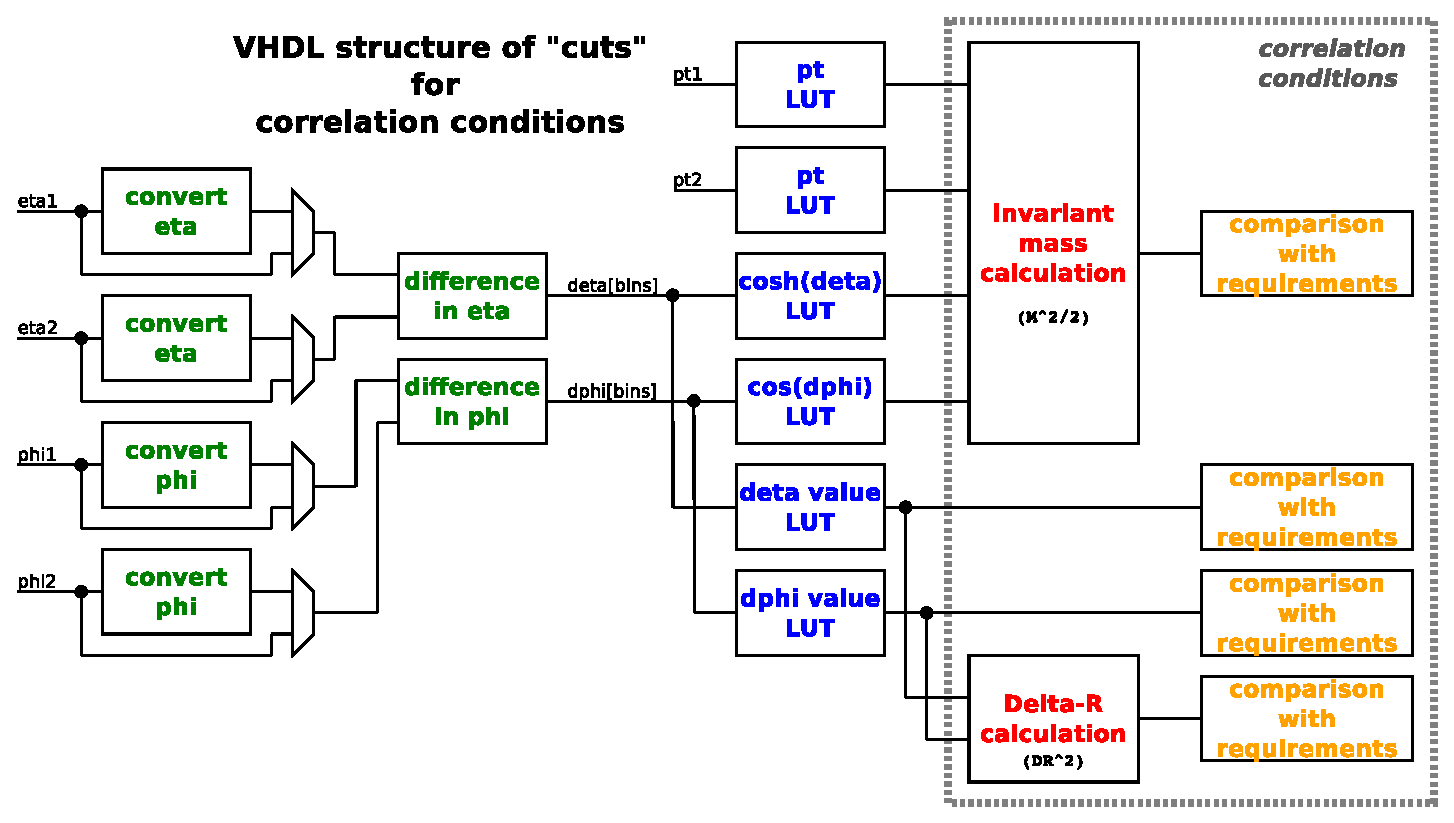
\includegraphics[width=15cm]{figures/scheme_vhdl_cuts_correllation_condition}
\caption{VHDL structure of cuts for correlation conditions} 
\label{fig:gtl:scheme_vhdl_cuts_correllation_condition}
\end{figure}

\paragraph{Calculation of cuts}
\label{sec:gtl:delta_r_calculation}

Calculation of $\Delta\eta$ and $\Delta\varphi$ see section "Calculation of differences in $\eta$ and $\varphi$" (\ref{sec:gtl:calculation_differences}).

\subparagraph{$\Delta$$R$ calculation}
\label{sec:gtl:delta_r_calculation}

The calculation of \textit{$\Delta$$R$} of two objects is done with formula:\\ 

$\Delta$$R=\sqrt{(\eta_1-\eta_2)^2+(\varphi_1-\varphi_2)^2}$.\\

In the TME there are two thresholds for $\Delta$$R$: "greater/equal lower limit" and "less/equal upper limit", given in floating point notation
with one position after decimal point.
The comparison in VHDL is done with $\Delta$$R^2$ (no square root in VHDL), thresholds for $\Delta$$R^2$ are provided by VHDL-Producer.

\subparagraph{Invariant mass calculation}
\label{sec:gtl:inv_mass_calculation}

The calculation of \textit{Invariant mass of two objects} is done with formula:\\

M=$\sqrt{2 pt_1  pt_2 (\cosh(\eta_1-\eta_2)-\cos(\varphi_1-\varphi_2))}$.\\

In the TME there are two thresholds for M: "greater/equal lower limit" and "less/equal upper limit", given in GeV (floating point notation)
with one position after decimal point in even numbers.\footnote{even numbers to get a precision of one position after decimal point after dividion by 2,
because VHDL-Producer calculates thresholds for $\frac{M^2}{2}$, which includes a division by 2.}
The comparison in VHDL is done with $\frac{M^2}{2}$ (no square root in VHDL), thresholds for $\frac{M^2}{2}$ are provided by VHDL-Producer.

\subparagraph{Transverse mass calculation}
\label{sec:gtl:transverse_mass_calculation}

The calculation of \textit{Transverse mass of two objects} is done with formula:\\

M=$\sqrt{2 pt_1 pt_2 (1-\cos(\varphi_1-\varphi_2))}$.\\

In the TME there are two thresholds for M: "greater/equal lower limit" and "less/equal upper limit", given in GeV (floating point notation)
with one position after decimal point in even numbers.
The comparison in VHDL is done with $\frac{M^2}{2}$ (no square root in VHDL), thresholds for $\frac{M^2}{2}$ are provided by VHDL-Producer.

\subparagraph{Two-body pt calculation}
\label{sec:gtl:twobody_pt_calculation}

The calculation of \textit{two-body pt} is done with formula:\\

pt=$\sqrt{pt^2_1 + pt^2_2 + 2  pt_1 pt_2 (\cos(\varphi_1) \cos(\varphi_2) + \sin(\varphi_1) \sin(\varphi_2))}$\\

In the TME there is one threshold for pt, given in GeV (floating point notation) with one position after decimal point.
The comparison in VHDL is done with ${pt^2}$ (no square root in VHDL), threshold for ${pt^2}$ is provided by VHDL-Producer.

\subparagraph{Invariant mass divided by $\Delta$$R$ calculation}
\label{sec:gtl:inv_mass_div_dr_calculation}

The calculation of \textit{Invariant mass divided by $\Delta$$R$ of two objects} is done with formulas:\\

M=$\sqrt{2 pt_1  pt_2 (\cosh(\eta_1-\eta_2)-\cos(\varphi_1-\varphi_2))}$.\\

$\Delta$$R=\sqrt{(\eta_1-\eta_2)^2+(\varphi_1-\varphi_2)^2}$.\\

In the TME there is one threshold for M/$\Delta$$R$: "greater/equal threshold", given in GeV (floating point notation).
The comparison in VHDL is done with $M^2$/(2*$\Delta$$R^2$) (no square root in VHDL), threshold for ($M^2$/2)*(1/$\Delta$$R^2$) is provided by VHDL-Producer.
The values of 1/$\Delta$$R^2$ in VHDL are given by LUTs stored in BRAMs (as ROMs). The addresses of the BRAMs are given by $\Delta\eta$ and $\Delta\varphi$.

\subparagraph{Invariant mass calculation for three objects}
\label{sec:gtl:inv_mass_3_obj_calculation}

The calculation of \textit{Invariant mass calculation for three objects} is done by calculating the invariant mass for all two object combinations and make a summary of three invariant mass of two object combinations. 

\paragraph{Correlation condition modules}
\label{sec:gtl:correlation_condition_modules}

As described in section Correlation conditions (\ref{sec:gtl:correlation_conditions}), correlations of two object types are done. Therefore several modules are provided
with possible correlations (objects 1-objects 2):
\begin{itemize}
\item Correlation condition with calorimeter objects\\(\texttt{calo\_calo\_correlation\_condition.vhd}:
\egamma-\egamma, \egamma-jet, \egamma-tau, jet-jet, jet-tau and tau-tau are possible.)
\item Correlation condition for mass divided by $\Delta$$R$ with calorimeter objects\\(\texttt{calo\_calo\_mass\_div\_dr\_condition.vhd}:
\egamma-\egamma, \egamma-jet, \egamma-tau, jet-jet, jet-tau and tau-tau are possible.)
\item Correlation condition for mass with three objects with calorimeter objects\\(\texttt{calo\_mass\_3\_obj\_condition.vhd}:
\egamma-\egamma, \egamma-jet, \egamma-tau, jet-jet, jet-tau and tau-tau are possible.)
\item Correlation condition with calorimeter objects and muons objects\\(\texttt{calo\_muon\_correlation\_condition.vhd}: \egamma-muon, jet-muon and tau-muon are possible.)
\item Correlation condition with muon objects\\(\texttt{muon\_muon\_correlation\_condition.vhd})
\item Correlation condition with calorimeter objects and \esums (\etm, ET$_{miss}^{HF}$ and \htm only)\\(\texttt{calo\_esums\_correlation\_condition.vhd}: \egamma-etm, jet-etm, tau-etm, \egamma-htm, jet-htm, tau-htm, \egamma-etmhf, jet-etmhf and tau-etmhf are possible.)
\item Correlation condition with muon objects\\(\texttt{muon\_muon\_correlation\_condition.vhd})
\item Correlation condition for mass divided by $\Delta$$R$ with muon objects\\(\texttt{muon\_muon\_mass\_div\_dr\_condition.vhd}
\item Correlation condition for mass with three objects with muon objects\\(\texttt{muon\_mass\_3\_obj\_condition.vhd})
\item Correlation condition with muon objects and \esums (\etm, ET$_{miss}^{HF}$ and \htm only)\\(\texttt{muon\_esums\_correlation\_condition.vhd}: muon-etm, muon-etmhf and muon-htm are possible.)
\end{itemize}

\subparagraph{Overview of possible correlation cuts in conditions}
\label{sec:gtl:overview_correlation_cuts}

The following list gives an overview of possible correlation cuts in conditions:

\begin{itemize}
\item Calo conditions (calo\_conditions.vhd):
\begin{itemize}
\item two-body pt (for double condition)
\end{itemize}
\item Calo conditions overlap removal (calo\_conditions\_orm.vhd):
\begin{itemize}
\item $\Delta\eta$ overlap removal
\item $\Delta\varphi$ overlap removal
\item $\Delta$$R$ overlap removal
\item two-body pt (for double condition)
\end{itemize}
\item Muon conditions (muon\_conditions.vhd):
\begin{itemize}
\item charge correlation
\item two-body pt (for double condition)
\end{itemize}
% % HB 2020-09-11: MJ checks whether it makes sense!
% Muon conditions overlap removal (muon\_conditions\_orm.vhd):
% \begin{itemize}
% \item charge correlation
% \item $\Delta\eta$ overlap removal
% \item $\Delta\varphi$ overlap removal
% \item $\Delta$$R$ overlap removal
% \item two-body pt (for double condition)
% \end{itemize} 
\item Calo calo correlation condition with calo overlap removal (calo\_calo\_calo\_correlation\_orm\_condition.vhd):
\begin{itemize}
\item $\Delta\eta$ overlap removal
\item $\Delta\varphi$ overlap removal
\item $\Delta$$R$ overlap removal
\item $\Delta\eta$
\item $\Delta\varphi$
\item $\Delta$$R$
\item invariant mass
\item two-body pt
\end{itemize} 
\item Calo calo correlation condition (calo\_calo\_correlation\_condition.vhd):
\begin{itemize}
\item $\Delta\eta$
\item $\Delta\varphi$
\item $\Delta$$R$
\item invariant mass
\item two-body pt
\end{itemize}
\item Calo calo correlation condition for invariant mass divided by $\Delta$$R$ (calo\_calo\_mass\_div\_dr\_condition.vhd):
\begin{itemize}
\item invariant mass divided by $\Delta$$R$
\end{itemize}
\item Calo calo correlation condition mass with 3 objects (calo\_mass\_3\_obj\_condition.vhd):
\begin{itemize}
\item invariant mass with 3 objects
\end{itemize} 
\item Calo muon correlation condition (calo\_muon\_correlation\_condition.vhd):
\begin{itemize}
\item $\Delta\eta$
\item $\Delta\varphi$
\item $\Delta$$R$
\item invariant mass
\item two-body pt
\end{itemize} 
\item Calo esums correlation condition (calo\_esums\_correlation\_condition.vhd):
\begin{itemize}
\item $\Delta\varphi$
\item transverse mass
\item two-body pt
\end{itemize}
\item Muon muon correlation condition (muon\_muon\_correlation\_condition.vhd):
\begin{itemize}
\item charge correlation
\item $\Delta\eta$
\item $\Delta\varphi$
\item $\Delta$$R$
\item invariant mass or invariant mass unconstraint pt
\item twobody pt
\end{itemize}
\item Muon muon correlation condition for invariant mass divided by $\Delta$$R$ (muon\_muon\_mass\_div\_dr\_condition.vhd):
\begin{itemize}
\item charge correlation
\item invariant mass divided by $\Delta$$R$
\end{itemize}
\item Muon muon correlation condition mass with 3 objects (muon\_mass\_3\_obj\_condition.vhd):
\begin{itemize}
\item charge correlation
\item invariant mass with 3 objects
\end{itemize} 
\item Muon esums correlation condition (muon\_esums\_correlation\_condition.vhd):
\begin{itemize}
\item $\Delta\varphi$
\item transverse mass
\item twobody pt
\end{itemize}
\end{itemize}

\subparagraph{Calo Calo Correlation condition module}
\label{sec:gtl:calo_calo_correlation_condition_module}

The calo calo correlation condition module contains two "Single object requirement conditions" for different types of calo objects (\egamma, jet or tau) or same type with data from different bunch-crossings as one possible mode and a "Double objects requirement condition" for calo objects of same type and same bunch-crossing as a second mode (selection is done by a parameter in the generic list of \texttt{calo\_calo\_correlation\_condition.vhd} named "same\_bx").\\
In addition there are "Cuts" for differences in $\eta$ (DETA) and $\varphi$ (DPHI), a calculation of $\Delta$$R$ (DR), a calculation of Invariant mass (MASS) and a calculation of two-body pt, see Figure~\ref{fig:gtl:scheme_vhdl_cuts_correllation_condition}.\\
The differences in $\eta$ and $\varphi$ are calculated in bins. These differences in bins are converted to numbers (by LUTs, e.g. \small{EG\_EG\_DIFF\_ETA\_LUT, EG\_EG\_DIFF\_PHI\_LUT}\normalsize, ...), which represents values of differences (multiples of units in $\eta$ and $\varphi$).
These values given in the LUTs are calculated as floating-point values (based on the scales of $\eta$ and $\varphi$), which are multiplied by a factor and truncated to an integer value.
So, in the LUTs we have integer values, the factor is 10\textsuperscript{\tiny{precision}\normalsize}. This "precision" is a parameter given for certain LUTs.\\

\textbf{Remark:} Definitions of scales (see Tables \ref{tab:gtl:calo_eta_scale}, \ref{tab:gtl:calo_phi_scale}, \ref{tab:gtl:muon_eta_scale} and \ref{tab:gtl:muon_phi_scale}):
\begin{itemize}
\item Calorimeter objects:
\item $\eta$ bin width = $\frac{0.087}{2}$ (bin 0 from 0.0 to $\frac{0.087}{2}$)
\item $\phi$ bin width = $\frac{2\pi}{144}$ (bin 0 from 0.0 to $\frac{2\pi}{144}$)
\end{itemize}

The contents of the LUTs for $\cosh(\Delta\eta)$ (\small{EG\_EG\_COSH\_DETA\_LUT}\normalsize, ...) and $\cos(\Delta\varphi)$ (\small{EG\_EG\_COS\_DPHI\_LUT}\normalsize, ...) for Invariant mass (formular see \ref{sec:gtl:inv_mass_calculation}) are created by calculating hyperbolic cosine and cosine, rounding-up at the 3\textsuperscript{rd} position after decimal point, and multiplying by 1000 to get integer values.\footnote{Definition of "\texttt{constant \small{CALO\_INV\_MASS\_COSH\_COS\_PRECISION}\normalsize ..."} in file \texttt{gtl\_pkg.vhd}. Value 1000 from 10\textsuperscript{\tiny{CALO\_INV\_MASS\_COSH\_COS\_PRECISION}}\normalsize.}\\
The contents of the LUTs for $\cos(\varphi)$ (\small{CALO\_COS\_PHI\_LUT}\normalsize) and $\sin(\varphi)$ (\small{CALO\_SIN\_PHI\_LUT}\normalsize) for two-body pt
(formular see \ref{sec:gtl:twobody_pt_calculation}) are created by calculating cosine and sine, rounding-up at the 3\textsuperscript{rd} position after decimal point and 
multiplying by 1000 to get integer values.\\
The condition is complied, if at least one comparison between object parameters and requirements is valid for the both "Single object requirement condition" or the "Double objects requirement condition" and the results of selected "Cuts" are inside of a range (upper and lower limit) or greater/eual a threshold (e.g. for two-body pt).
This limits are parts of the "generic" list of the entity declaration of the module and are expressed in hex notation. The limits for DETA and DPHI
are expressed with a precision of 3\textsuperscript{rd} position after decimal point, for DR, MASS and two-body pt with 1\textsuperscript{st} position after decimal point.

\subparagraph{Calo Calo Correlation condition module for invariant mass divided by $\Delta$$R$}
\label{sec:gtl:calo_calo_correlation_condition_module_mass_div_dr}

\subparagraph{Calo Calo Correlation condition module for invariant mass with 3 objects}
\label{sec:gtl:calo_calo_correlation_condition_module_mass_3_obj}

\subparagraph{Calo Calo Overlap Remover Correlation condition module}
\label{sec:gtl:calo_calo_overlap_remover_condition_module}

The Calo Calo Overlap Remover Correlation conditions consits of two modes. One with a Calo Calo Correlation condition with "Double objects requirement condition" for calo objects of same type and same bunch-crossing (\ref{sec:gtl:calo_calo_correlation_condition_module}) and a single condition for a different calo object type (can have different bunch-crossing too). There has to be at least one correlation cut for the objects of "Double objects requirement condition" and a correlation cut for overlap removal between objects (one or more cut(s) of $\Delta\eta$, $\Delta\varphi$ and $\Delta$$R$)
of different object types ("2plus1"). A second mode ("1plus1") with a Calo Calo Correlation condition with a single condition and a different calo object type (can have different bunch-crossing too) also with a single condition. There has to be at least one correlation cut for the different objects (e.g. invariant mass) and a correlation cut for overlap removal between the objects (one or more cut(s) of $\Delta\eta$, $\Delta\varphi$ and $\Delta$$R$). 

\subparagraph{Calo Muon Correlation condition module}
\label{sec:gtl:calo_muon_correlation_condition_module}

The calo muon correlation condition module contains a "Single object requirement condition" for one type of calo objects (\egamma, jet or tau) and a "Single object requirement condition" for muon objects.
In addition there are "Cuts" for differences in $\eta$ (DETA) and $\varphi$ (DPHI), a calculation of $\Delta$$R$ (DR), a calculation of Invariant mass (MASS) and a calculation of two-body pt, see Figure~\ref{fig:gtl:scheme_vhdl_cuts_correllation_condition}.\\
The differences in $\eta$ and $\varphi$ are calculated in bins. These differences in bins are converted to numbers (by LUTs, e.g. \small{EG\_MU\_DIFF\_ETA\_LUT, EG\_MU\_DIFF\_PHI\_LUT}\normalsize, ...), which represents values of differences (multiples of units in $\eta$ and $\varphi$).
These values given in the LUTs are calculated as floating-point values (based on the scales of $\eta$ and $\varphi$), which are multiplied by a factor and truncated to an integer value.
So, in the LUTs we have integer values, the factor is 10\textsuperscript{\tiny{precision}\normalsize}. This "precision" is a parameter given for certain LUTs.\\
Because of the different scales of calorimeter and muon objects in $\eta$ and $\varphi$, there are LUTs for conversion the calorimeter bins to muon bins (in \texttt{gtl\_pkg.vhd}:
 e.g. \small{EG\_ETA\_CONV\_2\_MUON\_ETA\_LUT}\normalsize and \small{EG\_PHI\_CONV\_2\_MUON\_PHI\_LUT}\normalsize).\\\\
\textbf{Remark:}\\
The center value of bins are used as reference value for conversion.
The content of \small{EG\_ETA\_CONV\_2\_MUON\_ETA\_LUT}\normalsize is calculated with formular:\\ "converted-calo-eta[bin] = calo-eta[bin] $\times$ 4 + 2",\\
of \small{EG\_PHI\_CONV\_2\_MUON\_PHI\_LUT}\normalsize with formular:\\
"converted-calo-phi[bin] = calo-phi[bin] $\times$ 4 + 2".\\
The conversion calculations are preliminary, others may be proposed.\\\\
Definitions of scales (see Tables \ref{tab:gtl:calo_eta_scale}, \ref{tab:gtl:calo_phi_scale}, \ref{tab:gtl:muon_eta_scale} and \ref{tab:gtl:muon_phi_scale}):
\begin{itemize}
\item Calorimeter objects:
\begin{itemize}
\item $\eta$ bin width = $\frac{0.087}{2}$ (bin 0 from 0.0 to $\frac{0.087}{2}$)
\item $\phi$ bin width = $\frac{2\pi}{144}$ (bin 0 from 0.0 to $\frac{2\pi}{144}$)
\end{itemize}
\item Muon objects:
\begin{itemize}
\item $\eta$ bin width = $\frac{0.087}{8}$ (bin 0 from \small{0.5}$\times\frac{-0.087}{8}$ to \small{0.5}$\times\frac{+0.087}{8}$)
\item $\phi$ bin width = $\frac{2\pi}{576}$ (bin 0 from 0.0 to $\frac{2\pi}{576}$)
\end{itemize}
\end{itemize}

\begin{figure}[htb]
\centering
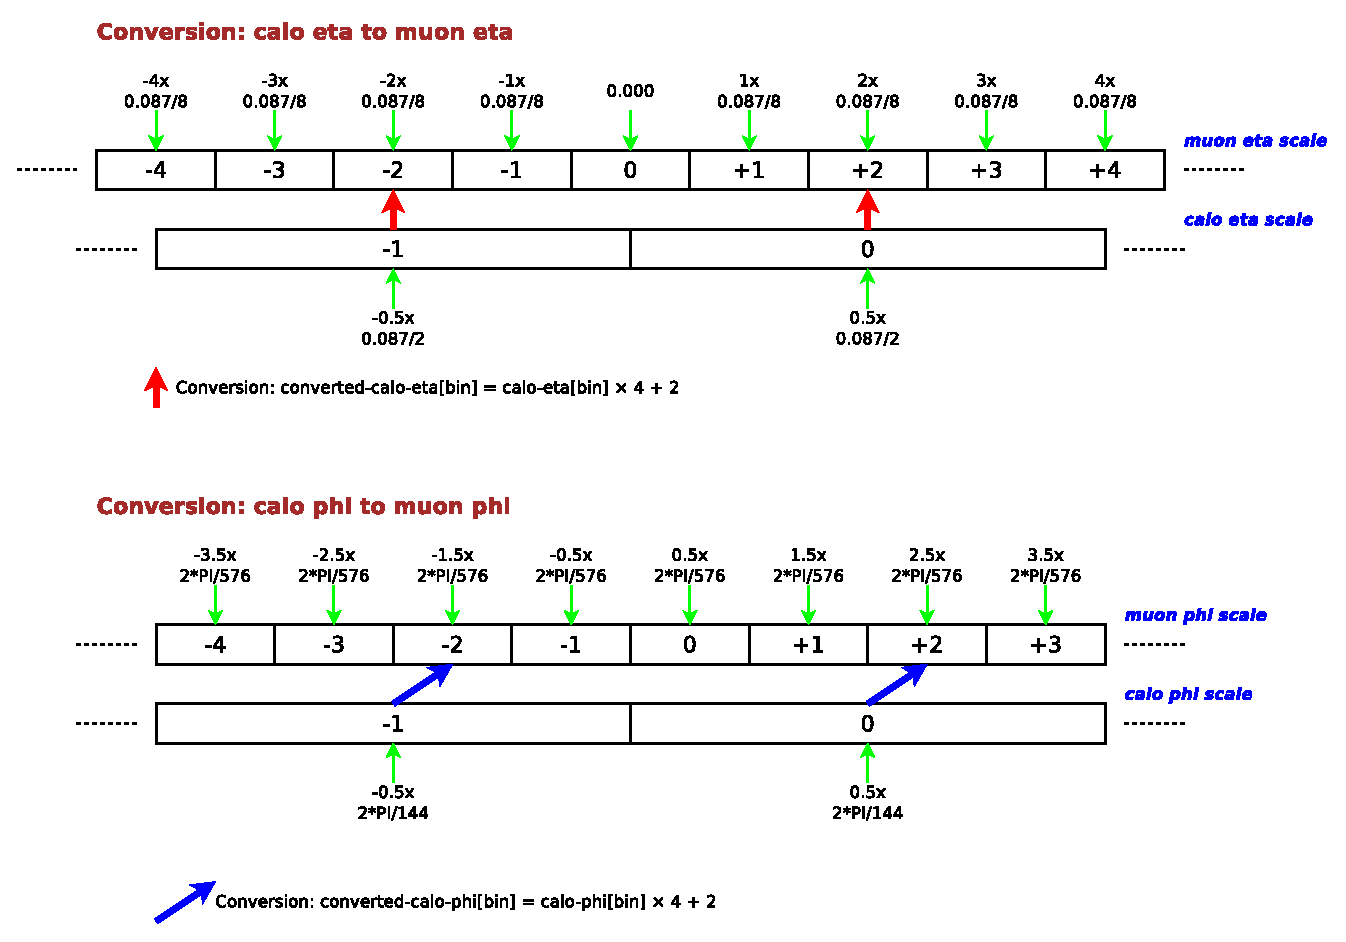
\includegraphics[width=15cm]{figures/convert_scheme_calo_2_muon_eta_phi}
\caption{Conversion of calorimeter $\eta$ and $\varphi$ to muon scales} 
\label{fig:gtl:convert_scheme_calo_2_muon_eta_phi}
\end{figure}

The contents of the LUTs for $\cosh(\Delta\eta)$ (\small{EG\_MUON\_COSH\_DETA\_LUT}\normalsize, ...) and $\cos(\Delta\varphi)$ (\small{EG\_MUON\_COS\_DPHI\_LUT}\normalsize, ...) for Invariant mass (formular see \ref{sec:gtl:inv_mass_calculation}) are created by calculating hyperbolic cosine and cosine, rounding-up at the 4\textsuperscript{th} position after decimal point, and multiplying by 10000(10\textsuperscript{\tiny{CALO\_MUON\_INV\_MASS\_COSH\_COS\_PRECISION}}\normalsize) to get integer values.\footnote{Definition of "\texttt{constant \small{CALO\_MUON\_INV\_MASS\_COSH\_COS\_PRECISION}\normalsize} ...", "\texttt{constant \small{EG\_ETA\_CONV\_2\_MUON\_ETA\_LUT}\normalsize} ..." and "\texttt{constant \small{EG\_PHI\_CONV\_2\_MUON\_PHI\_LUT}\normalsize} ..." in file \texttt{gtl\_pkg.vhd}.}\\
The contents of the LUTs for $\cos(\varphi)$ (\small{CALO\_COS\_PHI\_LUT and MUON\_COS\_PHI\_LUT}\normalsize) and $\sin(\varphi)$ (\small{CALO\_SIN\_PHI\_LUT and MUON\_SIN\_PHI\_LUT}\normalsize) for two-body pt (formular see \ref{sec:gtl:twobody_pt_calculation}) are created by calculating cosine and sine, rounding-up at the 3\textsuperscript{rd} position after decimal point, and multiplying by 1000 to get integer values.\\
The condition is complied, if at least one comparison between object parameters and requirements is valid for the both "Single object requirement condition" and the results of selected "Cuts" are inside of a range (upper and lower limit) or greater/eual a threshold (e.g. for two-body pt). 
This limits are parts of the "generic" list of the entity declaration of the module and are expressed in hex notation. The limits for DETA and DPHI
are expressed with a precision of 3\textsuperscript{rd} position after decimal point, for DR, MASS and two-body pt with 1\textsuperscript{st} position after decimal point.


\subparagraph{Muon Muon Correlation condition module}
\label{sec:gtl:muon_muon_correlation_condition_module}

The muon muon correlation condition module contains two "Single object requirement conditions" for data from different bunch-crossings as one possible mode
and a "Double objects requirement condition" for muon objects at same bunch-crossing as a second mode (selection is done by a parameter in the
generic list of \texttt{muon\_muon\_correlation\_condition.vhd} named "same\_bx"). In the case of a "Double objects requirement condition", requirements for "requested charge correlations" are used and a muon charge correlation module (see \ref{sec:gtl:muon_charge_correlation_module}) is required.\\
In addition there are "Cuts" for differences in $\eta$ (DETA) and $\varphi$ (DPHI), a calculation of $\Delta$$R$ (DR), a calculation of Invariant mass with pt or of Invariant mass with unconstrained pt (MASS), a calculation of two-body pt.\\
The differences in $\eta$ and $\varphi$ are calculated in bins. These differences in bins are converted to numbers (by LUTs, e.g. \small{MUON\_MUON\_DIFF\_ETA\_LUT, MUON\_MUON\_DIFF\_PHI\_LUT}\normalsize), which represents values of differences (multiples of units in $\eta$ and $\varphi$).
These values given in the LUTs are calculated as floating-point values (based on the scales of $\eta$ and $\varphi$), which are multiplied by a factor and truncated to an integer value.
So, in the LUTs we have integer values, the factor is 10\textsuperscript{\tiny{precision}\normalsize}. This "precision" is a parameter given for certain LUTs.\\

\textbf{Remark:} Definitions of scales (see Tables \ref{tab:gtl:muon_eta_scale} and \ref{tab:gtl:muon_phi_scale}):
\begin{itemize}
\item Muon objects:
\item $\eta$ bin width = $\frac{0.087}{8}$ (bin 0 from \small{0.5}$\times\frac{-0.087}{8}$ to \small{0.5}$\times\frac{+0.087}{8}$)
\item $\phi$ bin width = $\frac{2\pi}{576}$ (bin 0 from 0.0 to $\frac{2\pi}{576}$)
\end{itemize}

The contents of the LUTs for $\cosh(\Delta\eta)$ (\small{MUON\_MUON\_COSH\_DETA\_LUT}\normalsize) and $\cos(\Delta\varphi)$ (\small{MUON\_MUON\_COS\_DPHI\_LUT}\normalsize) for Invariant mass (formular see \ref{sec:gtl:inv_mass_calculation}) are created by calculating hyperbolic cosine and cosine, rounding-up at the 4\textsuperscript{th} position after decimal point, and multiplying by 10000 to get integer values.\footnote{Definition of "\texttt{constant \small{MUON\_INV\_MASS\_COSH\_COS\_PRECISION}\normalsize"} in file \texttt{gtl\_pkg.vhd}. Value 10000 from 10\textsuperscript{\tiny{MUON\_INV\_MASS\_COSH\_COS\_PRECISION}}\normalsize.}\\
The contents of the LUTs for $\cos(\varphi)$ (\small{MUON\_COS\_PHI\_LUT}\normalsize) and $\sin(\varphi)$ (\small{MUON\_SIN\_PHI\_LUT}\normalsize) for two-body pt 
(formular see \ref{sec:gtl:twobody_pt_calculation}) are created by calculating cosine and sine, rounding-up at the 3\textsuperscript{rd} position after decimal point,
and multiplying by 1000 to get integer values.\\
The condition is complied, if at least one comparison between object parameters and requirements is valid for the both "Single object requirement condition" or the "Double objects requirement condition" and the results of selected "Cuts" are inside of a range (upper and lower limit) or greater/eual a threshold (e.g. for two-body pt).
This limits are parts of the "generic" list of the entity declaration of the module and are expressed in hex notation. The limits for DETA and DPHI
are expressed with a precision of 3\textsuperscript{rd} position after decimal point, for DR and MASS with 1\textsuperscript{st} position after decimal point.

\subparagraph{Muon Muon Correlation condition module for invariant mass divided by $\Delta$$R$}
\label{sec:gtl:muon_muon_correlation_condition_module_mass_div_dr}

\subparagraph{Muon Muon Correlation condition module for invariant mass with 3 objects}
\label{sec:gtl:muon_muon_correlation_condition_module_mass_3_obj}

\subparagraph{Calo Esums Correlation condition module}
\label{sec:gtl:calo_esums_correlation_condition_module}

The calo esums correlation condition module contains two "Single object requirement conditions", one of calo objects (\egamma, jet or tau) and one of esums (\etm, ET$_{miss}^{HF}$ or \htm).\\
In addition there are "Cuts" for differences in $\varphi$ (DPHI) or a calculation of mass (MASS) for Transverse mass or Transverse mass with two-body pt.\\
The differences in $\varphi$ are calculated in bins. 
These differences in bins are converted to numbers (by LUTs, e.g. \small{EG\_ETM\_DIFF\_PHI\_LUT}\normalsize, ...),
which represents values of differences (multiples of units in $\varphi$).
These values given in the LUTs are calculated as floating-point values (based on the scales of $\varphi$), which are multiplied by a factor and truncated to an integer value.
So, in the LUTs we have integer values, the factor is 10\textsuperscript{\tiny{precision}\normalsize}.\\

The contents of the LUTs $\cos(\Delta\varphi)$ (\small{EG\_ETM\_COS\_DPHI\_LUT}\normalsize, ...) for Transverse mass (formular see \ref{sec:gtl:transverse_mass_calculation}) 
are created by calculating cosine, rounding-up at the 3\textsuperscript{rd}
position after decimal point and multiplying by 1000 to get integer values.\footnote{Definition of "\texttt{constant \small{CALO\_INV\_MASS\_COSH\_COS\_PRECISION}\normalsize ..."} in file \texttt{gtl\_pkg.vhd}.
1000 from 10\textsuperscript{\tiny{CALO\_INV\_MASS\_COSH\_COS\_PRECISION}}\normalsize.}\\
The contents of the LUTs for $\cos(\varphi)$ (\small{CALO\_COS\_PHI\_LUT}\normalsize) and $\sin(\varphi)$ (\small{CALO\_SIN\_PHI\_LUT}\normalsize) for two-body pt 
(formular see \ref{sec:gtl:twobody_pt_calculation}) are created by calculating cosine and sine, rounding-up at the 3\textsuperscript{rd} position after decimal point and multiplying by 1000 to get integer values.\\
The condition is complied, if at least one comparison between object parameters and requirements is valid for the both "Single object requirement condition"
and the results of selected "Cuts" are inside of a range (upper and lower limit).
This limits are parts of the "generic" list of the entity declaration of the module and are expressed in hex notation. The limits for DPHI
are expressed with a precision of 3\textsuperscript{rd} position after decimal point, for MASS with 1\textsuperscript{st} position after decimal point.

\subparagraph{Muon Esums Correlation condition module}
\label{sec:gtl:muon_esums_correlation_condition_module}

The muon esums correlation condition module contains two "Single object requirement conditions", one of muon objects and one of esums (\etm, ET$_{miss}^{HF}$ or \htm).\\
In addition there are "Cuts" for differences in $\varphi$ (DPHI) or a calculation of mass (MASS) for Transverse mass or Transverse mass with two-body pt.\\
The differences in $\varphi$ are calculated in bins. These differences in bins are converted to numbers (by LUTs, e.g. \small{MUON\_ETM\_DIFF\_PHI\_LUT}\normalsize, ...),
which represents values of differences (multiples of units in $\varphi$).
These values given in the LUTs are calculated as floating-point values (based on the scales of $\varphi$), which are multiplied by a factor and truncated to an integer value.
So, in the LUTs we have integer values, the factor is 10\textsuperscript{\tiny{precision}\normalsize}.\\
Because of the different scales of muon objects and esums in $\varphi$, there are LUTs for conversion the esums bins to muon bins (in \texttt{gtl\_pkg.vhd}:
 e.g. \small{ETM\_PHI\_CONV\_2\_MUON\_PHI\_LUT}\normalsize).\\\\
\textbf{Remark:}\\
The center value of bins are used as reference value for conversion.
The content of LUT is calculated with formular:\\
"converted-esums-phi[bin] = esums-phi[bin] $\times$ 4 + 2"\\ (see Figure~\ref{fig:gtl:convert_scheme_calo_2_muon_eta_phi}).
The conversion calculations are preliminary, others may be proposed.\\\\
Definitions of scales:
\begin{itemize}
\item \etm, ET$_{miss}^{HF}$ or \htm:
\begin{itemize}
\item $\phi$ bin width = $\frac{2\pi}{144}$ (bin 0 from 0.0 to $\frac{2\pi}{144}$)
\end{itemize}
\item Muon objects:
\begin{itemize}
\item $\phi$ bin width = $\frac{2\pi}{576}$ (bin 0 from 0.0 to $\frac{2\pi}{576}$)
\end{itemize}
\end{itemize}

The contents of the LUTs for $\cos(\Delta\varphi)$ (\small{MU\_ETM\_COS\_DPHI\_LUT}\normalsize, ...) for Transverse mass (formular see \ref{sec:gtl:transverse_mass_calculation}) 
are created by calculating cosine, rounding-up at the 4\textsuperscript{th} 
position after decimal point and multiplying by 10000 (10\textsuperscript{\tiny{MU\_ETM\_COSH\_COS\_PRECISION}}\normalsize) to get integer values.\footnote{Definition of 
"\texttt{constant \small{MU\_ETM\_COSH\_COS\_PRECISION}\normalsize} ..." and "\texttt{constant \small{CALO\_PHI\_CONV\_2\_MUON\_PHI\_LUT}\normalsize} ..." in file \texttt{gtl\_pkg.vhd}.}\\
The contents of the LUTs for $\cos(\varphi)$ (\small{CALO\_COS\_PHI\_LUT and MUON\_COS\_PHI\_LUT}\normalsize) and $\sin(\varphi)$ (\small{CALO\_SIN\_PHI\_LUT and MUON\_SIN\_PHI\_LUT}\normalsize) for two-body pt 
(formular see \ref{sec:gtl:twobody_pt_calculation}) are created by calculating cosine and sine, rounding-up at the 3\textsuperscript{rd} position after decimal point and multiplying by 1000 to get integer values.\\
The condition is complied, if at least one comparison between object parameters and requirements is valid for the both "Single object requirement condition"
and the results of selected "Cuts" are inside of a range (upper and lower limit).
This limits are parts of the "generic" list of the entity declaration of the module and are expressed in hex notation. The limits for DPHI
are expressed with a precision of 3\textsuperscript{rd} position after decimal point, for MASS with 1\textsuperscript{st} position after decimal point.

\subsubsection{External Conditions}
\label{sec:gtl:external_conditions}
Maximal 256 External Conditions are possible in \gt. They are provided as inputs in the Algorithms logic of \ugtl.
External Conditions will include the "Technical Trigger" of the legacy system.

\subsubsection{Algorithms logic}
\label{sec:gtl:algorithms_logic}

The outputs of all the instantiated conditions are combined in the Algorithms logic with boolean algebra given by TME for every single Algorithm. These Algorithms are registered and provided
as inputs for \fdl.

\clearpage



%------------------------------------------------------------------------------
%
% Repository path   : $HeadURL: https://hbergauer@forge.hephy.oeaw.ac.at/scm/svn/project-cmstrigger/GlobalTriggerUpgrade/doc/latex/gt-mp7-firmware-specification/content/fdl.tex $
% Last committed    : $Revision: 4475 $
% Last changed by   : $Author: hbergauer $
% Last changed date : $Date: 2018-01-19 10:02:12 +0100 (Fri, 19 Jan 2018) $
% Description       : Specification of Final Decision Logic
% ------------------------------------------------------------------------------
\section{Final Desicion Logic}\label{sec:fdl:ufdl}

The Final Desicion Logic (\ufdl) firmware contains algo-bx-masks, suppression of algos caused by calibration trigger, prescalers, veto-masks and rate-counters
("before prescalers", "after prescalers" and "post dead time") for each Algorithm and the local \finor- and veto-logic.

\begin{figure}[htb]
\centering
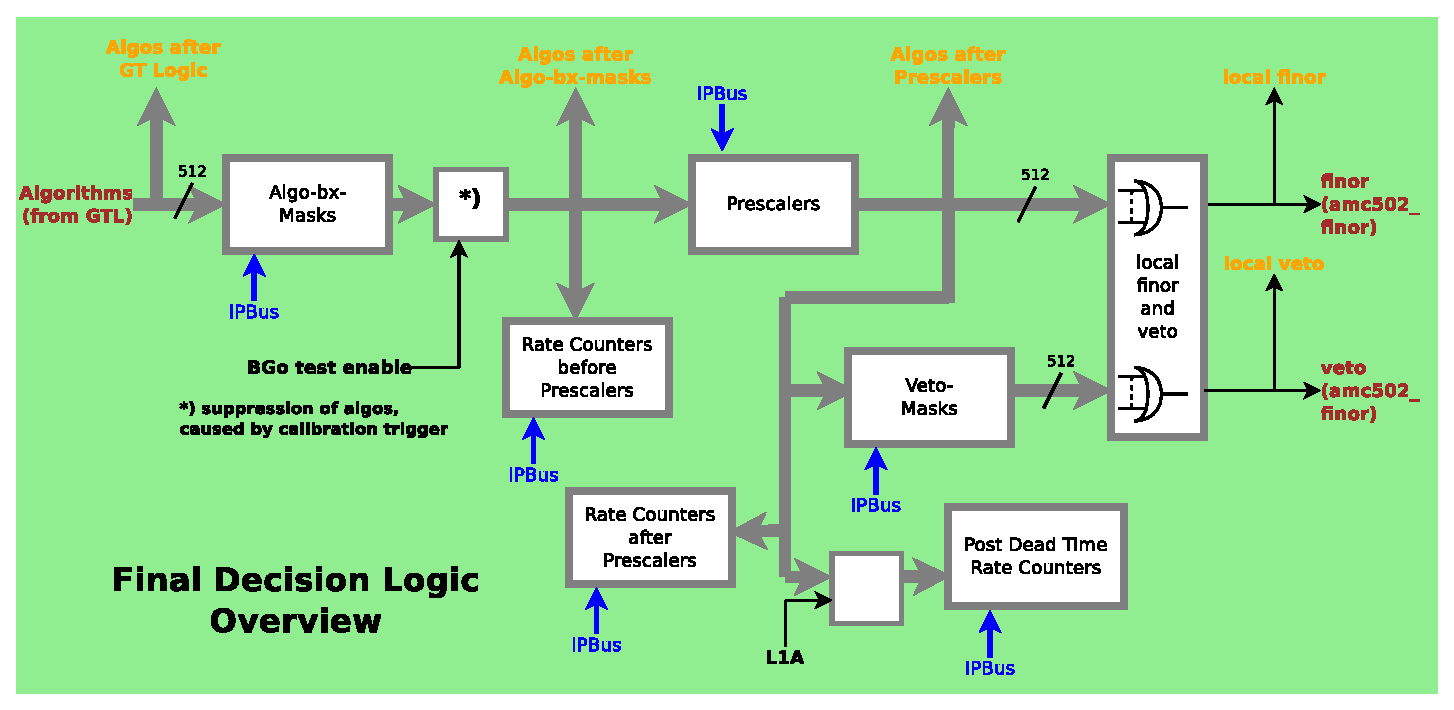
\includegraphics[width=15cm]{figures/mFDL_firmware}
\caption{\ufdl firmware v1.0.1} 
\label{fig:fdl:mFDL_firmware}
\end{figure}

\subsection{\ufdl Interface}
\label{sec:fdl:ufdl_interface}

%\textit{under construction ...}

\textbf{Inputs:}
\begin{itemize}
\item Algorithms from \ugtl
\item IPBus interface (for registers, counters and memories)
\item LHC-clock
\item Reset signal
\item BC0, BGo test-enable, L1A
% \item Indication of LHC gap
\item Begin of lumi-section
% \item Bx-nr for algo-bx-masks memory
\end{itemize}
\textbf{Outputs:}
\begin{itemize}
% \item Status information of \ufdl
\item Prescale factor set index to \rop
\item Algorithms after GTLogic to \rop
\item Algorithms after algo-bx-masks to \rop
\item Algorithms after prescalers to \rop
\item Algorithms after \finor-masks to \rop
\item Local \finor to \rop
\item Local veto to \rop
\item Local \finor with veto to \rop
\item Local \finor to mezzanine
\item Local veto to mezzanine
\item Local \finor with veto to mezzanine
\end{itemize}

\subsection{MP7 \finor hardware solution}

%% Text, figures and tables moved to com-hardware.tex
The firmware of \ufdl in this document is based on a hardware configuration with maximum 6 \ugt modules. 
% A proposed hardware solution for \finor is documented in \ref{sec:com-hard:hw_config_finor_mp7}.

\subsection{Data flow}
\label{sec:fdl:data_flow}

\begin{figure}[htb]
\centering
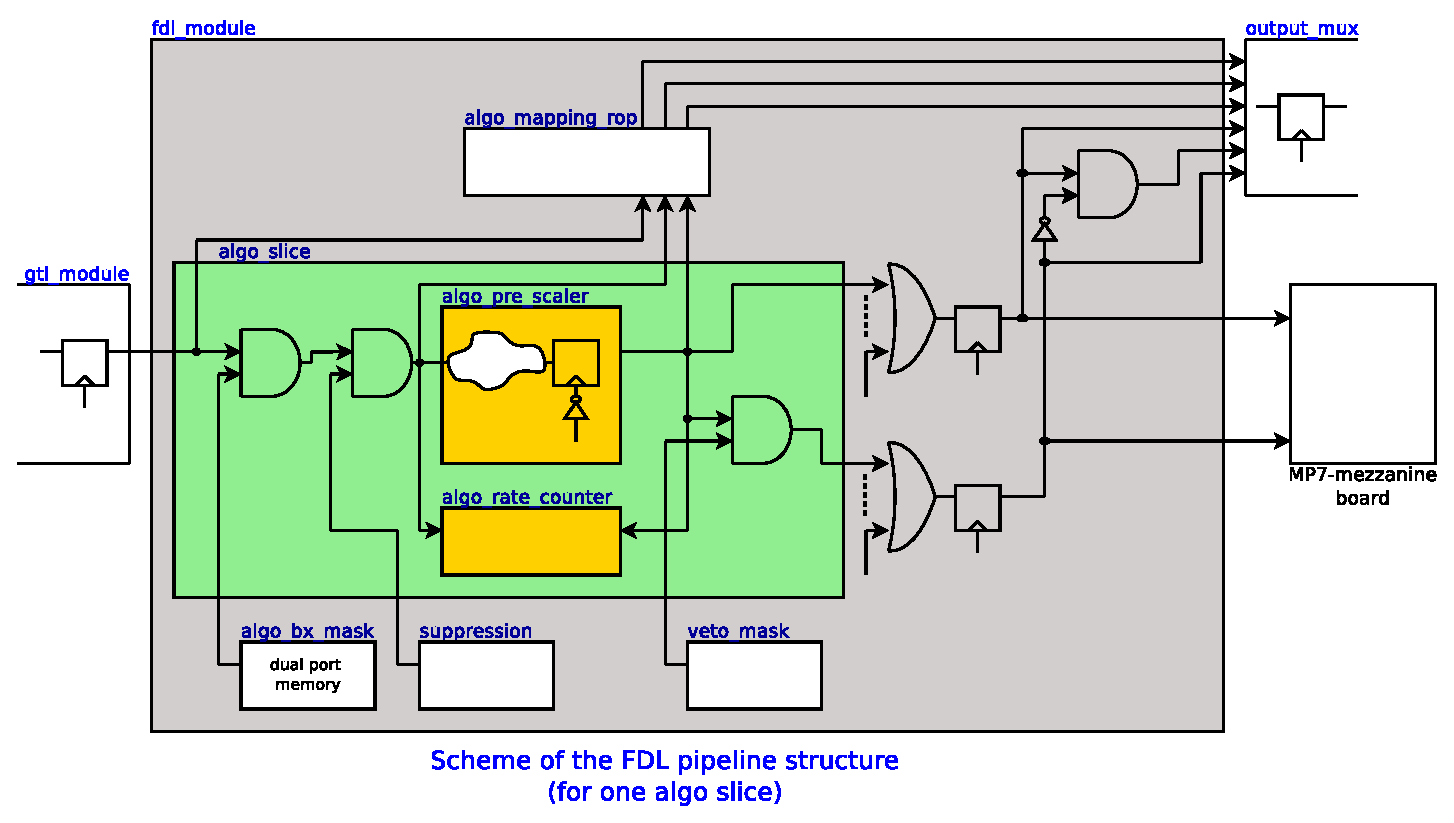
\includegraphics[width=15cm]{figures/fdl_pipeline}
\caption{\ufdl pipeline v1.0.1} 
\label{fig:fdl:mFDL_pipeline}
\end{figure}

Every Algorithm, in total 512 coming from \ugtl, passes a algo-bx-mask, the logic for suppression of algos caused by calibration trigger and a prescaler, which reduces the trigger rate by a given factor. Prescaled Algorithms signals are combined to a local final-or-signal (\finor).
For every Algorithm there is a rate-counter before prescaler and after prescaler, which are incremented by LHC-clock if the Algorithm is true. In addition there are post-dead-time counters, one for each Algorithm, which are incremented,
if the Algorithm and the L1A-signal are true at the same bunch-crossing.
% Algorithms signals after \finor-masks selected by veto-mask disable the total \finor-signal, if one of the selected Algorithm is true. The total \finor-signal is provided to TCDS. 
Algorithms after GTLogic, after algo-bx-masks, after prescalers, the local \finor- and local veto-signal are provided for read-out-record.\\
If there are not enough firmware resources in one \ugt board, more boards could be used. Therefore the 512 Algorithms are partitioned by TME. TME will set the number of Algorithms as
constant in the package module \texttt{gtl\_pkg.vhd}. This means \ugtl and \ufdl firmware considered as a unit for synthesis. In the case of more \ugt boards, the local \finor and local veto are routed via
a mezzanine board on MP7 (located on "General Purpose I/O connector") to the FINOR-AMC502 module, where the total \finor is created and send to TCDS.\\
A mapping for Algorithms is provided, to give flexibility for setting the index of Algorithms:
\begin {itemize}
\item creating a mapping instance (algo\_mapping\_rop.vhd) over TME (see \ref{sec:gtl:algo_mapping_tme}), this component will be instantiated in fix part of FDL, and new calculation will done each time over TME.
\item TME delivers just the number of Algorithms, which will be built on each card.
% \item TME additionally deliver the mapping process, in order FDL and IPBus, ROP know, which algorithm is at which address. 
\item from FDL point of view, FDL see incremented number of Algorithms indexes, \eg 0, 1, 2, which is \eg 69, 200, 300.
\item TME should take care of assignment of each Algorithm to a number, that means if in card 1 algo\_59 is defined, nobody allows to produce the same number again.
\end {itemize}
% A software which manages these partitioned Algorithms for setting prescale factors, reading rate-counters and other accesses has to be developed.\\

\subsection{Main parts}

The top-of-hierarchy module (\texttt{fdl\_module.vhd}) contains 
\begin {itemize}
\item version registers
% \item a control register
\item a command pulse register
% \item a status register
\item prescalers for all Algorithms
\item registers for prescale factors
\item register for prescale factor set index
\item rate-counters for all Algorithms, finor, veto, L1A and post-dead-time
\item read only registers for rate-counter values
\item algo-bx-masks for all Algorithms
\item \finor-masks for all Algorithms
\item veto-masks for all Algorithms
\item the \finor-logic
\end {itemize}

% \subsubsection{Reset structure}
% \label{sec:fdl:reset_structure}
% 
% \textit{under construction ...}
% 
\subsubsection{Registers and memories}
\label{sec:fdl:reg_mem}

All registers and memories are 32 bits wide. (A first draft of the definition of the relative addresses is shown in Table~\ref{tab:ufdl_register_map}.)

\begin {itemize}
\item Dual-port memories for the algo-bx-masks are implemented. For each Algorithm there is a mask bit at every bunch crossing of one orbit. Therefore in total memories of 4096 x 512 bits
are implemented. Because of the 32 bit data interface, 16 memories each with a size of 4096 x 32 bits are instantiated.
\item Read-only registers for the value of rate-counters (before and after prescalers, post-dead-time counters) are implemented, 512 registers, one for every Algorithm. Rate-counter value has 32 bits.
\item Registers for prescale factor of the prescalers are implemented, 512 registers, one for every Algorithm. A prescale factor value has 24 bits.
\item Registers for masks (finor- and veto-masks) are implemented, 512 registers.
\item One register for prescale factors set index is implemented. This register contains a value, which is unique for a given set of prescale factors. The content of this register is
part of \record.
\item One register for command pulses is implemented. One bit of this register (bit 0) is used for "setting the request signal for updating prescale factors high", which enables, that the prescale factors and the prescale factor set index
are loaded at the begin of a luminosity segment period. (Other bits are not defined yet.)
\item One control register is implemented (the content has to be defined).
% \item One register for status information is implemented. The content has to be defined.
\item 32 register for L1 Trigger Menu name for \ugtl is implemented.
\item 4 register for L1 Trigger Menu UUID for \ugtl is implemented.
\item One register for L1 Trigger Menu compiler version is implemented.
\item One register for \ufdl firmware version is implemented.
\item One register for \ugtl firmware (fixed code) version is implemented.
\end {itemize}

\paragraph{Register map}
\label{sec:fdl:reg_map}
The register map for \ufdl has a base address of \verb|0x90000000|.

% % HB 2016-11-03: inserted "longtable"
\begin{longtable}{c p{.4\columnwidth} c p{.33\columnwidth}}
\caption{\ufdl register map}\\
\hline 
Offset & {Register name} & {Access} & {Description}\\
\hline
\hline
\endhead
0x90000000 & \verb|Algo BX masks(0)| & r/w & 4096 memory addresses of algo-bx-masks for Algorithms 0-31.\\
0x90001000 & \verb|Algo BX masks(1)| & r/w & 4096 memory addresses of algo-bx-masks for Algorithms 32-63.\\
... & ... & ... & ...\\
0x9000F000 & \verb|Algo BX masks(15)| & r/w & 4096 memory addresses of algo-bx-masks for Algorithms 480-511.\\
0x90010000 & \verb|Rate counter before prescaler| & r & 512 read-only registers for rate-counter values before prescalers.\\
0x90010200 & \verb|Prescale factors| & r/w & 512 registers for prescale factors.\\
0x90010400 & \verb|Rate counter after prescaler| & r & 512 read-only registers for rate-counter values after prescalers.\\
0x90010600 & \verb|Rate counter post-dead-time| & r & 512 read-only registers for post-dead-time rate-counter values.\\
0x90010800 & \verb|Masks| & r/w & 512 registers for finor-masks and veto-masks. Bit 0 = finor-mask, bit 1 = veto-mask.\\
0x90091880 & \verb|Prescale factors set index| & r/w & Register for prescale factors set index.\\
% 0x90091888 & \verb|Control| & r/w & Register for control signals (content has to be defined !!!).\\
0x900918C0 & \verb|L1tm name| & r & 32 registers for L1 Trigger Menu name for \ugtl.\\
0x900918E0 & \verb|L1tm uuid| & r & 4 registers for L1 Trigger Menu UUID for \ugtl.\\
0x900918E4 & \verb|L1tm compiler version| & r & Register for L1 Trigger Menu compiler version.\\
0x900918E5 & \verb|GTL FW version| & r & Register for firmware version of \ugtl VHDL code.\\
0x900918E6 & \verb|FDL FW version| & r & Register for firmware version of \ufdl VHDL code.\\
0x900918E7 & \verb|L1tm FW uuid| & r & 4 registers for L1 Trigger Menu FW UUID for \ugtl.\\
0x900918EB & \verb|SVN revision number| & r & Register for SVN revision number.\\
0x900918EC & \verb|L1tm uuid hash| & r & Register for L1 Trigger Menu UUID hash for \ugtl.\\
0x900918ED & \verb|L1tm FW uuid hash| & r & Register for L1 Trigger Menu FW UUID hash for \ugtl.\\
0x900918EE & \verb|Module ID| & r & Register for Module ID of L1 Trigger Menu.\\
0x90091900 & \verb|Command Pulses| & r/w & Register for command pulses.\\
0x90091980 & \verb|Rate counter finor| & r & One read-only registers for finor rate-counter value.\\
0x90092200 & \verb|L1A latency delay| & r/w & Register for L1A latency delay value (used for post-dead-time counter).\\
0x90093000 & \verb|Rate counter L1A| & r & One read-only registers for L1A rate-counter value.\\
0x90094000 & \verb|Rate counter veto| & r & One read-only registers for veto rate-counter value.\\
0x90095000 & \verb|Current prescale set index| & r & Read-only register for prescale factors set index, which was "updated" with begin of current lumi-section ("prescale\_factors\_set\_index\_reg\_updated(0)" in VHDL).\\
0x90095001 & \verb|Previous prescale set index| & r & Read-only register for prescale factors set index, which was "updated" with begin of previous lumi-section for monitoring "prescale\_factors\_set\_index\_reg\_updated(1)" in VHDL).\\
0x90096000 & \verb|Calibration trigger gap| & r/w & Register for begin and end (in Bx) of calibration trigger gap.\\
\hline
\label{tab:ufdl_register_map}
\end{longtable}

% \medskip
% \begin{table}[htdp]
% \footnotesize
% \begin{center}
% \begin{tabular}{c p{.4\columnwidth} c p{.33\columnwidth}}
% \toprule
% Offset & {Register name} & {Access} & {Description}\\
% \midrule      
% 0x90000000 & \verb|Algo BX masks(0)| & r/w & 4096 memory addresses of algo-bx-masks for Algorithms 0-31.\\
% % 0x90001000 & \verb|Algo BX masks(1)| & r/w & 4096 memory addresses of algo-bx-masks for Algorithms 32-63.\\
% ... & ... & ... & ...\\
% 0x9000F000 & \verb|Algo BX masks(15)| & r/w & 4096 memory addresses of algo-bx-masks for Algorithms 480-511.\\
% 0x90010000 & \verb|Rate counter before prescaler| & r & 512 read-only registers for rate-counter values before prescalers.\\
% 0x90010200 & \verb|Prescale factors| & r/w & 512 registers for prescale factors.\\
% 0x90010400 & \verb|Rate counter after prescaler| & r & 512 read-only registers for rate-counter values after prescalers.\\
% 0x90010600 & \verb|Rate counter post-dead-time| & r & 512 read-only registers for post-dead-time rate-counter values.\\
% 0x90010800 & \verb|Masks| & r/w & 512 registers for finor-masks and veto-masks. Bit 0 = finor-mask, bit 1 = veto-mask.\\
% 0x90091880 & \verb|Prescale factors set index| & r/w & Register for prescale factors set index.\\
% % 0x90091888 & \verb|Control| & r/w & Register for control signals (content has to be defined !!!).\\
% 0x900918C0 & \verb|L1tm name| & r & 32 registers for L1 Trigger Menu name for \ugtl.\\
% 0x900918E0 & \verb|L1tm uuid| & r & 4 registers for L1 Trigger Menu UUID for \ugtl.\\
% 0x900918E4 & \verb|L1tm compiler version| & r & Register for L1 Trigger Menu compiler version.\\
% 0x900918E5 & \verb|GTL FW version| & r & Register for firmware version of \ugtl VHDL code.\\
% 0x900918E6 & \verb|FDL FW version| & r & Register for firmware version of \ufdl VHDL code.\\
% 0x900918E7 & \verb|L1tm FW uuid| & r & 4 registers for L1 Trigger Menu FW UUID for \ugtl.\\
% 0x900918EB & \verb|SVN revision number| & r & Register for SVN revision number.\\
% 0x900918EC & \verb|L1tm uuid hash| & r & Register for L1 Trigger Menu UUID hash for \ugtl.\\
% 0x900918ED & \verb|L1tm FW uuid hash| & r & Register for L1 Trigger Menu FW UUID hash for \ugtl.\\
% 0x900918EE & \verb|Module ID| & r & Register for Module ID of L1 Trigger Menu.\\
% 0x90091900 & \verb|Command Pulses| & r/w & Register for command pulses.\\
% 0x90091980 & \verb|Rate counter finor| & r & One read-only registers for finor rate-counter value.\\
% 0x90092200 & \verb|L1A latency delay| & r/w & Register for L1A latency delay value (used for post-dead-time counter).\\
% 0x90093000 & \verb|Rate counter L1A| & r & One read-only registers for L1A rate-counter value.\\
% 0x90094000 & \verb|Rate counter veto| & r & One read-only registers for veto rate-counter value.\\
% 0x90095000 & \verb|Prescale factors set index updated 0| & r & Read-only register for prescale factors set index, which was "updated" with begin of current lumi-section ("current\_prescale\_set\_index" in TDF).\\
% 0x90095001 & \verb|Prescale factors set index updated 1| & r & Read-only register for prescale factors set index, which was "updated" with begin of previous lumi-section for monitoring ("previous\_prescale\_set\_index" in TDF).\\
% 0x90096000 & \verb|Calibration trigger gap| & r/w & Register for begin and end (in Bx) of calibration trigger gap.\\
% \bottomrule
% \end{tabular}
% \end{center}
% \caption{\ufdl register map}
% \label{tab:ufdl_register_map}
% \end{table}

\begin{register}{htbp}{Rate counter before prescaler}{}
	\label{rate_counter_before_prescaler_regs}%
	\regfield{rate\_counter\_before\_prescaler}{32}{0}{0}%
	\reglabel{Reset}\regnewline%

	\begin{regdesc}
% 	\begin{reglist}[Request~Depth]
	\begin{reglist}
		\item [rate\_counter\_before\_prescaler] Rate counter before prescaler. Counts the occurancy of an algo (given by register address) in one luminosity segment.
	\end{reglist}
	\end{regdesc}
\end{register}

\begin{register}{htbp}{Prescale factor}{}
	\label{prescale_factor_regs}%
	\regfield{reserved}{8}{24}{0}%
	\regfield{prescale\_factor}{24}{0}{1}%
	\reglabel{Reset}\regnewline%

	\begin{regdesc}
% 	\begin{reglist}[Request~Depth]
	\begin{reglist}
		\item [prescale\_factor] Prescale factor of an algo (given by register address). Prescale factor = 0 means disable algo.
	\end{reglist}
	\end{regdesc}
\end{register}

\begin{register}{htbp}{Rate counter after prescaler}{}
	\label{rate_counter_before_prescaler_regs}%
	\regfield{rate\_counter\_after\_prescaler}{32}{0}{0}%
	\reglabel{Reset}\regnewline%

	\begin{regdesc}
% 	\begin{reglist}[Request~Depth]
	\begin{reglist}
		\item [rate\_counter\_after\_prescaler] Rate counter after prescaler. Counts the occurancy of an algo (given by register address) in one luminosity segment.
	\end{reglist}
	\end{regdesc}
\end{register}

\begin{register}{htbp}{Rate counter post-dead-time}{}
	\label{rate_counter_before_prescaler_regs}%
	\regfield{rate\_counter\_postdeadtime}{32}{0}{0}%
	\reglabel{Reset}\regnewline%

	\begin{regdesc}
% 	\begin{reglist}[Request~Depth]
	\begin{reglist}
		\item [rate\_counter\_postdeadtime] Rate counter post-dead-time. Counts the occurancy of an algo (given by register address) and L1A at the same bx in one luminosity segment.
	\end{reglist}
	\end{regdesc}
\end{register}

\begin{register}{htbp}{Masks}{}
	\label{masks_regs}%
	\regfield{reserved}{30}{2}{0}%
	\regfield{veto\_mask}{1}{1}{0}%
	\regfield{finor\_mask}{1}{0}{1}%
	\reglabel{Reset}\regnewline%

	\begin{regdesc}
% 	\begin{reglist}[Request~Depth]
	\begin{reglist}
		\item [veto\_mask] Selection of a veto (by an algo, given by register address) for veto-or.
		\item [finor\_mask] Selection of an algo (given by register address) for final-or.
	\end{reglist}
	\end{regdesc}
\end{register}

\begin{register}{htbp}{Prescale factors set index}{}
	\label{prescale_factor_set_index_reg}%
	\regfield{reserved}{24}{8}{0}%
	\regfield{prescale\_factor\_set\_index}{8}{0}{0}%
	\reglabel{Reset}\regnewline%

	\begin{regdesc}
% 	\begin{reglist}[Request~Depth]
	\begin{reglist}
		\item [prescale\_factor\_set\_index] Index for a certain set of prescale factors.
	\end{reglist}
	\end{regdesc}
\end{register}

\begin{register}{htbp}{L1tm compiler version}{}
	\label{gtl_fw_version_reg}%
	\regfield{reserved}{8}{24}{0}%
	\regfield{major}{8}{16}{0}%
	\regfield{minor}{8}{8}{0}%
	\regfield{revision}{8}{0}{0}%
	\reglabel{Reset}\regnewline%

	\begin{regdesc}
% 	\begin{reglist}[Request~Depth]
	\begin{reglist}
		\item [major] Major version of L1tm compiler.
		\item [minor] Minor version of L1tm compiler.
		\item [revision] Revision version of L1tm compiler.
	\end{reglist}
	\end{regdesc}
\end{register}

\begin{register}{htbp}{GTL FW version}{}
	\label{gtl_fw_version_reg}%
	\regfield{reserved}{8}{24}{0}%
	\regfield{major}{8}{16}{0}%
	\regfield{minor}{8}{8}{0}%
	\regfield{revision}{8}{0}{0}%
	\reglabel{Reset}\regnewline%

	\begin{regdesc}
% 	\begin{reglist}[Request~Depth]
	\begin{reglist}
		\item [major] Major version of GTL firmware.
		\item [minor] Minor version of GTL firmware.
		\item [revision] Revision version of GTL firmware.
	\end{reglist}
	\end{regdesc}
\end{register}

\begin{register}{htbp}{FDL FW version}{}
	\label{fdl_fw_version_reg}%
	\regfield{reserved}{8}{24}{0}%
	\regfield{major}{8}{16}{0}%
	\regfield{minor}{8}{8}{0}%
	\regfield{revision}{8}{0}{0}%
	\reglabel{Reset}\regnewline%

	\begin{regdesc}
% 	\begin{reglist}[Request~Depth]
	\begin{reglist}
		\item [major] Major version of FDL firmware.
		\item [minor] Minor version of FDL firmware.
		\item [revision] Revision version of FDL firmware.
	\end{reglist}
	\end{regdesc}
\end{register}

\begin{register}{htbp}{Command Pulses Register}{}
	\label{command_pulses_reg}%
	\regfield{reserved}{31}{1}{0}%
	\regfield{request\_update\_factor\_pulse}{1}{0}{0}%
	\reglabel{Reset}\regnewline%

	\begin{regdesc}
% 	\begin{reglist}[Request~Depth]
	\begin{reglist}
		\item [request\_update\_factor\_pulse] Sets the request signal for updating prescale factors high. Updating is done at the next "begin of luminosity segment".
	\end{reglist}
	\end{regdesc}
\end{register}

\begin{register}{htbp}{Rate counter finor}{}
	\label{rate_counter_finor_regs}%
	\regfield{rate\_counter\_finor}{32}{0}{0}%
	\reglabel{Reset}\regnewline%

	\begin{regdesc}
% 	\begin{reglist}[Request~Depth]
	\begin{reglist}
		\item [rate\_counter\_finor] Rate counter finor. Counts the occurancy of finor in one luminosity segment.
	\end{reglist}
	\end{regdesc}
\end{register}

\begin{register}{htbp}{L1A latency delay}{}
	\label{l1a_latency_delay_reg}%
	\regfield{reserved}{24}{6}{0}%
	\regfield{l1a\_latency\_delay}{6}{0}{0}%
	\reglabel{Reset}\regnewline%

	\begin{regdesc}
% 	\begin{reglist}[Request~Depth]
	\begin{reglist}
		\item [l1a\_latency\_delay] L1A latency delay value (used for post-dead-time counter).
	\end{reglist}
	\end{regdesc}
\end{register}

\begin{register}{htbp}{Rate counter L1A}{}
	\label{rate_counter_l1a_reg}%
	\regfield{rate\_counter\_l1a}{32}{0}{0}%
	\reglabel{Reset}\regnewline%

	\begin{regdesc}
% 	\begin{reglist}[Request~Depth]
	\begin{reglist}
		\item [rate\_counter\_l1a] Rate counter L1A. Counts the occurancy of L1A in one luminosity segment.
	\end{reglist}
	\end{regdesc}
\end{register}

\begin{register}{htbp}{Rate counter veto}{}
	\label{rate_counter_veto_reg}%
	\regfield{rate\_counter\_veto}{32}{0}{0}%
	\reglabel{Reset}\regnewline%

	\begin{regdesc}
% 	\begin{reglist}[Request~Depth]
	\begin{reglist}
		\item [rate\_counter\_veto] Rate counter veto. Counts the occurancy of veto in one luminosity segment.
	\end{reglist}
	\end{regdesc}
\end{register}

\begin{register}{htbp}{Current prescale set index}{}
	\label{prescale_factor_set_index_updated_reg}%
	\regfield{reserved}{24}{8}{0}%
	\regfield{prescale\_factor\_set\_index\_updated}{8}{0}{0}%
	\reglabel{Reset}\regnewline%

	\begin{regdesc}
% 	\begin{reglist}[Request~Depth]
	\begin{reglist}
		\item [prescale\_factor\_set\_index\_updated] Index for a certain set of prescale factors, which was "updated" with begin of current lumi-section.
	\end{reglist}
	\end{regdesc}
\end{register}

\begin{register}{htbp}{Previous prescale set index}{}
	\label{prescale_factor_set_index_updated_reg}%
	\regfield{reserved}{24}{8}{0}%
	\regfield{prescale\_factor\_set\_index\_updated}{8}{0}{0}%
	\reglabel{Reset}\regnewline%

	\begin{regdesc}
% 	\begin{reglist}[Request~Depth]
	\begin{reglist}
		\item [prescale\_factor\_set\_index\_updated] Index for a certain set of prescale factors, which was "updated" with begin of previous lumi-section.
	\end{reglist}
	\end{regdesc}
\end{register}

\begin{register}{htbp}{Calibration trigger gap}{}
	\label{calibration_trigger_gap_reg}%
	\regfield{reserved}{4}{28}{0}%
	\regfield{end\_calibration\_trigger\_gap}{12}{16}{0}%
	\regfield{reserved}{4}{12}{0}%
	\regfield{begin\_calibration\_trigger\_gap}{12}{0}{0}%
	\reglabel{Reset}\regnewline%

	\begin{regdesc}
	\begin{reglist}
		\item [begin\_calibration\_trigger\_gap] Begin of calibration trigger gap (in Bx).
		\item [end\_calibration\_trigger\_gap] End of calibration trigger gap (in Bx).
	\end{reglist}
	\end{regdesc}
\end{register}

\clearpage

\subsubsection{Algo-bx-masks}
\label{sec:fdl:algo_bx_masks}

Every Algorithm passes a logic where at every bunch-crossing of the orbit the Algorithm is enabled (or not). The algo-bx-masks are implemented as dual-port memories
and loaded at the begin of run.
The size of the algo-bx-masks memory is number of bunch-crossings per orbit for address length and number of Algorithms for data-depth (3564 [4096] x 512 bits).\\
The address (bx-number) of the memory for masking the Algorithm is delivered by an address-counter for algo-bx-masks memory,
which is reseted with a delay-able bcres signal, to get the correct relations between Algorithms and masks from memory.

\subsubsection{Rate-counters}
\label{sec:fdl:rate_counters}

Every Algorithm has a rate-counters with 32 bits, because of the length of one luminosity segment period. There are counters before and after prescalers and post-dead-time counters. 
The counters before and after prescalers are incremented, if the Algorithm signal is in high state and a positive edge of LHC-clock occur. The post-dead-time counters are incremented,
if the Algorithm signal is in high state (delayed by L1A latency delay), a L1A signal and a positive edge of LHC-clock occur.
The content of a counter is updated into a register (for reading the counter value) and is reseted at the begin of a luminosity segment period.
So there is one luminosity segment period time to read the registers with the counter values by software.

\subsubsection{Prescalers}
\label{sec:fdl:pre_scalers}

Every Algorithm has a prescaler with a prescale factor of 24 bits. The prescaler reduces the trigger-rate per Algorithm with a factor, so \eg a factor of 2
passes through every second trigger. A prescale factor of 0 inhibits all triggers of the certain Algorithm. The factor is loaded into a register by software and updated at begin
of a new luminosity segment period, if the update was enabled by software ('request\_update\_factor\_pulse' was set in "command\_pulses" register). The prescaler works with the new factor.
A register for "prescale factor set index" contains a value which represents a certain set of
prescale factors. The content of this register is seen in the \record too. The "prescale factor set index" is loaded into the register by software and updated at begin
of a new luminosity segment period.

\subsubsection{Finor-masks}
\label{sec:fdl:finor_masks}

Every Algorithm passes a \finor-mask, which enables the Algorithm for \finor. 
The \finor-masks are implemented as registers and loaded at the begin of a run.

\subsubsection{Veto-masks}
\label{sec:fdl:veto_masks}

Every Algorithm passes a veto-mask, if at least one Algorithm, which is enabled by veto-mask, becomes high state, then \finor is disabled as long as the Algorithm is in high state. 
The veto-masks are implemented as registers and loaded at the begin of a run.

\subsubsection{Finor}
\label{sec:fdl:finor}

The \finor-signal is a disjunction of all Algorithms passed the \finor-bx-masks. An Algorithm enabled by veto-mask, disables the \finor. This is done on the FINOR-AMC502 module.

\subsection{Implementation in firmware}
\label{sec:fdl:implementation_firmware}

The entity-declaration of \texttt{fdl\_module.vhd} is shown in \ref{sec:fdl:data_flow}.\\

Listing~\ref{lst:fdl_module_vhd} contains the entity-declaration of the \texttt{fdl\_module.vhd}.\\

%% "automatic generation" of entity-list (see /scripts/extract_entities.sh)
\lstinputlisting[label=lst:fdl_module_vhd,language=VHDL,caption=Entity declaration of \texttt{fdl\_module.vhd}]{interfaces/fdl_module.vhd}

\clearpage


%------------------------------------------------------------------------------
%
% Repository path   : $HeadURL: https://hbergauer@forge.hephy.oeaw.ac.at/scm/svn/project-cmstrigger/GlobalTriggerUpgrade/doc/latex/gt-mp7-firmware-specification/content/rop.tex $
% Last committed    : $Revision: 4478 $
% Last changed by   : $Author: hbergauer $
% Last changed date : $Date: 2018-02-21 13:49:38 +0100 (Wed, 21 Feb 2018) $
% Description       : Readout Process
% ------------------------------------------------------------------------------
\section{Readout-Process}

The readout is done via TX-links of MP7 to AMC13.

\clearpage

% \section{Software Reset}
The software reset module (sw\_reset) provides the possiblity for a software reset via the software event register sw\_reset\_event.

\begin{register}{htbp}{Software Reset register}{}% name=CONFIG
	\label{tcm_ctrl_reg}%
	\regfield{reserved}{31}{1}{0}%
	\regfield{sw\_reset\_event}{1}{0}{0}%
	\reglabel{Reset}\regnewline%

	\begin{regdesc}
	\begin{reglist}[Request~Depth]
		\item [sw\_reset\_event] Event register: Generates a reset signal for exactly one clock cycle.
	\end{reglist}
	\end{regdesc}
\end{register}

% \subsection{Hardware Test}
% There is a python script for performing a sw\_reset located in the software/GtControl/branches/fpga-design-2013/python/GtControl directory. % See table \ref{tab:sw_reset_hw_test}.
% \begin{table}[ht]
% \begin{scriptsize}
% \begin{tabular}{|p{5cm}|p{10cm}|}
% \hline
% script         &purpose    \\ \hline
% sw\_reset.py   &Performs a software reset. The result can be checked e.g. by checking if the counters of the tcm module have been reset properly. \\ \hline
% \end{tabular}\caption{script for testing the sw\_reset}\label{tab:sw_reset_hw_test}
% \end{scriptsize}
% \end{table}
% 
% \subsection{Interface}
% 
% \lstinputlisting[language=VHDL,caption=TCM interface specification]{interfaces/sw_reset.vhd} 

\clearpage

% % ------------------------------------------------------------------------------
%
% Repository path   : $HeadURL: https://hbergauer@forge.hephy.oeaw.ac.at/scm/svn/project-cmstrigger/GlobalTriggerUpgrade/doc/latex/gt-mp7-firmware-specification/content/configuration.tex $
% Last committed    : $Revision: 4338 $
% Last changed by   : $Author: hbergauer $
% Last changed date : $Date: 2016-06-17 08:45:22 +0200 (Fri, 17 Jun 2016) $
% Description       : Requirements
% ------------------------------------------------------------------------------
\section{Firmware Configuration}\label{sec:fconfig}
\textbf{\textit{Under construction!!!}}

% %------------------------------------------------------------------------------
%
% Repository path   : $HeadURL: https://hbergauer@forge.hephy.oeaw.ac.at/scm/svn/project-cmstrigger/GlobalTriggerUpgrade/doc/latex/gt-mp7-firmware-specification/content/validation.tex $
% Last committed    : $Revision: 2885 $
% Last changed by   : $Author: rahbaran $
% Last changed date : $Date: 2014-04-23 13:41:33 +0200 (Wed, 23 Apr 2014) $
% Description       : Validation
% ------------------------------------------------------------------------------
\section{Validation}\label{sec:val}

Tables~\ref{tab:val} and \ref{tab:val2} show validaiton of the firmware base on requirements, which are released.

\begin{table}[h]
\scriptsize
\begin{center}
\begin{tabular}{p{2.5cm}p{1.5cm}p{9cm}p{1cm}}
\toprule
\\
\textbf{requirement}  & \textbf{method} & \textbf{rationale/notes} & \textbf{result} \\
\midrule
\req{DGR}{1} & inspection & In \verb|/firmware/gt_amc514/../sim/| we have the testbench \verb|sim_top| which instantiates the top level entity also used for synthesis. & {\color{blue}\bf OK}\\
\req{DGR}{2} & inspection & under construction .. &  {\color{blue}\bf OK}\\
\req{DGR}{3} & inspection & under construction .. & {\color{blue}\bf OK}\\
\req{DGR}{4} & inspection & under construction .. & {\color{blue}\bf OK}\\
\req{DGR}{5} & test & under construction .. & {\color{blue}\bf OK}\\
\req{DGR}{6} & inspection & under construction .. & {\color{blue}\bf OK}\\
\req{MIF}{1} & inspection / test & under construction .. & {\color{blue}\bf OK}\\
\req{MIF}{2} & inspection & The signal \verb|l1a_tcs| originating from the \ac{TCS} is synchronized by a 2 stage synchronizer & {\color{blue}\bf OK}\\
\bottomrule
\end{tabular}
\end{center}
\caption{Validation, Part 1}
\label{tab:val}
\end{table}

\begin{table}[h]
\scriptsize
\begin{center}
\begin{tabular}{p{2.5cm}p{1.5cm}p{9cm}p{1cm}}
\toprule
\\
\textbf{requirement}  & \textbf{method} & \textbf{rationale/notes} & \textbf{result} \\
\midrule
\req{TCM}{2} & test & The \ac{TCM} testbench and tests on the target (synthesized hardware) verify that a hardware error state is entered in case the \verb|bcres| signal and the bunch crossing counter do not agree. Any counting operation is ceased in case of an hardware error state. & {\color{blue}\bf OK}\\
\req{TCM}{3} & inspection & under construction .. & {\color{blue}\bf OK}\\
\req{MEM}{1} & test & under construction .. & {\color{blue}\bf OK} \\
\req{MEM}{1.1} & test & SPY memory I and SPY memory II record one whole orbit data. & {\color{blue}\bf OK} \\

\bottomrule
\end{tabular}
\end{center}
\caption{Validation, Part 2}
\label{tab:val2}
\end{table}


\clearpage

%------------------------------------------------------------------------------
%
% Repository path   : $HeadURL: https://hbergauer@forge.hephy.oeaw.ac.at/scm/svn/project-cmstrigger/GlobalTriggerUpgrade/doc/latex/gt-mp7-firmware-specification/content/glossary.tex $
% Last committed    : $Revision: 4485 $
% Last changed by   : $Author: hbergauer $
% Last changed date : $Date: 2018-08-13 16:51:08 +0200 (Mon, 13 Aug 2018) $
% Description       : acronyms.tex, this file shoudl be checked in, it will be appeared at 
%                     the end of firmware specification document
% ------------------------------------------------------------------------------
\section{Glossary}
\label{sec:glossary}

\begin{description}
\item [{\egamma}] = electron/gamma objects over Calo-Layer2 (VHDL: eg)
\item [{jet}] = jet objects over Calo-Layer2 (VHDL: jet)
\item [{tau}] = tau objects over Calo-Layer2 (VHDL: tau)
\item [{muon}] = muon objects over \ugmt (VHDL: muon)
\item [{\ett}] = Scalar sum of transverse energy components over Calo-Layer2 (VHDL: ett)
\item [{ETTEM}] = Scalar sum of transverse energy components from ECAL only over Calo-Layer2 (VHDL: ettem)
\item [{MBTxHFy}] = Minimum bias HF bits (VHDL: MBT0HFP, MBT0HFM, MBT1HFP, MBT1HFM)
\item [{\htt}] = Magnitude of the vectorial sum of transverse energy of jets (hadronic) over Calo-Layer2 (VHDL: htt)
\item [{TOWERCOUNT}] = tower counts (VHDL: towercount)
\item [{\etm}] = 2-vector sum of transverse energy over Calo-Layer2 (VHDL: etm) 
\item [{\htm}] = Missing Total transverse energy of jets over Calo-Layer2 (VHDL: htm)
\item [{ET$_{miss}^{HF}$}] = 2-vector sum of transverse energy including HF over Calo-Layer2 (VHDL: etmhf) 
\item [{HT$_{miss}^{HF}$}] = Missing Total transverse energy of jets including HF over Calo-Layer2 (VHDL: htmhf)
\item [{ASYMET}] = Asymmetry of ET over Calo-Layer2 (VHDL: asymet)
\item [{ASYMHT}] = Asymmetry of HT over Calo-Layer2 (VHDL: asymht)
\item [{ASYMETHF}] = Asymmetry of ET including HF over Calo-Layer2 (VHDL: asymethf)
\item [{ASYMHTHF}] = Asymmetry of HT including HF over Calo-Layer2 (VHDL: asymhthf)
\item [{CENTx}] = Centrality bits [7:0] over Calo-Layer2 (VHDL: cent7, cent6, ...)
\item [{\pt}] = transverse momentum of muon objects(VHDL: pt) 
\item [{\et}] = energy of calorimeter objects (VHDL: et) 
\item [{$\eta$}] = pseudo-rapidity position (VHDL: eta) 
\item [{$\varphi$}] = azimuth angle position (VHDL: phi) 
\item [{isolation}] = isolation information (VHDL: iso) 
\item [{quality}] = quality information (VHDL: qual) 
\end{description}

\clearpage

% 
\section*{Acronyms}
\begin{acronym}
%------------------------------------------------------------------------------
%
% Repository path   : $HeadURL: https://hbergauer@forge.hephy.oeaw.ac.at/scm/svn/project-cmstrigger/GlobalTriggerUpgrade/doc/latex/gt-mp7-firmware-specification/content/acronyms.tex $
% Last committed    : $Revision: 4427 $
% Last changed by   : $Author: hbergauer $
% Last changed date : $Date: 2016-12-01 15:27:02 +0100 (Thu, 01 Dec 2016) $
% Description       : acronyms.tex, this file shoudl be checked in, it will be appeared at 
%                     the end of firmware specification document
% ------------------------------------------------------------------------------
\acro{DAQ}{Data Acquisition}
\acro{DM}{Delay Manager Module}
\acro{FDL}{\fdl Module}
\acro{GTL}{\gtl Module}
\acro{ROP}{Readout-Process Module}
\acro{TCM}{Timing Counter Manager Module}
\acro{TCS}{\tcs}
\acro{GCT}{Calorimeter~Trigger~Layer-2}
% \acro{GCT}{\gct}
\acro{GMT}{\gmt}
\acro{GT}{\gt}



\end{acronym}

% % Bibliography files.
\docbib{bib/gt-mp7}

% Index.
\docindex{}

% End of document structure.
\end{document}

% eof
